% Options: [twoside, leqno, 11pt], etc.. leqno is "number equations on the left hand side"
\RequirePackage{tikz}
\documentclass[12pt]{thesis}
\usepackage{setspace}
\usepackage{amsmath}
\usepackage{graphicx}
\usepackage{wrapfig}
\usepackage{longtable}
\usepackage{subcaption}
\usepackage{float}
\usepackage{listings}
\usepackage{rotating}
\usepackage{cancel}
\usepackage{array}
\usepackage{tikz}
\usepackage{multirow}
\usetikzlibrary{matrix, shapes}

\interfootnotelinepenalty=10000

\graphicspath{ {C:/Users/Marissa/network-similarity/} }

\newcolumntype{L}[1]{>{\raggedright\let\newline\\\arraybackslash\hspace{0pt}\vspace{0pt}}m{#1}}
\newcolumntype{C}[1]{>{\centering\let\newline\\\arraybackslash\hspace{0pt}}m{#1}}
\newcolumntype{R}[1]{>{\raggedleft\let\newline\\\arraybackslash\hspace{0pt}\vspace{0pt}}m{#1}}



%%%%%%%%%%%%%%%%%%%%%%%%%%%%%% DOCUMENT PROPERTIES %%%%%%%%%%%%%%%%%%%%%%%%%%%%%%%%%%

\author{Marissa Graham}

% Titles must be in mixed case. Style guide: https://www.grammarcheck.net/capitalization-in-titles-101/.

\title{A Computationally Driven Comparative Survey of Network Alignment, Graph Matching, and Network Comparison in Pattern Recognition and Systems Biology} 

\degree{Master of Science}
\university{Brigham Young University}
\department{Department of Mathematics} 
\committeechair{Emily Evans} 

%% These are fields that are stored in the PDF but are not visible in the document itself. They are optional.
\memberB{Benjamin Webb}
\memberA{Christopher Grant}
\subject{Writing a thesis using LaTeX} % Subject of your thesis, e.g. algebraic geometry
\keywords{LaTeX, PDF, BYU, Math, Thesis}
\month{June}
\year{2018} 

\pdfbookmarks
\makeindex

%%%%%%%%%%%%%%%%%%%%%%%%% THEOREM DEFINITIONS AND CUSTOM COMMANDS %%%%%%%%%%%%%%%%%%%%%%%%%%%

%% Define the theorem styles and numbering
\theoremstyle{plain}
\newtheorem{theorem}{Theorem}[chapter]
\newtheorem{proposition}[theorem]{Proposition}
\newtheorem{conjecture}[theorem]{Conjecture}
\newtheorem{corollary}[theorem]{Corollary}
\newtheorem{lemma}[theorem]{Lemma}

\theoremstyle{definition}
\newtheorem{definition}[theorem]{Definition}
\newtheorem{example}[theorem]{Example}

\theoremstyle{remark}
\newtheorem*{remark}{Remark}

%% Create shortcut commands for various fonts and common symbols
\newcommand{\s}[1]{\mathcal{#1}}
\newcommand{\N}{\mathbb{N}}
\newcommand{\Z}{\mathbb{Z}}
\newcommand{\Q}{\mathbb{Q}}
\newcommand{\R}{\mathbb{R}}
\newcommand{\C}{\mathbb{C}}
\newcommand{\F}{\mathbb{F}}

%% Declare custom math operators
\DeclareMathOperator{\tr}{tr}
\DeclareMathOperator{\diag}{diag}
\DeclareMathOperator*{\argmin}{argmin}
\DeclareMathOperator*{\argmax}{argmax}
\DeclareMathOperator{\Span}{Span}
\DeclareMathOperator{\rank}{rank}

%% Sets and systems
\newcommand{\br}[1]{\left\langle #1 \right\rangle}
\newcommand{\paren}[1]{\left(#1\right)}
\newcommand{\sq}[1]{\left[#1\right]}
\newcommand{\set}[1]{\left\{\: #1 \:\right\}}
\newcommand{\setp}[2]{\left\{\, #1\: \middle|\: #2 \, \right\}}
\newcommand{\abs}[1]{\left| #1 \right|}
\newcommand{\norm}[1]{\left\| #1 \right\|}
\newcommand{\system}[1]{\left\{ \begin{array}{rl} #1 \end{array} \right.}

%% referencing commands
\newcommand{\thmref}[1]{Theorem \ref{#1}}
\newcommand{\corref}[1]{Corollary \ref{#1}}
\newcommand{\lemref}[1]{Lemma \ref{#1}}
\newcommand{\propref}[1]{Proposition \ref{#1}}
\newcommand{\defref}[1]{Definition \ref{#1}}
\newcommand{\exampleref}[1]{Example \ref{#1}}
\newcommand{\exerref}[1]{Exercise \ref{#1}}

\renewcommand{\labelenumi}{(\roman{enumi})}

\begin{document}








%%%%%%%%%%%%%%%%%%%%%%%%%%%%%% FRONT MATTER %%%%%%%%%%%%%%%%%%%%%%%%%%%%%%%%%%%%%%








\frontmatter 
\maketitle 

\begin{abstract}\index{abstract}

Comparative graph and network analysis plays an important role in both systems biology and pattern recognition, but existing surveys on the topic have historically ignored or underserved one or the other of these fields. We present an integrative introduction to the key objectives and methods of graph and network comparison in each, with the intent of remaining accessible to relative novices in order to mitigate the barrier to interdisciplinary idea crossover. 

To guide our investigation, and to quantitatively justify our assertions about what the key objectives and methods of each field are, we have constructed a citation network containing 5,793 vertices from the full reference lists of over two hundred relevant papers, which we collected by searching Google Scholar for ten different network comparison-related search terms. This dataset is freely available on Github. We have investigated its basic statistics and community structure, and framed our presentation around the papers found to have high importance according to five different standard centrality measures. We have also made the code framework used to create and analyze our dataset available as documented Python classes and template Mathematica notebooks, so it can be used for a similarly computationally-driven investigation of any field.

\vskip 2.75in
 
\noindent Keywords: % Keywords need to be as close to the bottom of the page as possible without moving to a new page.
graph matching, graph similarity, graph isomorphism, network alignment, network comparison, network similarity, local alignment, global alignment, protein interaction network, computational biology, biological networks, computational graph theory, pattern recognition, exact graph matching, inexact graph matching, graph edit distance, graphlets, network motifs, bipartite graph matching
\end{abstract}

%\begin{acknowledgments} \end{acknowledgments}

\tableofcontents
\listoftables
\listoffigures
\mainmatter








%%%%%%%%%%%%%%%%%%%%%%%%%%%%%%%% CHAPTER 1 %%%%%%%%%%%%%%%%%%%%%%%%%%%%%%%%%%%%%%%








\chapter{Introduction}\label{chapter:introduction_and_background}

\section{Motivation}

\begin{wrapfigure}{L}{0.42\textwidth}
\centering
\vspace{-15pt}
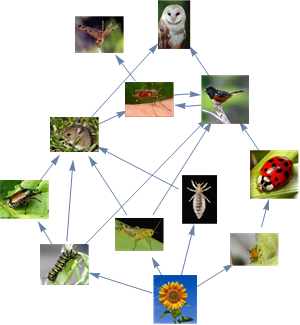
\includegraphics[width=0.38\textwidth]{foodweb.png}
\scriptsize
``SimpleFoodWeb" Mathematica sample network.
\caption{Using a network to represent relationships in a food web.}
\vspace{-15pt}
\label{fig:foodweb}
\end{wrapfigure}

Networks are first and foremost a way to model the relationships between objects, which we do by representing objects as vertices and their relationships as edges. For example, we might use a graph to represent the relationships in a food web, or between the individuals in a family tree.
%\footnote{The term \textit{network} is often used somewhat interchangeably with the term \textit{graph}. While they both refer to the same mathematical object, we attempt to follow the heuristic throughout of using the term \textit{graph} to refer to a purely mathematical object and \textit{network} to refer to a real-world system.} 

 In some cases, using this representation simply to visualize relationships is useful, but we generally would also like to computationally exploit it in order to gain further insight about the system we are modeling. As a first example, consider what questions we might ask about an infrastructure network such as a road network, phone lines, power grid, or the routers and fiber optic connections of the Internet itself. How do we efficiently get from here to there? How much traffic can flow through the network? What happens if an intersection is clogged, or a power plant fails? 

We can also ask questions about social networks representing relationships between people. Who is the most important? To what extent do the people you consider your friends consider themselves \textit{your} friend?  To what extent are your friends also friends with each other? To what extent do people form relationships with people who are like them? What do communities and strong friend groups look like mathematically?

One common question across all of mathematics is how similar objects are to each other. With networks, we can ask this question about individual vertices in a network, but we also frequently want to ask it about networks themselves. We may also want to define statistics that allow us to classify networks according to certain meaningful properties.

%For example, we might ask ``How similar are you to other students, based on your friendships at school?", but we can also ask ``Which proteins, protein interactions and groups of interactions are likely to have equivalent functions across species?" \cite{Sharan_2006}. 

For objects as combinatorially complex as networks, these kinds of comparisons present a difficult problem, the study of which has its roots in the 60s and 70s \cite{Conte_2004} and, as illustrated in Figure \ref{fig:year_distributions}, has gained significant attention in the past twenty years as interesting network data has become more readily available and the problem has become more computationally feasible.

\begin{figure}[t!]
\centering
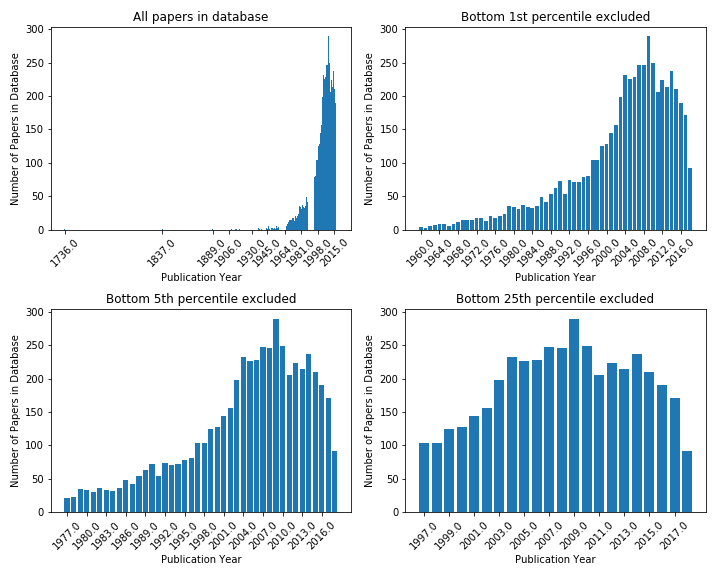
\includegraphics[width=0.9\textwidth]{year_distribution.png}
\caption{Distribution of papers published by year in our citation network of network similarity-related papers. Interestingly, year cutoffs for significant percentiles seem to roughly correspond to the spread of computers, personal computers, and the Internet, respectively.}
\label{fig:year_distributions}
\end{figure}

The goal of this project is to provide a broad outline of the comparative study of networks. Without the help of prior expertise in the field, however, it is difficult to determine which works are most relevant, and we therefore use the tools of network theory to study the network of citations between scientific papers on this topic. This allows us to use standard network analysis techniques to determine which papers are the most important or influential, and has the advantage of bringing transparency to the process. That is, we can quantitatively justify our assertions using standard centrality and community detection measures rather than relying on existing expertise in the field to give weight to our claims.

The rest of this work is structured as follows: In the remainder of this chapter, we introduce the necessary mathematical background to inform our analysis of our citation network dataset. In Chapters \ref{chapter:dataset_creation_and_analysis} and \ref{chapter:partitioning}, we introduce our citation network dataset. We analyze its basic structure, find two main fields of application within the study of network comparison, and choose a reading list from the high centrality vertices in our dataset. In Chapters \ref{chapter:pattern_recognition} and \ref{chapter:systems_biology}, we discuss our findings from this reading, and then conclude by discussing potential cross-applications between our two observed fields in Chapter 6.








\section{Background}

\begin{figure}[t]
\centering
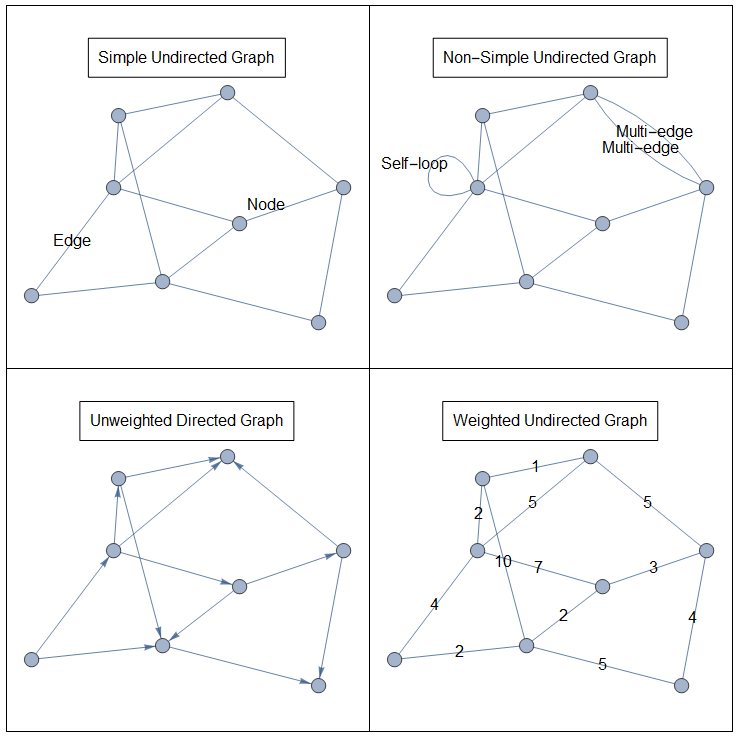
\includegraphics[width=0.9\textwidth]{basic_properties_demo.png}
\caption{Basic types of networks}
\label{fig:basic_properties_demo}
\end{figure}

We now introduce the definitions and notation required to give context to our analysis of the citation network. Our presentation follows Newman's \textit{Networks: An Introduction} \cite{newman2010} closely, with the remainder of definitions not otherwise cited sourced from \textit{Algorithms and Models for Network Data and Link Analysis} \cite{fouss2016}.

A \textbf{graph}\index{graph} $G(V,E)$ is formally defined as a finite nonempty set $V$ of \textbf{nodes}\index{nodes} or \textbf{vertices}\index{vertices} combined with a set $E\subset V\times V$ of \textbf{edges}\index{edges} representing relationships between pairs of vertices. Throughout this work, we denote the number of vertices in a graph by $n$ and the number of edges by $m$ where not otherwise specified.

In this work we will deal with \textbf{simple graphs}\index{simple graph}, which are those that do not have more than one edge between any pair of vertices (that is, a \textbf{multiedge}\index{multiedge}\footnote{A multigraph without edge loops is not simple, but if we represented the number of edges between pairs of vertices as edge weights instead of multiedges, that would be a simple graph.}) and do not have any edges from a vertex to itself (a \textbf{self-edge}\index{self-edge} or \textbf{self-loop}). 

We are also concerned with whether a graph is \textbf{directed}\index{directed graph} or \textbf{undirected}\index{undirected graph}. In an undirected graph, we have an edge \textit{between} two vertices, while in a directed graph we have edges \textit{from} one vertex to another vertex. Throughout this work, we will use the notation $v_i \leftrightarrow v_j$ for an undirected edge between vertices $v_i$ and $v_j$, and $v_i \rightarrow v_j$ for a directed edge. In either case, the edge $v_i\leftrightarrow v_j$ or $v_i\rightarrow v_j$ is \textbf{incident}\index{incident} to vertices $v_i$ and $v_j$, and vertices $v_i$ and $v_j$ are therefore considered \textbf{neighbors}\index{neighbor}.

A graph can also be \textbf{weighted}\index{weighted graph}, meaning each edge is assigned some real and generally positive value $w_{ij}$ representing the ``strength" of the connection between vertices $v_i$ and $v_j$. 

In an undirected graph, the \textbf{degree}\index{degree} of a vertex is the sum of the weights of the incident edges. In a directed graph, the \textbf{indegree}\index{indegree} and \textbf{outdegree}\index{outdegree} are the total weight of a vertex's incoming and outgoing edges, respectively. If the graph is unweighted, this is simply the number of adjacent, incoming, or outgoing edges, as the weight of each edge is one.

When studying real-world networks, we also make a distinction between \textbf{deterministic}\index{deterministic} and \textbf{random}\index{random} networks. This distinction is roughly the same as that between a variable and a random variable. The vertices and edges in a deterministic network are ``fixed", while in a random network they need to be inferred from data using statistical inference methods. For example, our citation network is deterministic, but a network of protein interactions for a given species is not, as it must be inferred from experimental data on a limited number of members of that species.

\subsection{Computational network properties}
Whether a network is directed or weighted or simple will inform our approach to its analysis, but these properties are generally included as metadata rather than computationally determined. The remainder of the properties we consider in network analysis are determined computationally, and their calculation involves varying degrees of algorithmic complexity.

\subsubsection{Connectivity}

\begin{wrapfigure}{L}{0.3\textwidth}
\centering
\vspace{-5pt}
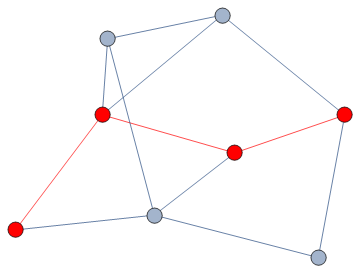
\includegraphics[width=0.28\textwidth]{path_demo.png}
\caption{A path of length three on a small network.}
\vspace{-10pt}
\label{fig:path_demo}
\end{wrapfigure}

One fairly intuitive but particularly relevant network property is the question of whether a network is \textbf{connected}\index{connected graph}, as illustrated in Figure \ref{fig:connectivity_demo}; that is, there is a path between any pair of vertices, where a  \textbf{path}\index{path} is defined to be a sequence of vertices $\{v_1, v_2, \dots, v_n\}$ such that consecutive vertices are connected by an edge. In the case of a directed graph, the edges in a path must run from $v_1$ to $v_2$ and $v_2$ to $v_3$ and so on; they cannot go backwards. The \textbf{length}\index{path length} of a path is the number of edges connecting the vertices in the sequence. In the case of a directed graph, we make a distinction between \textit{weak} and \textit{strong} connectivity. A \textbf{weakly connected graph}\index{weakly connected graph} is one which is connected when each directed edge is considered as undirected, while a \textbf{strongly connected graph}\index{strongly connected graph} requires a path from every vertex to every other vertex that respects edge directions. 

\begin{figure}[t]
\centering
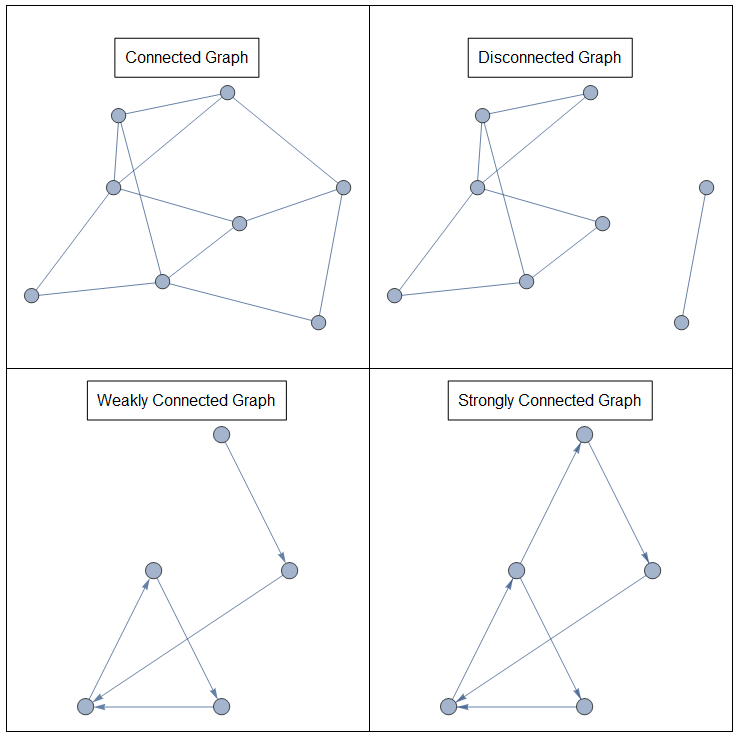
\includegraphics[width=0.9\textwidth]{connectivity_demo.png}
\caption{Simple examples of different types of network connectivity.}
\label{fig:connectivity_demo}
\end{figure}

If an undirected network is not connected or a directed network is not weakly or strongly connected, the network has multiple \textbf{connected components}\index{connected component} or \textbf{weakly connected components}\index{weakly connected component}. Each component is a subset of vertices such that there is a path between every pair of member vertices and no paths between any member and a nonmember. For example, the disconnected graph in Figure \ref{fig:connectivity_demo} has two components. The weakly connected components of a directed graph are the components in the corresponding undirected network.

In a typical real-world network, there is usually a single large component or weakly connected component which contains most of the vertices, with the rest of the vertices contained in many small components. We call this large component the \textbf{giant component}\index{giant component}, and its relative size tells us how close a network is to being connected.

\subsubsection{Assortativity}

\begin{figure}[t!]
\centering
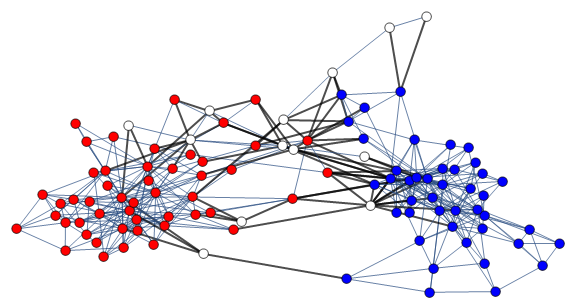
\includegraphics[width=0.6\textwidth]{assortativity_demo.png}

\scriptsize
``USPoliticsBooks" Mathematica sample network.
\caption{A strongly assortative network of U.S. politics books. Books categorized as liberal, conservative, or neutral are colored blue, red, and white, respectively, and edges that run between different categories are bolded.}
\label{fig:assortativity_demo}
\end{figure}

We can also consider whether a network is \textbf{assortative}\index{assortative}. That is, if the vertices in the network have some discrete-valued property, we ask whether the edges in the network are more likely to run between vertices of the same type. If all of the edges run between vertices of the same type, the assortativity of the network is 1; if all edges run between edges of different types, the assortativity is $-1$.

For example, the network of U.S. politics books in Figure \ref{fig:assortativity_demo} is strongly assortative with an assortativity value of $0.72$. Most of the connections are between books with the same political classification, which we can visually confirm by coloring the vertices accordingly and highlighting the few edges of the graph that run between books with different classifications.

\subsubsection{Acyclic networks}

We also consider whether a directed network is \textbf{acyclic}\index{directed acyclic network}, meaning that it contains no \textbf{cycles}\index{cycle} or nontrivial paths from any vertex to itself. See Figure \ref{fig:acyclic_demo}.

One example of a directed acyclic network is a \textbf{citation network}\index{citation network}. In a citation network, we include an edge from a paper to each reference it cites. Any cycle in this network would require edges both from a newer paper to an older paper and from an older paper to a newer paper. If we only cite papers which have already been written, which is the case for the papers in our dataset and generally true for academia as a whole, we cannot have any cycles. 

\begin{figure}[t!]
\centering
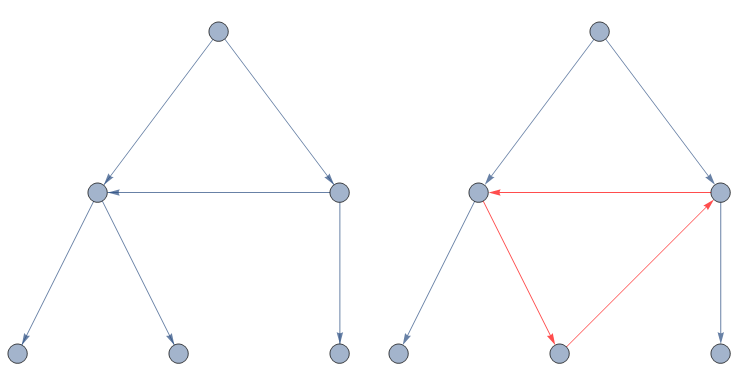
\includegraphics[width=0.58\textwidth]{acyclic_demo.png}
\caption{An acyclic directed network (left) vs. one which contains a cycle (right).}
\label{fig:acyclic_demo}
\end{figure}







%%%%%%%%%%%%%%%%%%%%%%%%%%%%%%%% CHAPTER 2 %%%%%%%%%%%%%%%%%%%%%%%%%%%%%%%%%%%%%%%









\chapter{Creating the citation network}\label{chapter:dataset_creation_and_analysis}

\section{Approach}

Citation network creation is not a trivial task. Although some journals and databases provide a citation network of the references in their own domain, the field we are considering is highly interdisciplinary; investigating only the citations within a single database or journal would discard large sections of the desired network. As a result, and since intellectual property restrictions preclude directly scraping an entire citation network, we constructed the dataset manually from the reference lists of relevant papers.

Relevant papers were found by searching Google Scholar for ``graph" or ``network" +  ``alignment", ``comparison", ``similarity", ``isomorphism", or ``matching"\footnote{Future work may want to include ``graph kernel(s)" in this list.}. Topic-relevant papers were initially collected from the first five pages of results for each of these ten search terms on May 4th, 2018, after which new papers published through June 25th, 2018 were collected from a Google Scholar email alert for those same ten search terms. For each of these papers, we stored the plaintext reference list in a standardized format which could be easily split into the individual freeform citations. Any paper for which we have a reference list is referred to as a ``parent" record, and the references are referred to as the ``child" records. In total, we collected 7,790 child references from 221 parent papers.

In order to create the network, we needed to parse the freeform citations for each reference list to obtain metadata and be able to recognize records as being cited multiple times. This is a difficult problem, as the records in the database span several hundred years and represent a wide variety of citation styles and languages, while also presenting significant optical character recognition and Unicode-related challenges. Instead of attempting to parse a citation into component parts, we used the REST API \cite{crossrefAPI} to search for each record in the CrossRef database, which already has metadata parsed for any record it includes. We marked results as duplicate if their metadata matched and both were known to be correct, or if both their metadata and freeform citation match exactly. 

We considered the results given by the REST API to be correct if the title of the record could be found in the original freeform citation and unverified otherwise. We were able to automatically verify results for about 75\% of the parent records and about half of their children. We were conservative about marking records as duplicate, which meant that having so many unverified records would dramatically misrepresent the structure of the network. We therefore went through the unverified records by hand.

For unverified parents, we manually found title, year, author, DOI, and URL information as well as reference and citation counts. For unverified children, we first went through and marked any correct but unverified results; about half of the unverified child results were correct but unable to be automatically verified due to punctuation discrepancies, misspellings, unicode issues, or citation styles that do not include the title. Next, we counted results as correct but marked them as ``half-right" if the REST API returned a review, purchase listing, or similar for the correct record. For the remaining incorrect references, we manually added the author, title, and year from the citation. Finally, we deleted any records which did not refer to a written work of some kind, i.e, those citing a website, web service, database, software package/library, programming language, or ``personal communication".

We then wrote the entire citation network to a GML file which could be loaded in Mathematica. By default, the code used to generate the GML file includes the title, year, and reference and citation counts for each record as vertex properties. Including further metadata is not difficult, but additional string-valued properties dramatically slow Mathematica's ability to load such a large network\footnote{The network contains 5,793 vertices and 7,491 edges and takes two minutes to load on a 2.6GHz 6th-gen quad core Intel Core i7 CPU with 16GB of RAM running Windows 10 using Mathematica 11.2.}, and a network as large as ours could not be loaded at all. We therefore did not include any more string-valued properties than strictly necessary.

The dataset itself and the code and source files used to generate it can be found at \url{https://github.com/marissa-graham/network-similarity}, along with documentation and instructions for using it to generate a similar dataset for any collection of properly-formatted reference list files.

\begin{figure}[p]
\centering
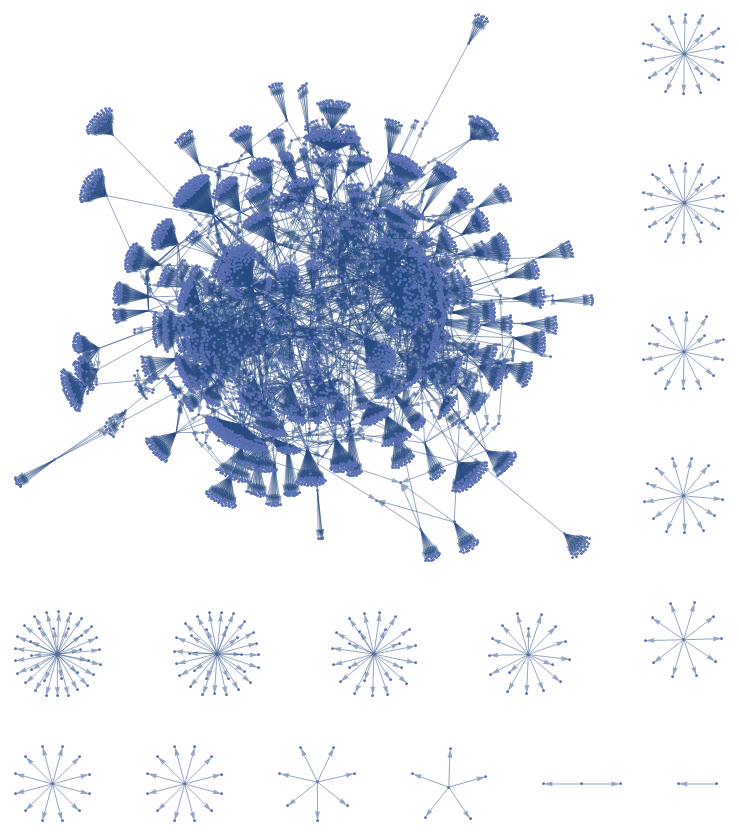
\includegraphics[width=0.9\textwidth]{full_citation_network.png}
\caption{The full citation network of the dataset used for the project.}
\label{fig:full_database}
\end{figure}








\section{Basic statistics}

\subsubsection{Construction-related issues}

Our full citation network contains a total of 7,491 references between 5,793 papers. This results in a fairly low mean degree (i.e., average number of references per paper), which is an inherent limitation in the construction of almost any citation network. We can include all the references for a small group of papers, but including all the references for \textit{their} references and so on is an exponentially more expensive task, and we therefore generally only include children for a small fraction of the total vertices. 

Since the edges in our network are hand-constructed using individual reference lists, it contains an abnormally small fraction of vertices with children. A typical citation network, such as the SciMet and Zewail datasets included in Table \ref{tab:network_table} and shown in Figures \ref{fig:sciMet} and \ref{fig:zewail} respectively, is constructed by scraping a single database. They contain a larger fraction of children whose references are included than our citation network, but any references not in that particular database are missed; their mean degrees are therefore still quite low.

\begin{table}[t!]
\centering
\setlength\extrarowheight{2pt}
\begin{tabular}{|p{0.31\linewidth}|R{0.07\linewidth}|R{0.07\linewidth}|R{0.085\linewidth}|R{0.08\linewidth}|R{0.07\linewidth}|R{0.07\linewidth}|}
\hline
 & $G$ & $G_p$ & SciMet & Zewail & $R$ & $R_d$ \\ \hline\hline% & $R_{d,p}$ \\ \hline\hline
Vertices & 5793 & 1062 & 1092 & 3145 & 5793 & 5793 \\ \hline % & 1077 \\ \hline %
Edges & 7491 & 2775 & 1308 & 3743 & 7491 & 7491\\ \hline % & 2775 \\ \hline
Mean degree & 1.29 & 2.61 & 1.20 & 1.19 & 1.29 & 1.29 \\ \hline %& 2.58 \\ \hline
Fraction with children & 0.038 & 0.193 & 0.523 & 0.599 & 0.733 & 0.038 \\ \hline %& 0.202\\ \hline
Diameter & 10 & 9 & 14 & 22 & 21 & 9\\ \hline % & 7 \\ \hline
Connected components & 16 & 1 & 114 & 281 & 504 & 3 \\ \hline %& 3\\ \hline
Fraction in giant component & 0.960 & 1.000 & 0.784 & 0.797 & 0.900 & 0.999 \\ \hline %& 1.000 \\ \hline
%Assortativity by indegree & 0.113 & 0.016 & 0.055 & 0.158 & 0.007 & -0.008\\ \hline % & -0.007 \\ \hline
%Assortativity by outdegree & -0.014 & -0.014 & -0.025 & 0.056 & -0.018 & -0.007 \\ \hline %& -0.013 \\ \hline
\end{tabular}
\caption{Comparing statistics for our dataset to other networks.}

\label{tab:network_table}
\end{table}

\subsubsection{The pruned network $G_p$}

\begin{figure}[h]
\centering
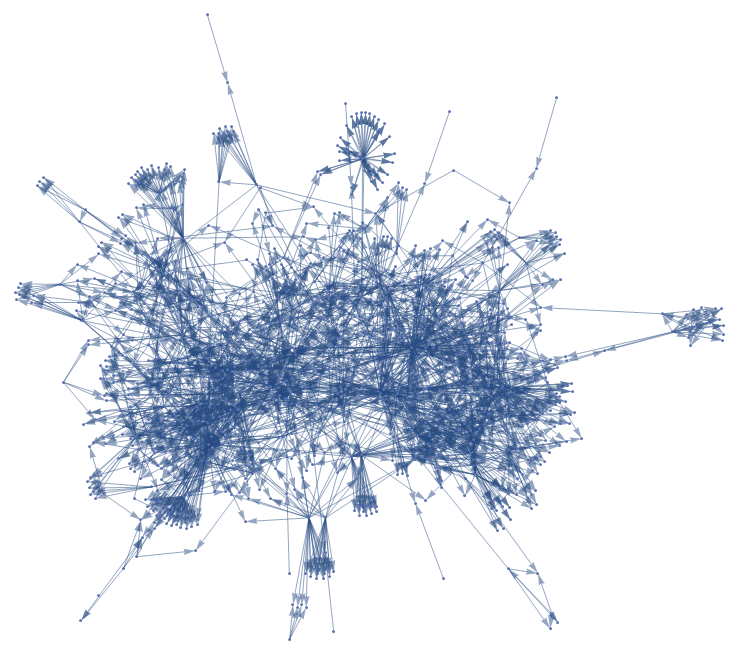
\includegraphics[width=0.9\textwidth]{subnetwork.png}
\caption{The pruned citation network.}
\label{fig:pruned_network}
\end{figure}

We also consider the \textit{pruned network}, shown in Figure \ref{fig:pruned_network}, which we define to be the giant component of the subnetwork of vertices with positive outdegree or indegree greater than one. That is, we discard any papers which are not part of the giant component and child papers which are not cited by multiple parents. We do so because the main purpose of our dataset is to determine which papers are important in the field of network similarity, but the vast majority of references in the database are only cited by one paper and frequently have very little relevance to network similarity itself. Overall, this restriction shrinks the number of vertices by a factor of almost six, correspondingly raises the fraction of vertices with children, and approximately doubles the mean degree (i.e, the number of edges divided by the number of vertices).

\subsubsection{Comparison to other networks}
In Table \ref{tab:network_table}, we calculate the mean degree, fraction of vertices with children, diameter, number of connected components, and fraction of vertices in the giant component for six different networks: our full network $G$, its pruned version $G_p$, two datasets from the Garfield citation network collection, a uniformly generated directed random graph $R$, and a random graph $R_d$ with the same degree sequences as $G$. The random network $R$ is generated from a uniform distribution. The other, $R_d$, is constructed\footnote{We note that the construction method of $R_d$ does not exclude multiedges. This does not pose a problem here, but allowing multiedges would cause issues with our analysis of graphlet degree distributions of protein-protein interaction networks as shown in Figure \ref{fig:GDD_demo}. In that case, we exclude multiedges in our construction of the random networks matching the degree distribution.} to match the degree sequence of $G$.

\subsubsection{Connectivity}

Our full network displays a high level of connectivity. It has 96\% of its vertices contained in the giant component and only 16 connected\footnote{For all our citation network variations, we consider the weakly connected components.} components total, compared to 90\% containment in the giant component and 504 connected components for a randomly generated network of the same size. The diameter is also low compared to a random network and to our choices of real-world network. Since our network consists of papers collected on a specific topic (which have an outside reason to cite the same papers), this high level of connectivity is not surprising. 

The construction method of our network also explains its high connectivity compared to our real-world datasets, which only have about 80\% of their vertices in their giant components. If the generation of the citation network is limited to a single database, as the SciMet and Zewail datasets are, cocitation connections in other databases will be lost. This makes it more difficult for the giant component to fill the network and results in longer paths between connected vertices.

The only dataset tested with better connectivity than ours is the random network $R_d$, which has almost complete containment--$99.9\%$--in the giant component. This is not surprising. Approximately speaking, in order for a parent vertex to be disconnected from the giant component, its children must all have exactly one parent and no children.  In a real-world network, this can occur naturally, because a paper's references are not randomly selected. A single work which is relatively disconnected from the rest of the community can generate a significant number of references which are not in the giant component. By contrast, since about 82\% of the vertices in $G$ have exactly one parent and no children, the probability of a parent vertex with outdegree $n$ being disconnected from the giant component is $(0.82)^n$, or $(0.82)^{26.2} \approx 0.5\%$ for the mean outdegree of the parents in our network. This probability shrinks further as the number of disconnected parent vertices grows, as fewer single-parent vertices become available compared to the rest.








\section{Centrality}\label{section:centrality}

Our main goal in creating this citation network was to determine which papers are most important or \textbf{central}\index{centrality}. The question of which vertices are the most central to a network is widely researched in network theory, and there correspondingly exists a wide variety of centrality measures used to quantify different ideas about importance. For this project, we chose five centrality measures that we expect to coincide with an intuitive definition of which papers in the network are the most relevant. Our definitions of these come from \cite{newman2010}.

\subsubsection{Indegree} This measures the number of times each paper was cited by the parent papers in our network. Since the parent papers approximately represent everything determined to be most relevant by Google Scholar in a search for network comparison-related search terms\footnote{This is somewhat skewed by our inclusion of newly published papers collected from an email alert after the initial search, which may not be the most relevant overall.}, the top values for indegree should give us a rough idea of which papers are formative for the field and therefore more frequently cited by the parent papers.

\subsubsection{Outdegree}\index{degree centrality} Since the pruned network consists of the parent papers as well as the papers that appear in more than one parent's reference list, this measures the number of a parent's references which have been cited by other parents in the network. The papers with highest outdegree are therefore those which survey the most well-known topics in the field.

\subsubsection{Betweenness}\index{betweenness centrality} Betweenness centrality measures the extent to which a vertex lies on paths between other vertices. Intuitively, this should correspond to papers which make uncommon connections between other works: those that are applicable to a wide variety of fields and applications, and those which build on disparate ideas in an original way. Unsurprisingly, we see some overlap between the papers with the highest outdegree and those with the highest betweenness.

\subsubsection{Closeness} 

\begin{figure}[b!]
\centering
%\captionsetup{width=.9\linewidth}
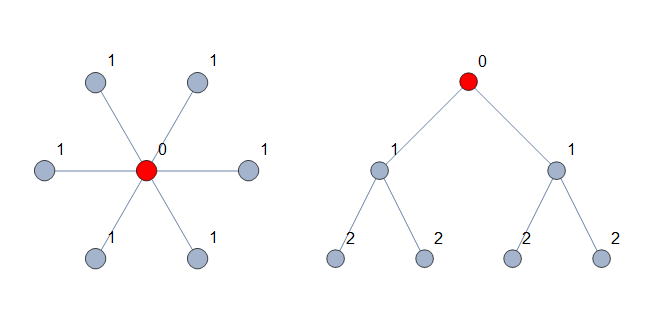
\includegraphics[width=0.65\textwidth]{closeness_demo.png}
\vspace{-10pt}
\caption{Geodesic distances from the highlighted vertex for two different graphs.}
\label{fig:closeness_demo}
\end{figure}

Recall that a path between two vertices is a sequence of vertices such that consecutive vertices are connected by an edge. A \textbf{geodesic path}\index{geodesic path} is the shortest possible path between any two vertices, and its length is the \textbf{geodesic distance}\index{geodesic distance}. We define \textbf{closeness}\index{closeness centrality} to be the inverse of the average geodesic distance between a vertex and all other vertices in the network. Closeness centrality therefore takes on the highest values for a vertex which has a short average distance from all other vertices. For example, in Figure \ref{fig:closeness_demo} the highlighted vertex on the left has closeness centrality 1, since it has a distance of 1 from all other vertices. On the right, the average geodesic distance from the highlighted vertex to the other six is $\frac{1}{6}(1+1+2+2+2+2)=\frac{5}{3}$, so the closeness centrality is 0.6.

A paper in our citation network has high closeness centrality if it only takes a few steps through a paper's reference list or citations to another paper's reference list or citations to get to every other paper in the network. 

\subsubsection{HITS}
For a directed network such as the citation networks used here, we may want to separately consider the notion that a vertex is important if it points to other important vertices, and the notion that a vertex is important if it is pointed to by other important vertices. This is the goal of the HITS (hyperlink-induced topic search) algorithm. It defines two different types of centrality for each vertex. The \textbf{authority centrality}\index{authority centrality} of a vertex measures whether it is being pointed to by vertices with high \textbf{hub centrality}\index{hub centrality}, which in turn measures whether those vertices point to vertices with high authority centrality. By defining the hub and authority centralities of a vertex to be proportional to the sum of the authority and hub centralities, respectively, of its neighbors, this definition reduces to a pair of eigenvalue equations which can be easily solved numerically. 

That is, if $x_i$ is the authority centrality of the $i$-th vertex in a network, $y_i$ is the hub centrality of the $j$-th vertex, $A_{ij}$ is the weight of the edge from $j$ to $i$ if it exists, and 0 otherwise, and $\alpha, \beta$ are proportionality constants, we have
\[x_i = \alpha \sum_j A_{ij}y_j\text{ and } y_i = \beta \sum_j A_{ji}x_j.\]

\subsection{High centrality vertices}\label{section:high_centrality_vertices}

We can see that the pruned network shown in Figure \ref{fig:pruned_network} contains two clusters of more tightly connected vertices\footnote{We discuss the motivation behind and significance of this partition in detail in Chapter \ref{chapter:partitioning}.}; this is even more clear in Figure \ref{fig:partitioned_network}. We would like to collect the important papers for both the network as a whole and for these two communities, so we partition the dataset in half using a modularity maximizing partition; that is, we choose two groups of vertices such that the fraction of edges running between vertices in different groups is minimized.

For both the pruned network and the two halves of our partition, we collect the top ten papers according to these five different centrality measures and summarize the results in the following tables. Since the numerical values for indegree and outdegree have intuitive meaning, we report the value itself. However, the values for betweenness, closeness, and the two HITS centralities are unintuitive, context-free real numbers, so we report the rank of each paper with respect to each of these measures rather than the actual value. We also calculate betweenness and closeness for the undirected version of the network in order to allow those rankings to be based on citing relationships in either direction.

The papers in each table are sorted from maximum to minimum with respect to \[ f(p) = \frac{k^{in}_p}{k^{in}_{max}} + \frac{k^{out}_p}{ k^{out}_{max}} + \sum_{i=1}^4 \frac{1}{r_i(p)}, \] where $k^{in}_p$ and $k^{out}_p$ are the indegree and outdegree of a paper $p$, the maximums of which are taken with respect to the pruned network or partition half in question, and $r_i(p)$ is the rank of a paper $p$ according to the $i$-th of our four centrality metrics, which is defined to be infinity if a paper is not in the top ten for that metric. In all three tables, a $^*$ indicates that a paper's indegree or outdegree is ranked top ten within the relevant network.
 
\begin{table}[H]
\centering
\vspace{-.5cm}
{\setlength\extrarowheight{2pt}\setlength{\tabcolsep}{3pt}\setstretch{1}\fontsize{10}{13}\selectfont
\begin{tabular}{|L{0.75\linewidth}|c|c|c|c|c|c|}
\hline
& \rotatebox[origin=c]{90}{Indegree} &  \rotatebox[origin=c]{90}{Outdegree} & \rotatebox[origin=c]{90}{Betweenness} &  \rotatebox[origin=c]{90}{Closeness} &  \rotatebox[origin=c]{90}{HITS Auth.} & \rotatebox[origin=c]{90}{HITS Hub} \\ 
\hline\hline
$^\Diamond$Thirty years of graph matching in pattern recognition  \cite{Conte_2004} & 20* & 109* & 1 & 2 &  & 1 \\ \hline
$\dagger$Fifty years of graph matching, network alignment and network comparison  \cite{Emmert_Streib_2016} & 6 & 71* & 2 & 1 &  & 3 \\ \hline
$\dagger$Networks for systems biology: Conceptual connection of data and function  \cite{Emmert_Streib_2011} & 2 & 102* & 3 & 3 &  & 2 \\ \hline
$^\Diamond$An algorithm for subgraph isomorphism  \cite{Ullmann_1976} & 20* & 4 & 7 & 4 & 1 &  \\ \hline
$\dagger$Modeling cellular machinery through biological network comparison  \cite{Sharan_2006} & 9 & 41* & 8 &  &  &  \\ \hline
$^\Diamond$Computers and intractability: A guide to the theory of NP-completeness  \cite{Hartmanis_1982} & 16* & 0 & 4 & 5 &  &  \\ \hline
$^\Diamond$The graph matching problem  \cite{Livi_2012} & 2 & 55* & 5 & 6 &  & 7 \\ \hline
$\dagger$A new graph-based method for pairwise global network alignment  \cite{Klau_2009} & 9 & 13 &  & 8 &  &  \\ \hline
$\dagger$On graph kernels: Hardness results and efficient alternatives  \cite{Gartner_2003} & 11 & 10 & 6 &  &  &  \\ \hline
$^\Diamond$Error correcting graph matching: On the influence of the underlying cost function  \cite{Bunke_1999} & 10 & 16 &  & 7 & 7 & 8 \\ \hline
$^\Diamond$A graduated assignment algorithm for graph matching  \cite{Gold_1996} & 18* & 0 &  &  & 5 &  \\ \hline
$^\Diamond$The Hungarian method for the assignment problem  \cite{Kuhn_1955} & 17* & 0 &  &  &  &  \\ \hline
$^\Diamond$An eigendecomposition approach to weighted graph matching problems  \cite{Umeyama_1988} & 15* & 5 &  &  & 6 &  \\ \hline
$^\Diamond$Recent developments in graph matching  \cite{Bunke_2000} & 1 & 51* &  &  &  & 4 \\ \hline
$\dagger$MAGNA: Maximizing accuracy in global network alignment  \cite{Saraph_2014} & 5 & 35* &  &  &  &  \\ \hline
$^\Diamond$A distance measure between attributed relational graphs for pattern recognition  \cite{Sanfeliu_1983} & 14* & 0 &  &  & 3 &  \\ \hline
$\dagger$Pairwise global alignment of protein interaction networks by matching neighborhood topology  \cite{Singh_2007} & 13* & 0 &  &  &  &  \\ \hline
$\dagger$Topological network alignment uncovers biological function and phylogeny  \cite{Bunke_1998} & 12* & 0 &  &  &  &  \\ \hline
A graph distance metric based on the maximal common subgraph  \cite{Kuchaiev_2010} & 10 & 0 &  & 10 & 4 &  \\ \hline
$^\Diamond$Efficient graph matching algorithms  \cite{Messmer_1995} & 0 & 43* &  &  &  & 5 \\ \hline
Local graph alignment and motif search in biological networks  \cite{Berg_2004} & 8 & 10 & 10 &  &  &  \\ \hline
$\dagger$Global alignment of multiple protein interaction networks with application to functional orthology detection  \cite{Singh_2008} & 11* & 0 &  &  &  &  \\ \hline
On a relation between graph edit distance and maximum common subgraph  \cite{Bunke_1997} & 11 & 0 &  &  & 2 &  \\ \hline
$^\Diamond$Graph matching applications in pattern recognition and image processing  \cite{Conte_2003} & 0 & 40* &  &  &  & 6 \\ \hline
$^\Diamond$Fast and scalable approximate spectral matching for higher order graph matching  \cite{Park_2014} & 0 & 41* & 9 &  &  &  \\ \hline
$^\Diamond$Structural matching in computer vision using probabilistic relaxation  \cite{Christmas_1995} & 9 & 0 &  &  & 10 &  \\ \hline
$^\Diamond$A new algorithm for subgraph optimal isomorphism  \cite{El_Sonbaty_1998} & 2 & 21 &  &  &  & 9 \\ \hline
BIG-ALIGN: Fast bipartite graph alignment  \cite{Koutra_2013} & 2 & 21 &  & 9 &  &  \\ \hline
$^\Diamond$A graph distance measure for image analysis  \cite{Eshera_1984} & 8 & 0 &  &  & 8 &  \\ \hline
A new algorithm for error-tolerant subgraph isomorphism detection  \cite{Messmer_1998} & 8 & 0 &  &  & 9 &  \\ \hline
$^\Diamond$A (sub)graph isomorphism algorithm for matching large graphs  \cite{Cordella_2004} & 3 & 16 &  &  &  & 10 \\ \hline
\end{tabular}

\vspace{-.01cm}
$\dagger$Also top for Group 1 (biology dominated); $^\Diamond$Also top for Group 2 (computer science dominated)
}
\vspace{-.22cm}
\caption{Highest centrality papers for the entire pruned network.}
\label{tab:toppapers_all}
\end{table}

\begin{table}[H]
\centering
\vspace{-.5cm}
{\setlength\extrarowheight{2pt}\setlength{\tabcolsep}{3pt}\setstretch{1}\fontsize{10}{13}\selectfont
\begin{tabular}{|L{0.75\linewidth}|c|c|c|c|c|c|}
\hline
& \rotatebox[origin=c]{90}{Indegree} &  \rotatebox[origin=c]{90}{Outdegree} & \rotatebox[origin=c]{90}{Betweenness} &  \rotatebox[origin=c]{90}{Closeness} &  \rotatebox[origin=c]{90}{HITS Auth.} & \rotatebox[origin=c]{90}{HITS Hub} \\ 
\hline\hline
$^\Diamond$Networks for systems biology: Conceptual connection of data and function  \cite{Emmert_Streib_2011} & 2 & 90* & 1 & 2 &  & 1 \\ \hline
$^\Diamond$Fifty years of graph matching, network alignment and network comparison  \cite{Emmert_Streib_2016} & 4 & 56* & 2 & 1 &  & 2 \\ \hline
$^\Diamond$Modeling cellular machinery through biological network comparison  \cite{Sharan_2006} & 9 & 40* & 4 & 3 & 10 & 9 \\ \hline
$^\Diamond$MAGNA: Maximizing accuracy in global network alignment  \cite{Saraph_2014} & 5 & 35* & 7 & 6 &  & 3 \\ \hline
$^\Diamond$On graph kernels: Hardness results and efficient alternatives  \cite{Gartner_2003} & 10* & 9 & 3 & 8 &  &  \\ \hline
Biological network comparison using graphlet degree distribution  \cite{Przulj_2007} & 11* & 0 &  & 7 & 4 & 7 \\ \hline
$^\Diamond$A new graph-based method for pairwise global network alignment  \cite{Klau_2009} & 8 & 12 & 9 & 4 & 6 &  \\ \hline
Network motifs: Simple building blocks of complex networks  \cite{Milo_2002} & 11* & 0 &  & 9 & 8 &  \\ \hline
$^\Diamond$Pairwise global alignment of protein interaction networks by matching neighborhood topology  \cite{Singh_2007} & 12* & 0 &  &  & 3 &  \\ \hline
$^\Diamond$Topological network alignment uncovers biological function and phylogeny  \cite{Kuchaiev_2010} & 12* & 0 &  &  & 2 &  \\ \hline
NETAL: A new graph-based method for global alignment of protein-protein interaction networks  \cite{Neyshabur_2013} & 6 & 26* &  &  &  & 5 \\ \hline
Collective dynamics of ``small-world" networks  \cite{Watts_1998} & 10* & 0 &  & 10 & 5 &  \\ \hline
Global network alignment using multiscale spectral signatures  \cite{Patro_2012} & 11* & 0 &  &  & 9 &  \\ \hline
$^\Diamond$Global alignment of multiple protein interaction networks with application to functional orthology detection  \cite{Singh_2008} & 10* & 0 &  &  &  &  \\ \hline
Conserved patterns of protein interaction in multiple species  \cite{Sharan_2005} & 10* & 0 &  &  & 7 &  \\ \hline
Pairwise alignment of protein interaction networks  \cite{Koyuturk_2006} & 10* & 0 &  &  & 1 &  \\ \hline
Alignment-free protein interaction network comparison  \cite{Ali_2014} & 2 & 22 & 6 & 5 &  &  \\ \hline
Graphlet-based measures are suitable for biological network comparison  \cite{Hayes_2013} & 1 & 30* &  &  &  & 8 \\ \hline
Survey on the graph alignment problem and a benchmark of suitable algorithms  \cite{Dopmann_2013} & 0 & 26 &  &  &  & 4 \\ \hline
Predicting graph categories from structural properties  \cite{Canning_2018} & 0 & 30* & 5 &  &  &  \\ \hline
Fast parallel algorithms for graph similarity and matching  \cite{Kollias_2014} & 1 & 23 &  &  &  & 6 \\ \hline
Complex network measures of brain connectivity: Uses and interpretations  \cite{Rubinov_2010} & 0 & 28* & 8 &  &  &  \\ \hline
Graph-based methods for analysing networks in cell biology  \cite{Aittokallio_2006} & 0 & 30* &  &  &  & 10 \\ \hline
Demadroid: Object reference graph-based malware detection in android  \cite{Wang_2018} & 0 & 25 & 10 &  &  &  \\ \hline
Early estimation model for 3D-discrete Indian sign language recognition using graph matching  \cite{Kumar_2018a} & 0 & 29* &  &  &  &  \\ \hline
Indian sign language recognition using graph matching on 3D motion captured signs  \cite{Kumar_2018b} & 0 & 29* &  &  &  &  \\ \hline
\end{tabular}

\vspace{-.01cm}
$^\Diamond$Also a top-centrality paper for the entire network}
\vspace{-.22cm}
\centering
\caption{Highest centrality papers for the biology-dominated half of the pruned network.}
\label{tab:toppapers_bio}
\end{table}

\begin{table}[H]
\centering
\vspace{-.5cm}
{\setlength\extrarowheight{2pt}\setlength{\tabcolsep}{3pt}\setstretch{1}\fontsize{10}{13}\selectfont
\begin{tabular}{|L{0.75\linewidth}|c|c|c|c|c|c|}
\hline
& \rotatebox[origin=c]{90}{Indegree} &  \rotatebox[origin=c]{90}{Outdegree} & \rotatebox[origin=c]{90}{Betweenness} &  \rotatebox[origin=c]{90}{Closeness} &  \rotatebox[origin=c]{90}{HITS Auth.} & \rotatebox[origin=c]{90}{HITS Hub} \\ 
\hline\hline
$^\Diamond$Thirty years of graph matching in pattern recognition  \cite{Conte_2004} & 17* & 107* & 1 & 1 &  & 1 \\ \hline
$^\Diamond$An algorithm for subgraph isomorphism  \cite{Ullmann_1976} & 15* & 2 & 10 & 5 & 2 &  \\ \hline
$^\Diamond$A graduated assignment algorithm for graph matching  \cite{Gold_1996} & 18* & 0 & 7 & 4 & 3 &  \\ \hline
$^\Diamond$An eigendecomposition approach to weighted graph matching problems  \cite{Umeyama_1988} & 15* & 5 &  & 2 & 4 &  \\ \hline
$^\Diamond$The graph matching problem  \cite{Livi_2012} & 2 & 36* & 3 & 3 &  & 8 \\ \hline
$^\Diamond$A distance measure between attributed relational graphs for pattern recognition  \cite{Sanfeliu_1983} & 13* & 0 &  & 7 & 1 &  \\ \hline
$^\Diamond$Recent developments in graph matching  \cite{Bunke_2000} & 0 & 50* & 8 &  &  & 2 \\ \hline
$^\Diamond$Error correcting graph matching: On the influence of the underlying cost function  \cite{Bunke_1999} & 9* & 16 &  & 8 &  & 6 \\ \hline
$^\Diamond$Fast and scalable approximate spectral matching for higher order graph matching  \cite{Park_2014} & 0 & 41* & 2 &  &  &  \\ \hline
$^\Diamond$Efficient graph matching algorithms  \cite{Messmer_1995} & 0 & 42* & 5 &  &  & 4 \\ \hline
$^\Diamond$Computers and intractability: A guide to the theory of NP-completeness  \cite{Hartmanis_1982} & 11* & 0 & 6 &  &  &  \\ \hline
$^\Diamond$The Hungarian method for the assignment problem  \cite{Kuhn_1955} & 14* & 0 &  &  &  &  \\ \hline
$^\Diamond$Graph matching applications in pattern recognition and image processing  \cite{Conte_2003} & 0 & 40* &  &  &  & 3 \\ \hline
Efficient graph similarity search over large graph databases  \cite{Zheng_2015} & 0 & 28* & 4 & 6 &  &  \\ \hline
A linear programming approach for the weighted graph matching problem  \cite{Almohamad_1993} & 8 & 8 &  & 9 & 9 &  \\ \hline
$^\Diamond$Structural matching in computer vision using probabilistic relaxation  \cite{Christmas_1995} & 9* & 0 &  &  & 5 &  \\ \hline
$^\Diamond$A graph distance measure for image analysis  \cite{Eshera_1984} & 8 & 0 &  &  & 6 &  \\ \hline
Inexact graph matching for structural pattern recognition  \cite{Bunke_1983} & 10* & 0 &  &  &  &  \\ \hline
$^\Diamond$A new algorithm for subgraph optimal isomorphism  \cite{El_Sonbaty_1998} & 2 & 21 &  &  &  & 5 \\ \hline
Approximate graph edit distance computation by means of bipartite graph matching  \cite{Riesen_2009} & 9 & 0 &  &  &  &  \\ \hline
Linear time algorithm for isomorphism of planar graphs  \cite{Hopcroft_1974} & 9 & 0 &  &  &  &  \\ \hline
Structural descriptions and inexact matching  \cite{Shapiro_1981} & 9 & 0 &  &  & 7 &  \\ \hline
$^\Diamond$A (sub)graph isomorphism algorithm for matching large graphs  \cite{Cordella_2004} & 3 & 16 &  &  &  & 7 \\ \hline
A probabilistic approach to spectral graph matching  \cite{Egozi_2013} & 0 & 25* & 9 & 10 &  &  \\ \hline
Hierarchical attributed graph representation and recognition of handwritten chinese characters  \cite{Lu_1991} & 6 & 0 &  &  & 8 &  \\ \hline
Exact and approximate graph matching using random walks  \cite{Gori_2005} & 1 & 14 &  &  &  & 9 \\ \hline
A shape analysis model with applications to a character recognition system  \cite{Rocha_1994} & 5 & 0 &  &  & 10 &  \\ \hline
Fast computation of bipartite graph matching  \cite{Serratosa_2014} & 1 & 23* &  &  &  &  \\ \hline
Graph matching based on node signatures  \cite{Jouili_2009} & 0 & 17 &  &  &  & 10 \\ \hline
Unsupervised domain adaptation using regularized hypergraph matching  \cite{Das_2018} & 0 & 22* &  &  &  &  \\ \hline
\end{tabular}

\vspace{-.01cm}
$^\Diamond$Also a top-centrality paper for the entire network}
\vspace{-.22cm}
\centering
\caption{Highest centrality papers for the CS-dominated half of the pruned network.}
\label{tab:toppapers_CS}
\end{table}








%%%%%%%%%%%%%%%%%%%%%%%%%%%%%%%% CHAPTER 3 %%%%%%%%%%%%%%%%%%%%%%%%%%%%%%%%%%%%%%%









\chapter{Partitioning the citation network}\label{chapter:partitioning}

\section{The tagging and partitioning process}

\begin{figure}[h]
\centering
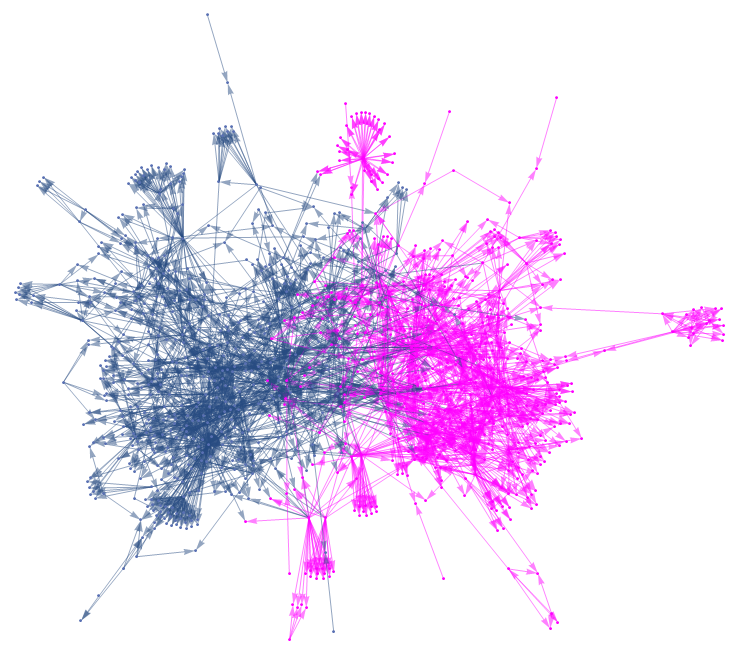
\includegraphics[width=0.9\textwidth]{subnetwork_partition.png}
\caption{The two halves of our partition of the pruned network.}
\label{fig:partitioned_network}
\end{figure}

In the process of collecting relevant papers for our citation network, we noticed that network similarity applications seem to be almost exclusively found in the fields of biology and computer science. We would therefore like to investigate the structure of the network with respect to these two categories. 

%\footnote{While the ``computer science" papers in our reading list all fall into the category of ``pattern recognition", this is not necessarily the case for their references, and we therefore use the broader label in our subject tagging process. Similarly, we use ``biology" instead of ``systems biology" when describing our category labels.}

Unfortunately, the metadata for the papers in our network does not include the subject information we would need to simply partition the network with respect to these categories. While the CrossRef API does sometimes include a ``subject" category, it is present in less than 1\% of items, and with almost six thousand references in our database, it is impractical to categorize their subjects by hand. Instead, we partition the network into two categories of equal size. If we choose our partition in a way that minimizes the fraction of edges running between its two groups (i.e., a modularity maximizing partition), it will preserve and separate the two clusters of more densely connected vertices first observed in Figure \ref{fig:pruned_network}, as we can see in Figure \ref{fig:partitioned_network}. We now attempt to determine whether these two halves of the network correspond to the two fields of application we noticed while constructing the dataset.

To do so, we need some way to roughly tag papers by their subject. We chose to do this according to their journal(s) of publication, since this information is available for over 97\% of the papers in our network\footnote{Journal information was not manually corrected for the papers for which the CrossRef API returned an incorrect result. However, in the vast majority of those cases, the result returned was very similar to the correct one--i.e., written by most of the same authors, or an older paper on the same subject. The subject information should therefore still be accurate enough for our purposes.}. There were a total of 2,285 unique journal names, which we tagged as ``Computer Science", ``Biology", and ``Mathematics" according to the keywords listed in Table \ref{tab:tagging_keywords}. This strategy allowed us to quickly tag the majority of the papers with at least one of these three subjects.

Our journal-based tagging is a drastic improvement over the subject information provided by CrossRef, giving us information for about 67\% of the total papers and 53\% of those in the pruned network. We found this to be sufficient to confirm our initial suspicions that the two communities observed in the network do in fact correspond to the fields of computer science (primarily pattern recognition) and systems biology. In the remainder of this chapter, we show how these categories are reflected in the structure of the dataset both overall and with respect to our partition, and then discuss the advantages that our dataset and analysis provide in our reading and writing process.

\begin{figure}[p]
\centering
\begin{minipage}[c]{0.23\textwidth}
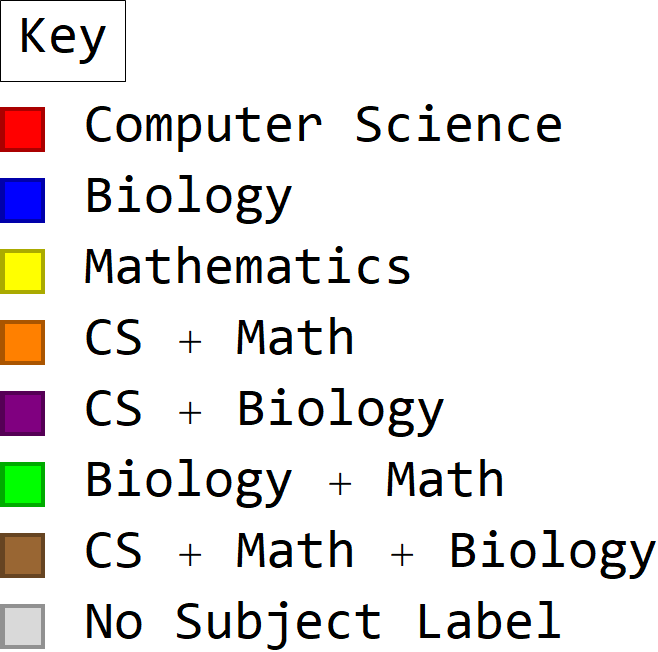
\includegraphics[width=\textwidth]{color_key.png}
\end{minipage}
\hfill
\begin{minipage}[c]{0.7\textwidth}
a)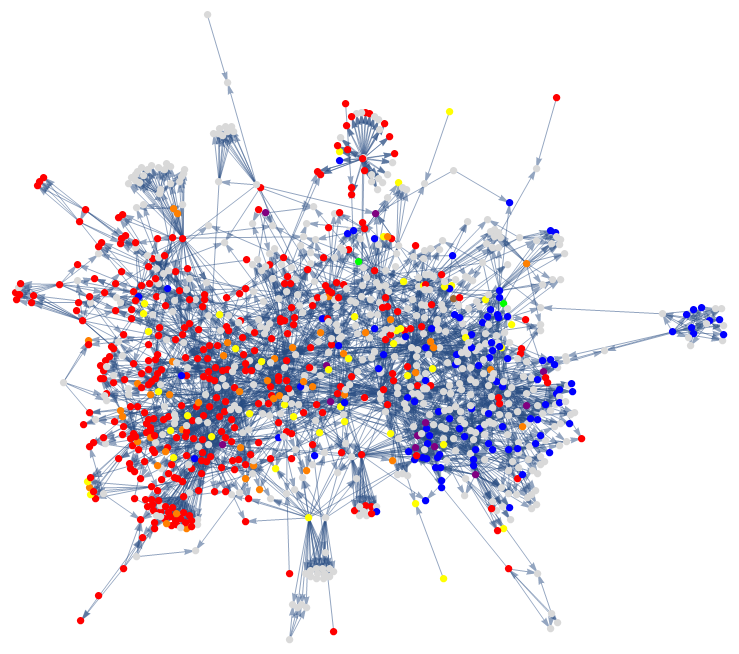
\includegraphics[width=\textwidth]{color_coded_full.png}
\end{minipage}
\begin{minipage}[c]{0.49\textwidth}
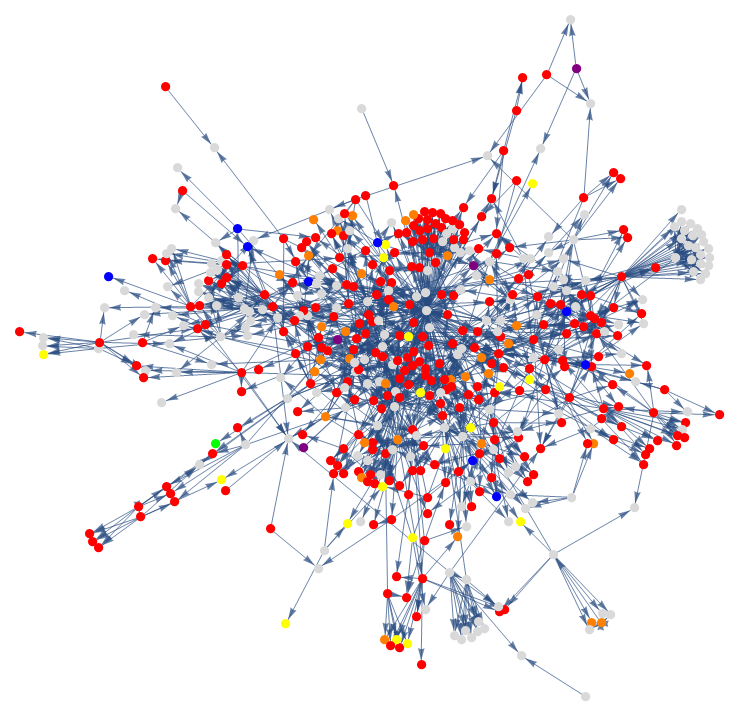
\includegraphics[width=0.95\textwidth]{color_coded_left.png}

b)
\vspace{-16pt}
\end{minipage}
\hfill
\begin{minipage}[c]{0.49\textwidth}
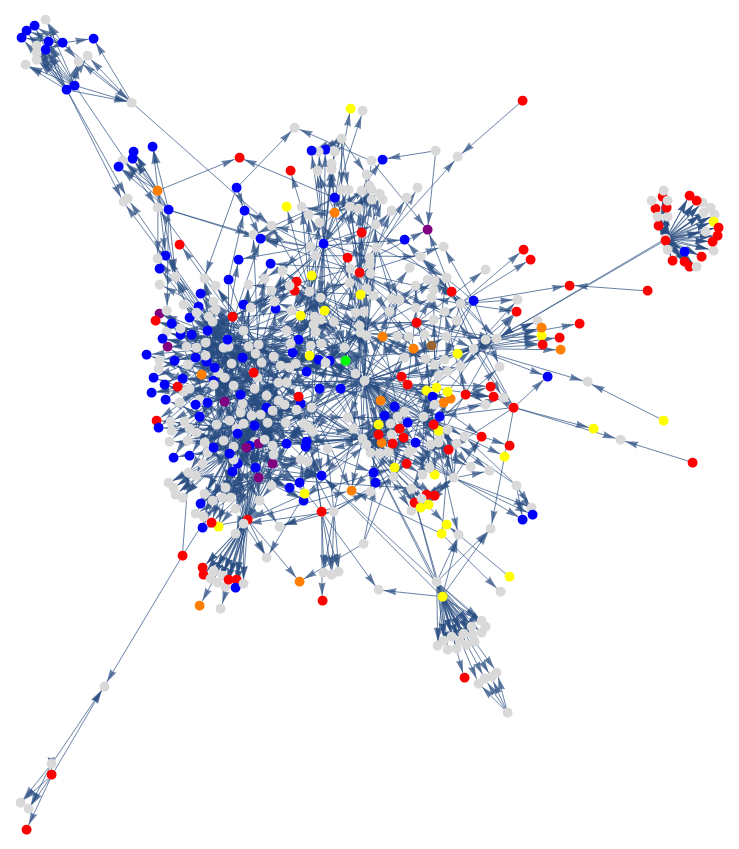
\includegraphics[width=0.95\textwidth]{color_coded_right.png}
\end{minipage}
\caption{a) The pruned network $G_p$, and b) the two halves of its partition $G_p^{(1)}$ and $G_p^{(2)}$, with vertices colored according to their subject label.}
\label{fig:subject_color_coded}
\end{figure}








\section{Results}

Our first step is to color code the vertices in the pruned network according to their subject, as shown in Figure \ref{fig:subject_color_coded}, so we can get a visual sense of how our tagged subjects are spread through the network. We then count the number of vertices in each color-coded category, as shown in Table \ref{tab:subject_counts}. While the main two categories we are interested in are computer science (red) and biology (blue), we have also tagged the mathematics papers (yellow) in order to obtain a third category of similar size and generality to the other two. This serves as a control group and allows us to consider and reject the hypothesis that there are three main subnetworks of similar papers instead of two. 

Visually, we can see that the red (CS) and blue (biology) vertices are mostly clustered together on the two halves of the pruned network, confirming our suspicion that the two dense clusters of vertices we see in Figure \ref{fig:pruned_network} correspond to the two categories we observed while constructing the dataset. Counting the tagged vertices supports this conclusion; there are 312 CS papers in $G_p^{(2)}$ but only 93 in $G_p^{(1)}$, and there are 108 biology papers in $G_p^{(1)}$ but only 14 in $G_p^{(2)}$. We also notice in Figure \ref{fig:subject_color_coded}b that the cluster of blue vertices only fills about half of its side of the partition, indicating that the biology category is significantly smaller than the computer science category; this is supported by the fact that there are 405 vertices tagged as CS in $G_p$, but only 122 tagged as biology. The yellow (math) is about evenly spread across the two halves (44 vs. 53), meaning that we do not have three distinct meaningful subnetworks of papers. 

There are also significantly more untagged vertices on the biology side of the partition (311 vs. 191). It is likely that this is not only because the computer science category is inherently larger, but because its papers are more likely to be tagged as such. A full half of the papers in the computer science category are published in an ACM, IEEE, or SIAM journal\footnote{Both ``SIAM" and ``algorithm" were used as keywords for both math and computer science, which accounts for about half of the overlap between the two categories. IEEE journals alone represent 35\% of the CS-tagged papers.}, all of which are easily tagged using these acronyms as a keyword. There were not any analagous dominant organizations with acronym keywords for the biology journals in our dataset, so the tagging relies on topical keywords and therefore can identify fewer of the biology papers with a reasonable number of keywords in our search. As a result, the computer science network is more strongly identified as such, and therefore more structurally visible to the partitioning algorithm.

\begin{table}[t]
\centering
\setlength\extrarowheight{3pt}
\begin{tabular}{|l|r|r|r|r|}
\hline & $G$ & $G_p$ & $G_p^{(1)}$ & $G_p^{(2)}$ \\ \hline\hline
Total vertices & 5793 & 1062 & 531 & 531 \\ \hline
Untagged & 1922 & 502 & 311 & 191 \\ \hline
Tagged & 3871 & 560 & 220 & 340 \\ \hline
CS & 2533 & 405 & 93 & 312 \\ \hline
Biology & 984 & 122 & 108 & 14 \\ \hline
Math & 787 & 97 & 44 & 53 \\ \hline
Both CS and biology & 108 & 13 & 9 & 4 \\ \hline
Both CS and math & 305 & 49 & 15 & 34 \\ \hline
Both biology and math & 24 & 3 & 2 & 1 \\ \hline
All three & 4 & 1 & 1 & 0 \\ \hline
\end{tabular}
\caption{Number of vertices tagged as computer science, biology, math, or some combination of these in $G$, $G_p$, and the two halves of the partition $G_p^{(1)}$ and $G_p^{(2)}$.}
\label{tab:subject_counts}
\end{table}

Color codings for the full network and the subnetwork of high centrality papers can be found in Figures \ref{fig:full_subject_color_coded} and \ref{fig:reading_list_subject_colored}, and a table of vertex counts similar to Table \ref{tab:subject_counts} for the high centrality subnetwork can be found in Table \ref{tab:reading_list_subject_counts}.

\subsection{Assortativity results}

\begin{table}[h]
\centering
\setlength\extrarowheight{3pt}
\begin{tabular}{|l|r|r|}
\hline
 & $G$ & $G_p$ \\ \hline\hline
Outdegree & -0.0178 & -0.0141 \\ \hline
Publication year & 0.0067 & 0.0041 \\ \hline
Citation count & 0.0006 & 0.0654 \\ \hline
Reference count & 0.0193 & -0.0061 \\ \hline
Tagged with any subject & 0.1089 & -0.0094 \\ \hline
Subject & 0.1837 & 0.0712 \\ \hline
Subject is CS & 0.2624 & 0.1529 \\ \hline
Subject is biology & 0.3354 & 0.1773 \\ \hline
Subject is math & 0.0732 & 0.0164 \\ \hline
Subject is CS or biology & 0.1500 & 0.0188 \\ \hline
Subject is CS or math & 0.2458 & 0.1256 \\ \hline
Subject is biology or math & 0.1713 & 0.0414 \\ \hline
\end{tabular}
\caption{Assortativity of the full and pruned citation networks with respect to various network properties.}
\label{tab:assortativity}
\end{table}

We would like to calculate the assortativity\footnote{According to the definition used by Mathematica's GraphAssortativity function.} of the network with respect to our subject tagging in order to measure the degree to which papers on a certain topic cite other papers on the same topic. It is unclear how to do so, however, since our vertices can belong to multiple categories, while the assortativity algorithm requires categories to be exclusive. To handle this issue, we report results in Table \ref{tab:assortativity} with respect to multiple strategies for dealing with multiple category membership. We can either define category intersections to be their own, separate category, which was the approach for the ``Subject" row in Table \ref{tab:assortativity}, or we can calculate assortativity with respect to whether a vertex is or is not tagged as a certain subject or group of subjects, which was the approach for the ``Subject is --" lines in Table \ref{tab:assortativity}.

For non-subject properties, our assortativity values are all very low in absolute value, meaning that vertices are neither more nor less likely to cite vertices with similar outdegree, publication year, citation count, or reference counts as themselves than they are to cite those with different values for these statistics.

We do, however, notice nontrivial assortativity with respect to several of our subject-based properties. The values are much lower than what we observed for the example in Figure \ref{fig:assortativity_demo}, which had an assortativity of 0.72, but this is not surprising. Many of the papers on each of our topics could not be tagged as such, so the assortativity is not as high as it likely would be with perfect subject tagging. We also would not expect to see as much assortativity in the citation network of an interdisciplinary academic research area as we would in a network of non-academic political books, especially when there is significant overlap between our categories. Survey papers in particular will lower the assortativity as they draw connections between work on a similar topic in different disciplines.

We first notice that the assortativity values in $G_p$ are lower than their corresponding values in all of $G$. That is, the papers with only one parent (which we have removed in $G_p$) are more likely to have the same subject tag as their parent than those cited by multiple papers. We also observe that there is very little assortativity with respect to whether a paper's subject is mathematics, which justifies our hypothesis that the assortativity with respect to computer science and biology is noteworthy and not something observed in any subject classification.

Finally, we note that the assortativity with respect to whether a paper is either computer science or biology is much lower than with respect to either category on its own and only somewhat higher than the assortativity with respect to whether a paper is tagged at all. The assortativity with respect to whether a paper is computer science or math is only slightly lower than with respect to computer science by itself, while the assortativity with respect to whether a paper is computer science or biology is much lower than with respect to biology by itself. That is, the math category is more highly structurally linked to computer science than biology (which is unsurprising, given the relative sizes of its intersections with each category), and biology is the most structurally distinct category overall. 








\section{How centrality and context inform a better survey}

In Section \ref{section:high_centrality_vertices}, we introduced a collection of 61 papers which were found to have high centrality either overall or within one of the sides of our partition of the pruned network. Our goal is to frame our presentation around the most important papers in the network, so they form our primary reading list. 

To facilitate our reading, we collected and tabulated metadata for the high centrality papers, including their author, year, title, DOI number, whether they are a parent in the network, their rank with respect to each of our centrality metrics overall and within each side of the partition, and their overall rank as discussed in Section \ref{section:high_centrality_vertices}. We also considered the subnetwork of our high centrality vertices, which we refer to as $G_R$, and visually organized them as shown in Figure \ref{fig:reading_list} and Figure \ref{fig:reading_list_neighborhood} to allow us to see at a glance the context of each paper in the wider reading list. We can also count how many vertices in each paper's neighborhood within $G_R$ fall on either side of the partition, which we can use as a guide to which papers might be highly interdisciplinary either in the references they cite or the papers they are cited by. Finally, we can use the Mathematica representation of the network to easily calculate how many and which of a paper's references are in the pruned network and on either side of the partition or to check the intersection of the neighborhoods of two or more papers.

\begin{sidewaysfigure}
\centering
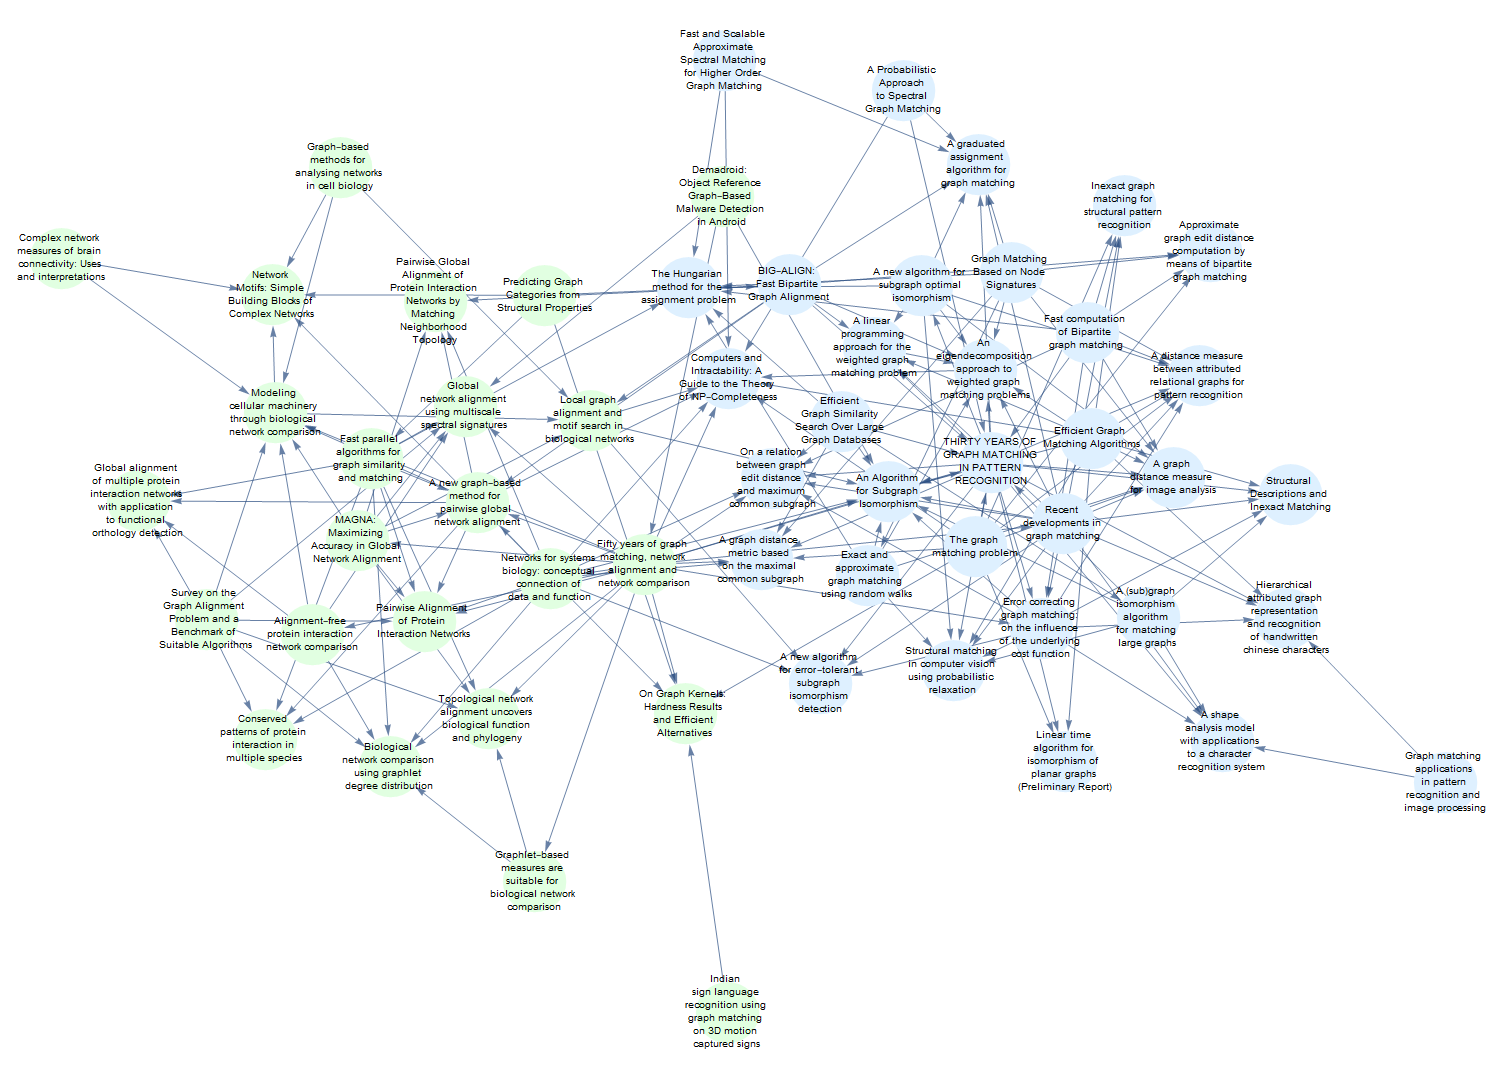
\includegraphics[width=0.85\textwidth]{reading_list0pt9crop.png}
\caption{The subnetwork $S$ of high centrality papers, as listed in Tables \ref{tab:toppapers_all}, \ref{tab:toppapers_bio}, and \ref{tab:toppapers_CS}. Green vertices are in the biology-dominated side of the partition of $G_p$, and blue vertices are in the CS-dominated side.}
\vspace{-12pt}\flushleft\scriptsize Note: ``Unsupervised Domain Adaptation Using Regularized Hyper-Graph Matching" is not in the connected component and is not displayed.
\label{fig:reading_list}
\end{sidewaysfigure}

\begin{sidewaysfigure}
\centering
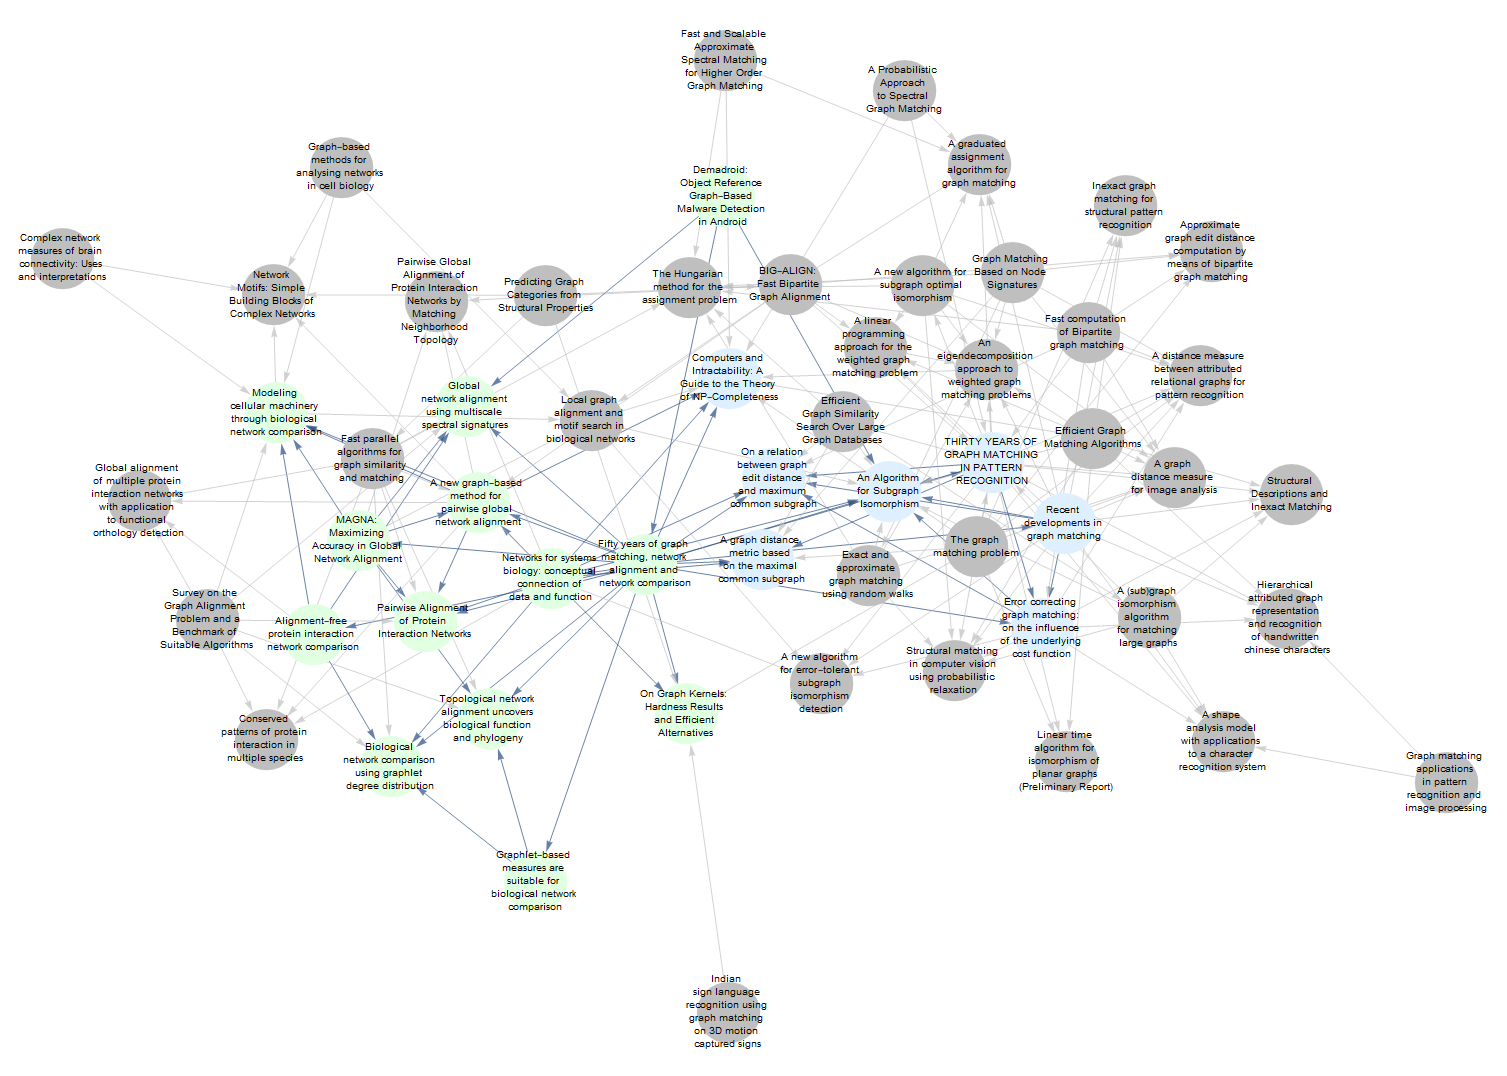
\includegraphics[width=0.85\textwidth]{reading_list_neighborhood0pt9crop.png}
\caption{The neighborhood of ``Fifty years of graph matching, network alignment, and network comparison" \cite{Emmert_Streib_2016} within the subnetwork $S$ of high centrality papers.}
\vspace{-12pt}\flushleft\scriptsize Note: ``Unsupervised Domain Adaptation Using Regularized Hyper-Graph Matching" is not in the connected component and is not displayed.
\label{fig:reading_list_neighborhood}
\end{sidewaysfigure}

At this point, we have a powerful amount of context to guide our reading. We know that there are two main categories of application in our dataset, we know roughly how they inform its structure, and we know which papers are important in each category as well as overall. We know that we are only reading papers which are considered important in some way, we know that they are important within our topic of interest specifically, and we know exactly \textit{how} important they are considered to be in comparison to the rest and why. 

As we read, we can easily check a paper's neighbors against those we have already read to place it within the context of the overall shape of the field and to compare our computational insights into which of the references included are relevant with the author's choices in how to frame them. We can choose to start by reading the papers with high authority centrality (in order to gain an understanding of concepts before building upon them) and then follow both year and forward reference information to track the development of the field over time. We can check for connections in the form of cocitations between papers we might expect to be connected based on the ideas they discuss--which is interesting both when the connections are there and when they are not--and thereby get a sense of the idea transfer between the two disciplines; which ideas have found crossover, which ideas have not, and why. 

Overall, we acquire a global sense of the shape of the field of network similarity which we can trust to be less biased by our own or other author's perceptions of what is important. At this point, it is easy to choose additional papers to read and refer to as needed throughout the reading and writing process and to use their reference lists to put them in the context of our existing understanding. As a last remark, we note that our context is based largely on the reading list subnetwork alone--which was formed using an arbitrary cutoff of ``top ten papers"--and that the network mathematics involved is quite basic. As helpful as we have found this context to be, we have likely only scratched the surface of the possible benefits of this method of exploration.

In the next two chapters, we outline the motivation and approach for our two main categories of application, starting with pattern recognition in Chapter \ref{chapter:pattern_recognition} and then discussing biology in Chapter \ref{chapter:systems_biology}.








%%%%%%%%%%%%%%%%%%%%%%%%%%%%%%%% CHAPTER 4 %%%%%%%%%%%%%%%%%%%%%%%%%%%%%%%%%%%%%%%







\chapter{Pattern Recognition}\label{chapter:pattern_recognition}
 
\section{Motivation}

The complex and combinatorial nature of graphs makes them computationally very difficult to work with, but it also makes them an incredibly powerful data structure for the representation of various objects and concepts. They are particularly useful in computer vision, where we would often like to recognize certain objects in an image (or across images) that seem different at the pixel level as a result of things like angles, lighting, and image scaling. Since graphs are invariant under positional changes including translations, rotations, and mirroring, they are well suited for this task.

Applications in the area of computer vision include optical character recognition \cite{Lu_1991,Rocha_1994}, biometric identification \cite{isenor1986fingerprint,deng2010retinal} and medical diagnostics \cite{sharma2012determining}, and 3D object recognition \cite{Christmas_1995}. In 2018, work has been published in the computer vision-related areas of Indian sign language recognition \cite{Kumar_2018a,Kumar_2018b}, spotting subgraphs (e.g., certain characters) in comic book images \cite{le2018ssgci}, and stacking MRI image slices \cite{clough2018mri}. A timeline with more comprehensive counts of papers in various application areas of pattern recognition through 2002 can be found in \cite{Conte_2004}.

\begin{figure}[t!]
\centering
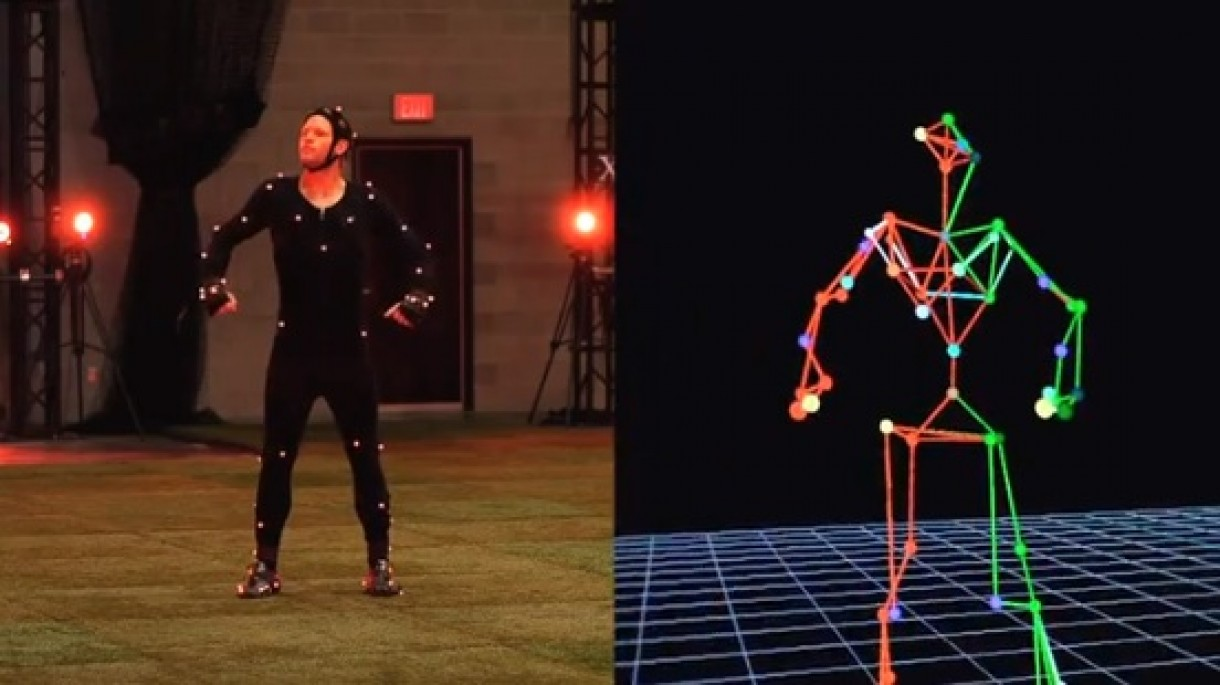
\includegraphics[width=\textwidth]{motion_capture_demo.png}
\scriptsize Source: http://ultimatefifa.com/2012/fifa-13-motion-capture-session/
\caption{A graph-based representation of a human body, with nodes corresponding to the markers on a motion capture suit.}
\label{motion_capture_demo}
\end{figure}

In computer vision applications, we can create a graph representation for an image by decomposing it into parts and using edges to represent the relationships between these components. For example, we can describe a person using the relationships between various body parts: head, shoulders, knees, toes, and so on. This is the idea behind motion capture, as illustrated in Figure \ref{motion_capture_demo}. After we have a graph representation of the objects we would like to compare, the problem of recognition--and in particular the problem of database search--is reduced to a graph matching problem. To find an object in a database, we must compare its graph representation to a database of model graphs to determine which is the most similar.








\section{Graph matching}\label{section:defining_graph_matching}

In the literature, the term ``graph matching"\index{graph matching} is used significantly more often than it is explicitly defined. When a definition is given, it is usually tailored to the purposes of a particular author, and specific to a certain type of graph matching; i.e., exact, inexact, error-correcting, bipartite, and so on. The distinctions between these can be subtle, and are typically only explicitly addressed in survey papers. Furthermore, we sometimes address the question of finding a matching \textit{in} a graph \cite{wikiMatchingInAGraph}\index{matching in a graph}, which is different from but still related to the problem of graph matching, in which we want to find a mapping \textit{between} two graphs. And finally, there is a significant presence in the literature of \textit{elastic} graph matching\index{elastic graph matching}, which is widely used in pattern recognition but is not in fact a form of graph matching \cite{Conte_2003}. Clearly a good taxonomy is needed. In this section, we give an overview of graph matching-related terms and summarize their distinctions.

\subsection{Preliminary definitions}

Graph isomorphism is the strictest form of graph matching and a natural place to begin our discussion. We now define graph isomorphism and two relevant generalizations of the graph isomorphism problem (see Figure \ref{fig:isomorphism_demos} and Table \ref{NP_classifications}), as well as the temporal complexity terms necessary to compare their computational difficulty.

A decision problem (i.e., one which can be posed as a yes or no question), of which the graph isomorphism problem is an example, is in \textbf{NP}\index{NP} or \textbf{nondeterministic polynomial time} if the instances where the answer is ``yes" can be verified or rejected in polynomial time \cite{Hartmanis_1982,wikiNPComplexity}. It is \textbf{NP-hard}\index{NP-hard} if it is ``at least as difficult as every other NP problem"; that is, every problem which is in NP can be reduced to it in polynomial time. An NP-hard problem does not necessarily have to be in NP itself  \cite{Hartmanis_1982,wikiNPHardness}. If a decision problem is both NP and NP-hard, it is \textbf{NP-complete}\index{NP-complete} \cite{Hartmanis_1982,wikiNPCompleteness}.

An \textbf{induced subgraph}\index{induced subgraph} of a graph is a graph formed from a subset of nodes in the larger graph and all the edges between them \cite{wikiInducedSubgraph}. By contrast, a \textbf{subgraph}\index{subgraph} is simply a graph formed from a subset of the nodes and edges in the larger graph \cite{wikiSubgraph}.

\begin{figure}[!t]
\centering
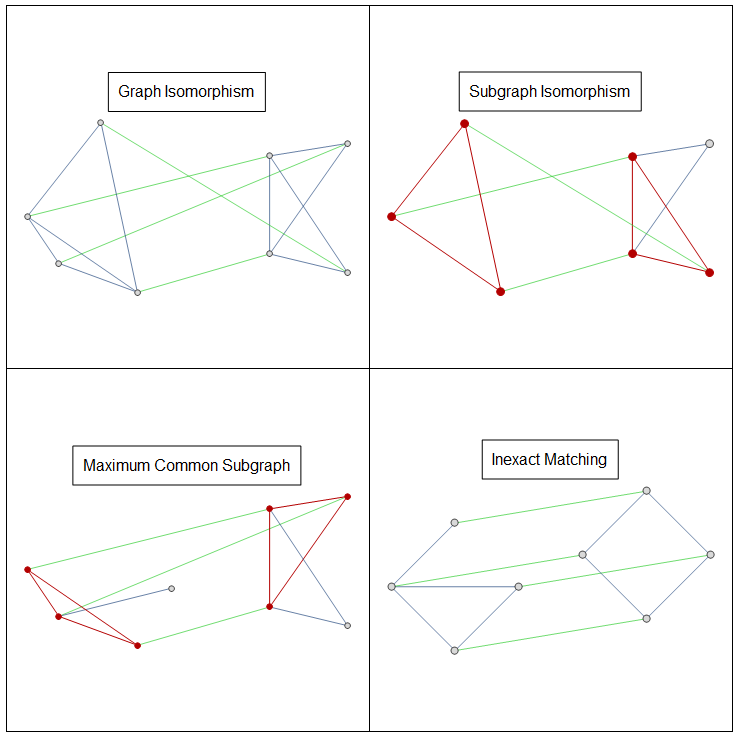
\includegraphics[width=\textwidth]{isomorphism_demos.png}
\caption{A visual summary of the distinctions between graph isomorphism, subgraph isomorphism, maximum common subgraph, and inexact matching.}
\label{fig:isomorphism_demos}
\end{figure}

A \textbf{graph isomorphism}\index{graph isomorphism} is a bijective mapping between the nodes of two graphs of the same size which is \textbf{edge-preserving}\index{edge-preserving}; that is, if two nodes in the first graph are connected by an edge, they are mapped to two nodes in the second graph which are also connected by an edge \cite{Conte_2004}. The decision problem of determining whether two graphs are isomorphic is neither known to be in NP nor known to be solvable in polynomial time \cite{wikiGraphIsomorphism}.

A \textbf{subgraph isomorphism}\index{subgraph isomorphism} is an edge-preserving injective mapping from the nodes of a smaller graph to the nodes of a larger graph. That is, there is a subgraph isomorphism between two graphs if there is an isomorphism between the smaller graph and some induced subgraph of the larger \cite{Conte_2004}. The decision problem of determining whether a graph contains a subgraph which is isomorphic to some smaller graph is known to be NP-complete \cite{wikiSubgraphIsomorphism}.

Finally, a \textbf{maximum common induced subgraph}\index{maximum common subgraph} (MCS) of two graphs is a graph which is an induced subgraph of both and has as many nodes as possible  \cite{wikiMaximumCommonSubgraph}. Formulating the MCS problem as a graph matching problem can be done by defining the metric \[d(G_1,G_2) = 1 - \frac{|\text{MCS}(G_1,G_2)|}{\max\{|G_1|,|G_2|\}},\] where $|G|$ is the number of nodes in $G$ \cite{Bunke_1998,Bunke_1997}.

\begin{table}[t!]
\centering
\setlength\extrarowheight{3pt}\setlength{\tabcolsep}{6pt}
\begin{tabular}{|L{0.3\linewidth}|C{0.14\linewidth}|C{0.14\linewidth}|C{0.21\linewidth}|}
\hline
 & Graph isomorphism & Subgraph isomorphism & Maximum common induced subgraph \\ \hline\hline
$G_1$ and $G_2$ must have the same number of nodes & X & & \\ \hline
Mapping must include all nodes of either $G_1$ or $G_2$ & X & X & \\ \hline
Mapping must be edge-preserving & X & X & X\hspace{6pt} \\ \hline
NP-complete & Unknown & X & X$^*$ \\ \hline
\end{tabular}
\flushleft\footnotesize *The associated decision problem of determining whether $G_1$ and $G_2$ have a common induced subgraph with at least $k$ nodes is NP-complete, but the problem of finding the maximum common induced subgraph (as required for graph matching) is NP-hard \cite{wikiMaximumCommonSubgraph}.
\caption{A summary of exact graph matching problem formulations.}
\label{NP_classifications}
\end{table}

\subsection{Exact and inexact matching}\label{section:exact_and_inexact_matching}

\begin{table}[t!]
\centering
\setlength\extrarowheight{3pt}\setlength{\tabcolsep}{2.5pt}
\begin{tabular}{|L{0.16\linewidth}|C{0.19\linewidth}|C{0.11\linewidth}|C{0.195\linewidth}|C{0.105\linewidth}|C{0.165\linewidth}|}
\hline
 & Edge preserving? & Result in? & Mapping seeking? & Optimal? & Complexity \\ \hline\hline
Graph isomorphism & Yes & \{0,1\} & Yes & Yes & Likely between P and NP \\ \hline
Subgraph isomorphism & Yes & \{0,1\} & Yes & Yes & NP-complete \\ \hline
MCS computation & Yes & [0,1] & Yes & Yes & NP-hard \\ \hline
Edit distances (exact) & No & [0,1] & No & Yes & Generally exponential \\ \hline
Edit distances (approximate) & No & [0,1] & No & No & Generally polynomial \\ \hline
Other inexact formulations & No & [0,1] & Sometimes & No* & Generally polynomial \\ \hline
\end{tabular}
\caption{Summary of the distinctions between exact and inexact graph matching styles.}
\vspace{-8pt}
\flushleft\footnotesize *The Hungarian algorithm can be used to find an optimal assignment in $O(n^3)$ time based on a given cost function, but the assignment problem minimizes a cost function which is only an approximation of the true matching cost.
\label{exact_vs_inexact}
\end{table}

We define a graph matching method to be \textbf{exact}\index{exact matching} if it seeks to find a mapping between the nodes of two graphs which is edge preserving. Exact matching is also sometimes defined by whether a method seeks a boolean evaluation of the similarity of two graphs \cite{Livi_2012,Emmert_Streib_2016}. For graph and subgraph isomorphism, this characterization is equivalent; either two graphs are isomorphic, or they are not. Since the maximum common subgraph problem is edge preserving, we consider it in this work to be an exact matching problem. However, it does not seek a boolean evaluation, and it is therefore sometimes considered to be an inexact matching problem \cite{Livi_2012}. 

In \textbf{inexact matching}\index{inexact matching}, we also search for mappings which are not edge-preserving. This allows us to compensate for the inherent variability of the data in an application, as well as the noise and randomness introduced by the process of constructing graph representations of that data. Instead of matchings between nodes being forbidden if edge-preservation requirements are unsatisfied, they are simply penalized in some way. We then seek to find a matching that minimizes the sum of this penalty cost. Instead of returning a value in $\{0,1\}$, we return a value in $[0,1]$ measuring the similarity or dissimilarity between two graphs\footnote{Returning 1 for an isomorphism is analagous to a boolean evaluation and would be considered a similarity measure. Most algorithms for inexact matching seek to minimize some function, so they would return 0 for an isomorphism and are therefore considered \textit{dis}similarity measures.}.

Inexact matching algorithms which are based on an explicit cost function or edit distance are often called \textbf{error tolerant}\index{error tolerant} or \textbf{error correcting}\index{error correcting}. 

\subsubsection{Optimal and approximate algorithms}

Problem formulations for inexact matching generally seek to minimize some nonnegative cost function which should theoretically be zero for two isomorphic graphs. An \textbf{optimal}\index{optimal algorithm} algorithm is one which is guaranteed to find a global minimum to this cost function; it will find an isomorphism if it exists, but it still handles the problem of graph variability. As a result, however, optimal algorithms for inexact matching are significantly more expensive than their exact counterparts \cite{Conte_2004}.

Most inexact matching algorithms are therefore \textbf{approximate}\index{approximate algorithm} or \textbf{suboptimal}\index{suboptimal algorithm}. They only find a local minimum of the cost function (either by optimizing it directly, or approximating it by some other cost function), which may or may not be close to the true minimum. This may or may not be acceptable in a certain application, but it allows these algorithms to be much less expensive to calculate--usually polynomial time  \cite{Conte_2004}.

\subsubsection{Mapping-seeking and non-mapping-seeking algorithms} 

Finally, we can draw the distinction of whether the algorithm seeks primarily to find a mapping between nodes (and returns a result in $\{0,1\}$ or $[0,1]$ as a byproduct of the mapping if it does so at all), or whether it does not. All exact formulations seek a mapping, and many inexact formulations do as well. Mapping-seeking inexact matching is more commonly referred to as \textbf{alignment}\index{alignment} and is one of two overwhelmingly dominant comparison strategies in biological applications. Alignment is discussed in more detail in Chapter \ref{chapter:systems_biology}.

\subsection{Graph kernels and embeddings}

``The Graph Matching Problem" \cite{Livi_2012}, published in 2012, claims that there are three main approaches to the inexact graph matching problem: edit distances, graph kernels, and graph embeddings. We did not observe this to be the case in our reading, but we still give a brief introduction to graph kernels and embeddings and discuss our observations.

Graph \textbf{embeddings}\index{graph embedding} map a graph into some high-dimensional feature space, allowing us to perform comparisons there \cite{Emmert_Streib_2011}. For example, we could identify a graph with a vector in $\R^n$ containing the seven statistics reported in Table \ref{tab:network_table} or the eigenvalues of its adjacency matrix and then compare them using the Euclidean distance. Mapping a graph into Euclidean space certainly makes comparison easier, but it is not obvious how to create a mapping that preserves graph properties in a sensible way. Graph statistics and embeddings must be shown experimentally to be useful; they may allow us to distinguish between different classes of graphs, correlate with some other desirable property, narrow down matching candidates in a large database (allowing them to be used for hashing), and so on.
\newpage

Graph \textbf{kernels}\index{graph kernel} are a special kind of graph embeddings in which we have a continuous map $k:\mathcal{G}\times \mathcal{G}\rightarrow \R$, where $\mathcal{G}$ is the space of all possible graphs, such that $k$ is symmetric and positive definite or semidefinite \cite{Livi_2012}. Creating a kernel for graphs would allow us to take advantage of the techniques and theory of general kernel methods, but it has been shown that computing a strictly positive definite graph kernel is at least as hard as solving the graph isomorphism problem \cite{Gartner_2003}. We suspect that the amount of work involved in creating a (not necessarily strictly positive definite) graph kernel with enough desirable properties to take advantage of kernel methods is prohibitive enough in many cases to make this an impractical strategy.

We note that the strategy of using the graphlet degree distribution\index{graphlet degree distribution}, which we discuss in Chapter \ref{chapter:systems_biology}, is a form of embedding. Furthermore, the graph kernel strategies described in the references of  \cite{Livi_2012} seem to use the assignment problem-style approach of calculating some sort of similarity notion between pairs of nodes in two graphs and then using that matrix to create the desired alignment or kernel. We therefore consider the strategies of graph kernels and graph embeddings to be part of the families of other categories which we describe in this work rather than mainstream approaches in their own right.








\section{Exact matching and graph edit distance}

The field of graph matching is large and well-established, and we cannot hope to give a full overview of all existing techniques without sacrificing our focus on remaining accessible to the relative novice. If the reader is interested in a more comprehensive investigation, the definitive\footnote{This is clear from the way it is discussed by later works, but it also has the highest indegree, outdegree, betweenness ranking, and HITS hub ranking in our pruned network, and is second for closeness.} source on graph matching developments through 2004 is ``Thirty Years of Graph Matching In Pattern Recognition" \cite{Conte_2004}. Two of its authors collaborated with various others on a similar survey in 2014 covering the ten years since the prior survey's publication \cite{foggia2014graph} and in June of 2018 published a large-scale performance comparison of graph matching algorithms on huge graphs \cite{carletti2018comparing} that may also be of interest.

We partition the field into three general approaches: 

\begin{enumerate}
\item Exact matching methods.
\item Edit distance-based methods for optimal inexact matching. 
\item Continuous optimization-based methods for inexact matching. 
\end{enumerate}

We present optimization methods in their own section and network alignment and comparison methods in Chapter \ref{chapter:systems_biology}. In this section, we introduce the concepts of search space pruning (the most dominant approach for exact matching), a graph edit path, and its corresponding graph edit distance. Our presentation of edit distances is primarily inspired by \cite{Livi_2012} and \cite{Riesen_2009}.

\subsection{Search space pruning}\index{search space pruning}

Most algorithms for exact graph matching are based on some form of tree search\index{tree search} with backtracking \cite{Conte_2004}. The process is analagous to solving a grid-based logic puzzle: we represent all possible matching options in a grid format and then rule out infeasible possibilities based on clues or heuristics about the problem. When we get to the point where our clues can no longer rule out any further possibilities, we arbitrarily choose one of the remaining possible options for a certain item. This rules out other possibilities, allowing us to use our clues again. We continue this process until we either complete the puzzle or reach a state where there are no possible solutions remaining. In the latter case, we backtrack, rule out our initial arbitrary choice, and try its alternatives until we either find a solution or exhaust all possible choices. The backtracking process is a depth-first search of the tree of possible mappings; our clues allow us to skip over branches without searching them.

The seminal algorithm for exact matching is found in Ullmann's 1976 paper ``An Algorithm for Subgraph Isomorphism" \cite{Ullmann_1976} and is applicable to both graph and subgraph isomorphism. We assume two graphs $g_1$ and $g_2$ with node counts $m$ and $n$, respectively, and assume without loss of generality that $m\leq n$. This allows us to represent all matching candidate possibilities in a $m\times n$ matrix of zeros and ones.

\newpage

The Ullmann algorithm\index{Ullmann subgraph isomorphism algorithm}\index{subgraph isomorphism} uses two principles to rule out matching possibilities:

\begin{enumerate}
\item We cannot map a node in $g_1$ to one in $g_2$ that has fewer neighbors. We use this principle to rule out matching possibilities initially. In Example \ref{ex:ullmann}, degree comparison reduces the number of possible matchings from $8^4=4096$ to $5^*5^*1^*8=200$. This drastic improvement comes at the cost of only $mn$ operations (comparing the degrees of each node in $g_1$ against each node in $g_2$).

\item We cannot map a node $v_1\in g_1$ to a node $v_2\in g_2$ unless all its neighbors have feasible matching possibilities among the neighbors of $v_2$. Testing this is called the \textbf{refinement}\index{refinement} procedure, and it forms the heart of the algorithm. In Example \ref{ex:ullmann}, after a single stage of the refinement process and before we begin backtracking we have reduced the number of possible matchings down to $3^*3^*1^*3=27$.
\end{enumerate}


\begin{example}\label{ex:ullmann}

Ullmann's presentation of his own algorithm is not intuitive. To illustrate his method, we step through an example found on StackOverflow \cite{ullmannStackOverflow}, where we determine whether a subgraph isomorphism exists between the graphs $g_1$ and $g_2$ shown below.


\vspace{-30pt}
\begin{center}
\begin{tabular}{C{0.35\textwidth}C{0.6\textwidth}}
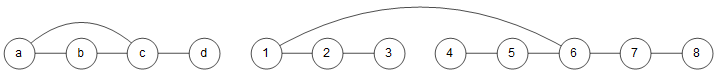
\includegraphics[width=0.95\textwidth]{ullmann_demo_cropped.png} & \\ $g_1$ & $g_2$\\
\end{tabular}
\end{center}

First, we use degree comparison to determine the initial candidates for mapping nodes in $g_1$ to nodes in $g_2$. Node $d$ has degree 1, so it can be mapped to anything in $g_2$. Nodes $a$ and $b$ have degree 2, so they cannot be mapped to nodes $3, 4$, or $8$ in $g_2$ as those nodes have degree 1. Finally, node $c$ has degree 3, so it can only be mapped to node 6.

\begin{center}
\begin{tikzpicture}
\matrix (m)[
    matrix of math nodes,
    nodes in empty cells,
    inner sep=4pt,
]{ 
 & 1 & 2 & 3 & 4 & 5 & 6 & 7 & 8 \\ \hline
a & 1 & 1 & 0 & 0 & 1 & 1 & 1 & 0 \\
b & 1 & 1 & 0 & 0 & 1 & 1 & 1 & 0 \\
c & 0 & 0 & 0 & 0 & 0 & 1 & 0 & 0 \\
d & 1 & 1 & 1 & 1 & 1 & 1 & 1 & 1 \\
};
\draw (m-5-2.south west) -- (m-1-2.north west);
\end{tikzpicture}
\footnotesize\singlespacing Candidate mapping pairs which satisfy degree requirements.
\end{center}
\vspace{-5pt}

Next, we begin the refinement procedure. We illustrate two cases of the refinement procedure for the candidates of node $a$ in $g_1$: one where the candidate is valid and another where it is not.

\vspace{-30pt}
\begin{center}
\begin{tabular}{C{0.35\textwidth}C{0.6\textwidth}}
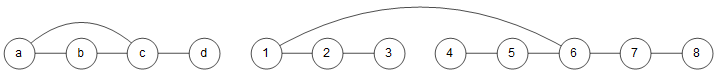
\includegraphics[width=0.95\textwidth]{ullmann_demo_cropped.png} & \\ $g_1$ & $g_2$\\
\end{tabular}
\end{center}

\begin{center}
\begin{minipage}{0.1\textwidth}
\hfill
\end{minipage}
\begin{minipage}{0.3\textwidth}
\begin{tikzpicture}
\matrix (m)[
    matrix of math nodes,
    nodes in empty cells,
    inner sep=4pt,
]{ 
 & 1 & 2 & 3 & 4 & 5 & 6 & 7 & 8 \\ \hline
a & 1 & 1 & 0 & 0 & 1 & 1 & 1 & 0 \\
b & 1 & 1 & 0 & 0 & 1 & 1 & 1 & 0 \\
c & 0 & 0 & 0 & 0 & 0 & 1 & 0 & 0 \\
d & 1 & 1 & 1 & 1 & 1 & 1 & 1 & 1 \\
};
\fill[gray,opacity=0.2] (m-3-1.south west) rectangle (m-3-9.north east);
\fill[gray,opacity=0.2]  (m-4-1.south west) rectangle (m-4-9.north east);
\fill[gray,opacity=0.2]  (m-5-3.south west) rectangle (m-1-3.north east);
\fill[gray,opacity=0.2]  (m-5-7.south west) rectangle (m-1-7.north east);
\draw (m-5-2.south west) -- (m-1-2.north west);
\draw[black,thick,radius=7pt] (m-2-2) circle;
\draw[green,thick,radius=7pt] (m-3-3) circle;
\draw[green,thick,radius=7pt] (m-4-7) circle;
\end{tikzpicture}
\footnotesize\singlespacing Node 1 is a suitable candidate for node $a$.
\end{minipage}
\begin{minipage}{0.1\textwidth}
\hfill
\end{minipage}
\begin{minipage}{0.3\textwidth}
\begin{tikzpicture}
\matrix (m)[
    matrix of math nodes,
    nodes in empty cells,
    inner sep=4pt,
]{ 
 & 1 & 2 & 3 & 4 & 5 & 6 & 7 & 8 \\ \hline
a & 1 & \cancel{1} & 0 & 0 & 1 & 1 & 1 & 0 \\
b & 1 & 1 & 0 & 0 & 1 & 1 & 1 & 0 \\
c & 0 & 0 & 0 & 0 & 0 & 1 & 0 & 0 \\
d & 1 & 1 & 1 & 1 & 1 & 1 & 1 & 1 \\
};
\fill[gray,opacity=0.2]  (m-3-1.south west) rectangle (m-3-9.north east);
\fill[gray,opacity=0.2]  (m-4-1.south west) rectangle (m-4-9.north east);
\fill[gray,opacity=0.2]  (m-5-2.south west) rectangle (m-1-2.north east);
\fill[gray,opacity=0.2] (m-5-4.south west) rectangle (m-1-4.north east);
\draw (m-5-2.south west) -- (m-1-2.north west);
\draw[black,thick,radius=7pt] (m-2-3) circle;
\draw[green,thick,radius=7pt] (m-3-2) circle;
\draw[red,thick,radius=7pt] (m-4-2) circle;
\draw[red,thick,radius=7pt] (m-4-4) circle;
\end{tikzpicture}
\footnotesize\singlespacing Node 2 is not a suitable candidate for node $a$.
\end{minipage}
\begin{minipage}{0.1\textwidth}
\hfill
\end{minipage}
\end{center}

\bigskip

On the left, we consider node 1 in $g_2$ as a candidate for node $a$ in $g_1$. We highlight the rows corresponding to $a$'s neighbors and the columns corresponding to 1's neighbors. Each neighbor of $a$ must have a candidate among the neighbors of 1; that is, there must be a 1 somewhere in the intersections of the highlighted columns with each highlighted row. Since this is the case on the left, 1 remains a candidate for $a$. On the right, however, we find that node 2 is not a valid candidate for $a$. While there is a candidate for $b$ among the neighbors of 2, there is not a candidate for $c$ among the neighbors of 2.

After performing the refinement process for all candidate pairings, the remaining candidates for each node in $g_1$ are as shown below. At this point, it is time to begin backtracking.

\vspace{5pt}
\begin{center}
\begin{tikzpicture}
\matrix (m)[
    matrix of math nodes,
    nodes in empty cells,
    inner sep=4pt,
]{ 
 & 1 & 2 & 3 & 4 & 5 & 6 & 7 & 8 \\ \hline
a & 1 & 0 & 0 & 0 & 1 & 0 & 1 & 0 \\
b & 1 & 0 & 0 & 0 & 1 & 0 & 1 & 0 \\
c & 0 & 0 & 0 & 0 & 0 & 1 & 0 & 0 \\
d & 1 & 0 & 0 & 0 & 1 & 0 & 1 & 0 \\
};
\draw (m-5-2.south west) -- (m-1-2.north west);
\end{tikzpicture}
\footnotesize\singlespacing Candidate mapping pairs after the initial refinement procedure.
\end{center}
\vspace{-5pt}

For the backtracking procedure, we try mapping a node to each of its candidates in turn. At each stage, if we cannot find any viable candidates for a node among the neighbors of the candidate in question, we backtrack and try again. The algorithm stops when we either find a subgraph isomorphism or eliminate all candidates for a node.

\vspace{-30pt}
\begin{center}
\begin{tabular}{C{0.35\textwidth}C{0.6\textwidth}}
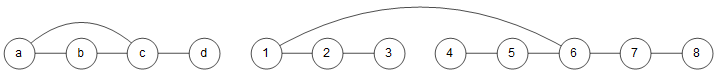
\includegraphics[width=0.95\textwidth]{ullmann_demo_cropped.png} & \\ $g_1$ & $g_2$\\
\end{tabular}
\end{center}
\begin{minipage}{0.3\textwidth}
\begin{center}
\begin{tikzpicture}
\matrix (m)[
    matrix of math nodes,
    nodes in empty cells,
    inner sep=4pt,
]{ 
 & 1 & 2 & 3 & 4 & 5 & 6 & 7 & 8 \\ \hline
a & \cancel{1} & 0 & 0 & 0 & 1 & 0 & 1 & 0 \\
b & 0 & 0 & 0 & 0 & 1 & 0 & 1 & 0 \\
c & 0 & 0 & 0 & 0 & 0 & 1 & 0 & 0 \\
d & 0 & 0 & 0 & 0 & 1 & 0 & 1 & 0 \\
};
\fill[gray,opacity=0.2]  (m-3-1.south west) rectangle (m-3-9.north east);
\fill[gray,opacity=0.2]  (m-4-1.south west) rectangle (m-4-9.north east);
\fill[gray,opacity=0.2]  (m-5-3.south west) rectangle (m-1-3.north east);
\fill[gray,opacity=0.2] (m-5-7.south west) rectangle (m-1-7.north east);
\draw (m-5-2.south west) -- (m-1-2.north west);
\draw[black,thick,radius=7pt] (m-2-2) circle;
\draw[green,thick,radius=7pt] (m-4-7) circle;
\draw[red,thick,radius=7pt] (m-3-3) circle;
\draw[red,thick,radius=7pt] (m-3-7) circle;
\end{tikzpicture}
\end{center}
\footnotesize\singlespacing Try mapping $a$ to $1$. There is no viable candidate for $b$ among the neighbors of $1$, so we backtrack and try again.
\end{minipage}\hfill
\begin{minipage}{0.3\textwidth}
\begin{center}
\begin{tikzpicture}
\matrix (m)[matrix of math nodes,inner sep=4pt
]{ 
 & 1 & 2 & 3 & 4 & 5 & 6 & 7 & 8 \\ \hline
a & 0 & 0 & 0 & 0 & \cancel{1} & 0 & 1 & 0 \\
b & 1 & 0 & 0 & 0 & 0 & 0 & 1 & 0 \\
c & 0 & 0 & 0 & 0 & 0 & 1 & 0 & 0 \\
d & 1 & 0 & 0 & 0 & 0 & 0 & 1 & 0 \\
};
\draw (m-5-2.south west) -- (m-1-2.north west);
\fill[gray,opacity=0.2]  (m-3-1.south west) rectangle (m-3-9.north east);
\fill[gray,opacity=0.2]  (m-4-1.south west) rectangle (m-4-9.north east);
\fill[gray,opacity=0.2]  (m-5-5.south west) rectangle (m-1-5.north east);
\fill[gray,opacity=0.2] (m-5-7.south west) rectangle (m-1-7.north east);
\draw[black,thick,radius=7pt] (m-2-6) circle;
\draw[green,thick,radius=7pt] (m-4-7) circle;
\draw[red,thick,radius=7pt] (m-3-5) circle;
\draw[red,thick,radius=7pt] (m-3-7) circle;
\end{tikzpicture}
\end{center}
\footnotesize\singlespacing Try mapping $a$ to 5. There is no viable candidate for $b$ among the neighbors of $5$, so we backtrack and try again.
\end{minipage}\hfill
\begin{minipage}{0.3\textwidth}
\begin{center}
\begin{tikzpicture}
\matrix (m)[matrix of math nodes,inner sep=4pt
]{ 
 & 1 & 2 & 3 & 4 & 5 & 6 & 7 & 8 \\ \hline
a & 0 & 0 & 0 & 0 & 0 & 0 & \cancel{1} & 0 \\
b & 1 & 0 & 0 & 0 & 1 & 0 & 0 & 0 \\
c & 0 & 0 & 0 & 0 & 0 & 1 & 0 & 0 \\
d & 1 & 0 & 0 & 0 & 1 & 0 & 0 & 0 \\
};
\draw (m-5-2.south west) -- (m-1-2.north west);
\fill[gray,opacity=0.2]  (m-3-1.south west) rectangle (m-3-9.north east);
\fill[gray,opacity=0.2]  (m-4-1.south west) rectangle (m-4-9.north east);
\fill[gray,opacity=0.2]  (m-5-9.south west) rectangle (m-1-9.north east);
\fill[gray,opacity=0.2] (m-5-7.south west) rectangle (m-1-7.north east);
\draw[black,thick,radius=7pt] (m-2-8) circle;
\draw[green,thick,radius=7pt] (m-4-7) circle;
\draw[red,thick,radius=7pt] (m-3-9) circle;
\draw[red,thick,radius=7pt] (m-3-7) circle;
\end{tikzpicture}
\end{center}
\footnotesize\singlespacing Try mapping $a$ to 7. There is no viable candidate for $b$ among the neighbors of $7$, and no more candidates for $a$, so we stop.
\end{minipage}

\vspace{15pt}

We cannot find a suitable candidate for $b$ among the neighbors of any candidate of $a$, so there is no subgraph isomorphism between $g_1$ and $g_2$.
\end{example}

\subsection{Graph edit distance}

\begin{wrapfigure}{R}{0.45\textwidth}
\centering
\begin{tabular}{|lcl|l|}
\hline
cat & $\rightarrow$ & ca\textit{r}t & Insertion \\ \hline
\textit{c}art & $\rightarrow$ & \textit{d}art & Substitution \\ \hline
\textit{d}art & $\rightarrow$ & art & Deletion \\ \hline
\textit{ar}t & $\rightarrow$ & \textit{ra}t & Transposition \\ \hline
\end{tabular}
\caption{Edit operations for strings.}
\label{fig:string_edit_operations}
\end{wrapfigure}

One way to measure the distance between two objects is to measure how much work it takes to turn the first into the second, and take the length of the \textbf{edit path}\index{edit path}. For example, in Figure \ref{fig:string_edit_operations}, we find an edit path of length 4 between ``cat" and ``rat". However, this should clearly not be the edit distance\index{graph edit distance} between ``cat" and ``rat", as we can transform one into the other with a single substitution. The \textbf{edit distance} between two objects is therefore the \textit{minimum} over the lengths of all possible edit paths between them.

\begin{figure}[t!]
\centering
\begin{tabular}{C{0.18\textwidth}C{0.03\textwidth}C{0.18\textwidth}C{0.03\textwidth}C{0.18\textwidth}C{0.03\textwidth}C{0.18\textwidth}}
\multicolumn{3}{c}{Node insertion} & & \multicolumn{3}{c}{Edge insertion} \\
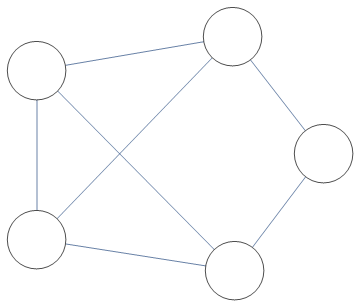
\includegraphics[width=0.18\textwidth]{vertex_insertion_left.png} & $\rightarrow$ & 
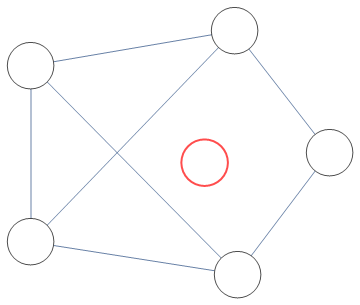
\includegraphics[width=0.18\textwidth]{vertex_insertion_right.png} & & 
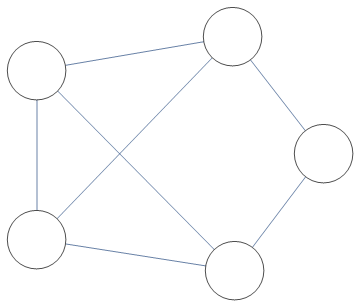
\includegraphics[width=0.18\textwidth]{edge_insertion_left.png} & $\rightarrow$ & 
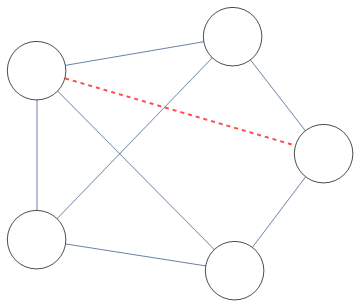
\includegraphics[width=0.18\textwidth]{edge_insertion_right.png} \\
\multicolumn{3}{c}{Node deletion} & &  \multicolumn{3}{c}{Edge deletion} \\
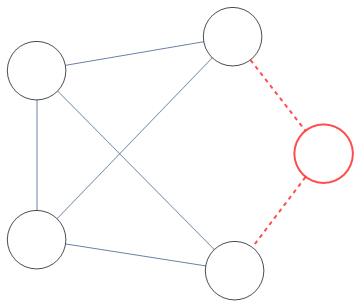
\includegraphics[width=0.18\textwidth]{vertex_deletion_left.png} & $\rightarrow$ & 
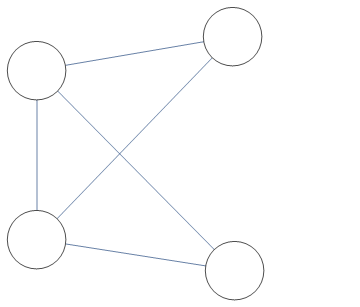
\includegraphics[width=0.18\textwidth]{vertex_deletion_right.png} & & 
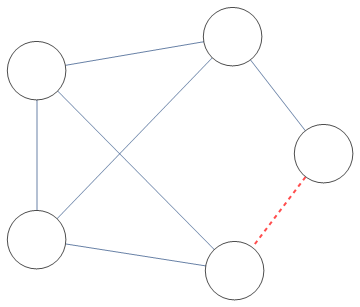
\includegraphics[width=0.18\textwidth]{edge_deletion_left.png} & $\rightarrow$ & 
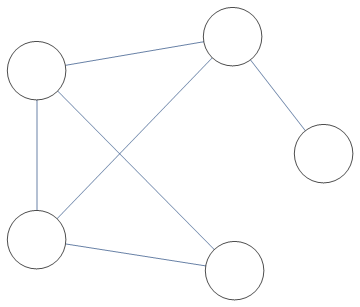
\includegraphics[width=0.18\textwidth]{edge_deletion_right.png} \\
\multicolumn{7}{c}{Node substitution} \\ & & 
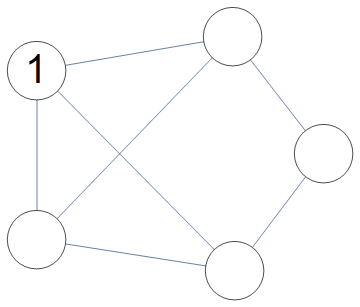
\includegraphics[width=0.18\textwidth]{vertex_substitution_left.png} & $\rightarrow$ &
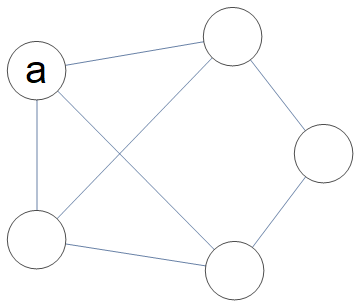
\includegraphics[width=0.18\textwidth]{vertex_substitution_right.png} & & \\
\end{tabular}
\caption{Edit operations for graphs.}
\label{fig:graph_edit_operations}
\end{figure}

For graphs, the relevant edit operations are node substitution\index{graph edit operations}, node insertion, node deletion, edge insertion, and edge deletion, as illustrated in Figure \ref{fig:graph_edit_operations}. Instead of simply taking the length of the edit path, however, we associate each of these operations with some nonnegative cost function $c(u,v)\in \R^+$ (the ``penalty" mentioned in Section \ref{section:exact_and_inexact_matching}) which avoids rewarding unnecessary edit operations by satisfying the inequality $c(u,w)\leq c(u,v)+c(v,w)$, where $u, v$, and $w$ are nodes or edges, or sometimes null nodes/edges in the case of insertion and deletion. We also assume that the cost of deleting a node with edges is equivalent to that of first deleting each of its edges and then deleting the resultant neighborless node. 

%If two graphs are isomorphic to one another, the edit distance between them is the total cost of relabeling--i.e. substituting--all $n$ nodes.

The edit distance is then the total cost of all operations involved in an edit path, and it critically depends on the costs of the underlying edit operations \cite{Bunke_1998}. This can be helpful in some cases, as it allows us to easily tweak parameters in our notion of similarity, but it is also sometimes desirable to avoid this dependence on the cost function. This is one motivation for the formulation of inexact graph matching as a continuous optimization problem, which we discuss in the next section.

Finally, we note that it was shown by Bunke in 1999 that the graph isomorphism, subgraph isomorphism, and maximum common subgraph problems are all special cases of the problem of calculating the graph edit distance under certain cost functions \cite{Bunke_1999}. 








\section{Suboptimal methods for inexact matching}

We noted previously that optimal methods for inexact graph matching tend to be very expensive and therefore only suitable for graphs of small size. To address this issue, Riesen and Bunke in 2009 introduced an algorithm for approximating the graph edit distance in a substantially faster way \cite{Riesen_2009}, which Serratosa published an improved variant of in 2014 \cite{Serratosa_2014}. This is not the only suboptimal inexact matching method in existence with the goal of suboptimally calculating a graph edit distance, but it provides an interesting connection between the seemingly disparate strategies of search space pruning and of casting the problem as one of continuous optimization.

\subsection{The assignment problem}

The key to this connection is the idea of the assignment problem. Instead of searching the space of possible edit paths to find the graph edit distance, we approximate the graph edit distance with a solution to a certain matrix optimization problem. The following definition is due to Riesen and Bunke \cite{Riesen_2009}:

\begin{definition}
Consider two sets $A$ and $B$, each of cardinality $n$, together with an $n\times n$ cost matrix $C$ of real numbers where the matrix elements $c_{i,j}$ correspond to the cost of assigning the $i$-th element of $A$ to the $j$-th element of $B$. The \textbf{assignment problem}\index{assignment problem} is that of finding a permutation $p=\{p_1,\dots,p_n\}$ of the integers $\{1,2,\dots,n\}$ which minimizes the sum $\sum_{i=1}^n c_{i,p_i}$ of the individual assignment costs.
\end{definition}

A brute force algorithm for the assignment problem would require a $O(n!)$ time complexity, which is impractical. Instead, we can use the \textbf{Hungarian method}\index{Hungarian algorithm}\index{Munkres' algorithm}. This algorithm is originally due to Kuhn in 1955 \cite{Kuhn_1955} and solves the problem in maximum time $O(n^3)$ by transforming the original cost matrix into an equivalent matrix with $n$ independent zero elements\footnote{Independent meaning that they are in distinct rows and columns.} which correspond to the optimal assignment pairs. The version of the algorithm described in \cite{Riesen_2009} is a refinement of the original Hungarian algorithm published by Munkres in 1957 \cite{munkres1957algorithms}.

\subsubsection{Relationship to the bipartite graph matching problem}

\begin{figure}[!t]
\centering
\begin{tabular}{m{0.3\textwidth}m{0.05\textwidth}m{0.3\textwidth}}
$C = $\bordermatrix{ & 1 & 2 & 3 \cr
a & 3 & 2 & 1 \cr
b & 1 & 3 & 4 \cr
c & 2 & 5 & 2 }
 & $\Leftrightarrow$ &
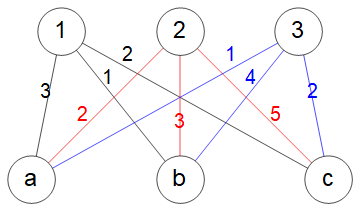
\includegraphics[width=0.3\textwidth]{bipartite_assignment_problem.png} \\
\multicolumn{3}{c}{$A = \{a,b,c\},  B=\{1,2,3\}$}
\end{tabular}
\caption{Reformulating the assignment problem as that of finding an optimal matching in a bipartite graph. The edges and their weight labels in the bipartite graph are colored to make it easier to see which weights belong to which edges.}
\label{fig:bipartite_reformulation}
\end{figure}

As noted in Section \ref{section:defining_graph_matching}, we sometimes must address the question of finding a matching \textit{in} a graph\index{matching in a graph}. This is defined as a set of edges without common nodes. It is straightforward to reformulate the assignment problem as one of finding an optimal matching within a \textbf{bipartite graph}\index{bipartite graph}, that is, a graph whose nodes can be divided into two disjoint independent sets such that no edges run between nodes of the same type. If $A$ and $B$ are two sets of cardinality $n$ as in the assignment problem, the elements of $A$ form one node group, the elements of $B$ form the other, and we define the edge weight between the $i$-th element of $A$ and the $j$-th element of $B$ to be the cost of that assignment, as shown in Figure \ref{fig:bipartite_reformulation}. The assignment problem is therefore also referred to as the bipartite graph matching problem.

\subsubsection{Relationship to graph edit distance}

To connect the assignment problem to graph edit distance computation, we define a cost matrix $C$ such that each $c_{i,j}$ entry corresponds to the cost of substituting the $i$-th node in our source graph to the $j$-th node in our target graph \cite{Riesen_2009}. We can generalize this approach further to handle graphs with different numbers of nodes by using a modified version of the Hungarian method which applies to rectangular matrices \cite{bourgeois1971extension} by considering node insertions and deletions as well as substitutions. 

In this modified version of the Hungarian method, the resulting cost matrix (again, definition due to Riesen and Bunke \cite{Riesen_2009}) becomes 

\[
C = \left[
\begin{array}{cccc|cccc}
c_{1,1} & c_{1,2} & \dots & c_{1,m}     &     c_{1,-} & \infty & \dots & \infty \\
c_{2,1} & c_{2,2} & \dots & c_{2,m}     &     \infty & c_{2,-} & \ddots & \vdots \\
\vdots & \vdots & \ddots & \vdots          &     \vdots & \ddots & \ddots & \infty \\ 
c_{n,1} & c_{n,2} & \dots & c_{n,m}     &     \infty & \dots & \infty & c_{n,-} \\ \hline

c_{-,1} & \infty & \dots & \infty             &     0 & 0 & \dots & 0 \\ 
\infty & c_{-,2} & \ddots & \vdots          &     0 & 0 & \ddots & \vdots \\ 
\vdots & \ddots & \ddots & \infty           &     \vdots & \ddots & \ddots & 0\\ 
\infty & \dots & \infty & c_{-,m}            &    0 & \dots & 0 & 0 \\ 
\end{array}
\right],
\]
where $n$ is the number of nodes in the source graph, $m$ is the number of nodes in the target, and a $-$ is used to represent null values. The upper left corner of this matrix represents the cost of node substitutions, and the bottom left and top right corners represent the costs of node insertions and deletions. Since each node can be inserted or deleted at most once, the off-diagonal elements of these are set to infinity. Finally, since substitutions of null values should not impose any costs, the bottom right corner of $C$ is set to zero.

This is only a rough approximation of the true edit distance, as it does not consider any information about the costs of edge transformations. We can improve the approximation by adding the minimum sum of edge edit operation costs implied by a node substitution to that substitution's entry in the cost matrix, but we still only have a suboptimal solution for the graph edit distance problem even though the assignment problem can be solved optimally in a reasonable amount of time.

\subsubsection{Other suboptimal graph matching methods using the assignment problem}

Approximating the graph edit distance is far from the only graph matching strategy which is based around the assignment problem. Instead of a cost matrix based around the cost function of a graph edit distance measure, we can incorporate other measures of similarity or affinity between nodes. The advantage of this approach is that we can incorporate both topological\footnote{That is, information derived directly from the structure of a network.} and external notions of similarity into our definition. To be effective, this strategy requires a relevant source of external information, and as a result is much more prevalent in biological applications. In either case, we attempt to maximize the edges in the induced common subgraph only indirectly; a good cost function will be an effective proxy for how much a certain node pairing will contribute to a good overall mapping, but it does not directly maximize the edge preservation.

\subsection{Weighted graph matching vs. the assignment problem}

Most of the suboptimal graph matching methods we observed are based around either the assignment problem or around some formulation of the weighted graph matching problem. The \textbf{weighted graph matching problem}\index{weighted graph matching problem} is typically defined as finding an optimum permutation matrix which minimizes a distance measure between two weighted graphs; generally, if $A_G$ and $A_H$ are the adjacency matrices of these, both $n\times n$, we seek to minimize $||A_G - PA_HP^T||$ with respect to some norm \cite{Umeyama_1988, Koutra_2013, Almohamad_1993} or to minimize some similarly formulated energy function \cite{Gold_1996}. The specific definition depends on the technique being used to solve the optimization problem.

Weighted graph matching is an inexact graph matching method, and its techniques are generally suboptimal, searching for a local minimum of the corresponding continuous optimization problem. There is a wide variety of techniques in use, including linear programming \cite{Almohamad_1993}, eigendecomposition \cite{Umeyama_1988}, gradient descent \cite{Koutra_2013}, and graduated assignment \cite{Gold_1996}. Other techniques mentioned in \cite{Almohamad_1993, Umeyama_1988, Gold_1996, Conte_2004} include Lagrangian relaxation, symmetric polynomial transformation, replicator equations, spectral methods other than eigendecomposition, neural networks, and genetic algorithms.

The weighted graph matching problem is similar to the assignment problem in that we seek a permutation between the $n$ nodes of two graphs, but unlike the assignment problem, there is no need to define a cost or similarity matrix ahead of time. Instead, we directly measure the quality of a permutation assignment with respect to the structure of a graph and optimize this quantity to find our matching. This allows us to avoid relying on the heuristics inherent in any formulation of a cost or similarity matrix, but it also means we cannot easily incorporate external information into our solution of the problem. We also cannot choose to favor alignments with desirable properties other than conserved edges; for example, we may prefer a connected alignment to a more scattered one, even if it conserves fewer edges. Whether weighted graph matching techniques are preferable to assignment problem-based strategies is therefore dependent on the specific problem to be solved. 









%%%%%%%%%%%%%%%%%%%%%%%%%%%%%%%% CHAPTER 5 %%%%%%%%%%%%%%%%%%%%%%%%%%%%%%%%%%%%%%%







\chapter{Biology}\label{chapter:systems_biology}

\section{Motivation}

A fundamental goal in biology is to understand complex systems in terms of their interacting components. Network representations of these systems are particularly helpful at the cellular and molecular level, at which we have large-scale, experimentally determined data about the interactions between proteins, genes, and metabolites. In the past twenty years, there has been an explosion of availability of interaction data between biomolecules, paralleling the surge of DNA sequence information availability that was facilitated by the Human Genome Project \cite{humanGenomeProject}. Sequence information comparison tools have been revolutionary in advancing our understanding of basic biological processes, including our models of evolutionary processes and disease \cite{HGPimpact}, and the comparative analysis of biological networks presents a similarly powerful method for organizing large-scale interaction data into models of cellular signaling and regulatory machinery \cite{Sharan_2005}. 

In particular, we can use network comparison to address fundamental biological questions such as ``Which proteins, protein interactions, and groups of interactions are likely to have equivalent functions across species?", ``Can we predict new functional information about proteins and interactions that are poorly characterized, based on similarities in their interaction networks?", and ``What do these relationships tell us about the evolution of proteins, networks, and whole species?" \cite{Sharan_2006}. Comparison strategies and metrics are also key to developing mathematical models of biological networks which represent their structure in a meaningful way--a key step towards understanding them. For example, good comparison techniques allow us to model dynamical systems on biological networks \cite{Watts_1998} (e.g., the spread of infectious diseases) and to create appropriate null hypotheses for drawing conclusions about experimental networks\footnote{Section 2.3.1 in \cite{Hayes_2013} is a brief and superb discussion of the importance of modeling biological networks.}  \cite{Hayes_2013}.

\section{Comparison to pattern recognition}

As mentioned in Chapter \ref{chapter:pattern_recognition}, we observed two overwhelmingly dominant network comparison strategies in biology applications. We  use the term \textit{comparison} strategies and not \textit{matching} or \textit{alignment} strategies because unlike pattern recognition, not all biological applications seek a mapping between two networks. This is a result of the difference between the typical networks with which each field is concerned.

In pattern recognition, graphs are primarily a convenient data structure to represent the objects that we would like to compare and do not necessarily represent inherent real-world relationships. The goal of comparison is typically to find the closest object from a large database, and seeking an ``isomorphism with tolerance" is a viable strategy, as we typically have a small number of vertices and expect to be able to find a close structural match.  

By contrast, in biology we work with networks which are very large, typically incompletely explored, non-deterministic\footnote{Since biological networks are constructed entirely based on experimental data, edges can only ever represent probabilities, and their analysis must take this into consideration.}, and which we cannot expect to be ``almost the same" globally. Furthermore, we have highly significant external information about their vertices, such as BLAST scores (sequence similarities)\index{BLAST scores} or known functions of individual proteins, and every edge and subgraph corresponds to real-world interactions that have real-world meaning. Mapping-seeking comparison strategies for biology do not seek to give an overall measure of the similarity between two graphs, but to find regions which are conserved between two or more networks, under what Flannick et al.\ \cite{flannick2006graemlin} calls ``perhaps the most important premise of modern biology": the assumption that evolutionary conservation implies functional significance.

When comparing and analyzing biological networks as a whole, we can find meaning using strategies other than seeking a mapping between networks. These are generally based on investigating the frequencies and/or distributions of relevant subgraphs of a large network, i.e., graphlets and motifs, which we now introduce by way of generalization of the network statistics discussed in Chapters 1 and 2.

%\begin{table}[h]
%\centering
%\begin{tabular}[t]{L{0.3\linewidth}L{0.3\linewidth}L{0.3\linewidth}}
%\textbf{Graph matching for pattern recognition} & \textbf{Biological network alignment} & \textbf{Alignment-free biological network comparison} \\ \hline\hline \noalign{\medskip}
%Seeks to recognize objects based on their graph representations & Seeks to find conserved regions between multiple networks & Seeks to compare networks on a global scale \\\noalign{\medskip}
%Attempts to find a mapping or near-mapping between graphs & Attempts to find a mapping or near-mapping between networks & Does not attempt to find a mapping \\\noalign{\medskip}
%Deals with large numbers of small graphs & Deals with small numbers of large or very large networks & Deals with a variable number of large or very large networks \\\noalign{\medskip}
%Expects to find graphs which are near-isomorphic & Networks are not generally near-isomorphic & Networks are not generally near-isomorphic \\\noalign{\medskip}
%Graphs are simply a convenient data structure to represent objects we would like to compare & Each vertex and edge independently represents meaningful information about the real world & Each vertex and edge independently represents meaningful information about the real world\\
%\end{tabular}
%\caption{Summary of differences between graph matching for pattern recognition and biological network comparison. Note: I'm unsure whether this table is worth including.}
%\label{tab:bio_vs_CS_summary}
%\end{table}
%







\section{Network statistics and measures}


In Table \ref{tab:network_table}, we compared various network statistics for our constructed citation network and its pruned version to two other citation networks and two other random networks. Our goal in doing so was to determine whether the calculated statistics were noteworthy in some way. Without some kind of context, we cannot tell, for example, whether a diameter of ten is above average, remarkably small, or somewhere in between, or if it is typical to have 96\% of the vertices in the network contained in the giant component. 

\begin{figure}[t]
\renewcommand{\arraystretch}{1.5}
%\fbox{\begin{minipage}{\textwidth}
\centering
\hfill
\begin{tabular}[c]{ccccl}
\multicolumn{5}{l}{\underline{\textbf{Network comparison with univariate measures}}} \\ \noalign{\smallskip}
Network & $\rightarrow$ & Something in $\R^n$ & \multirow{2}{0.06\linewidth}{$\Big\rangle\rightarrow$} & \multirow{2}{0.37\linewidth}{Similarity score derived from some aggregation measure on $\R^n$} \\ \noalign{\smallskip}
Network & $\rightarrow$ & Something in $\R^n$  \\ \noalign{\medskip}
\textbf{Examples:} & \multicolumn{4}{p{0.7\textwidth}}{Any metric on $\R^n$ applied to number of vertices and edges, mean degree, diameter, connectivity, degree or centrality distributions, local graphlet counts, graphlet degree distributions, etc.} \\
\end{tabular}
\hfill
\vspace{0.5cm}
\begin{tabular}[c]{cclcc}
\multicolumn{5}{l}{\underline{\textbf{Network comparison with bivariate measures}}} \\ \noalign{\smallskip}
Network &  \multirow{2}{0.05\linewidth}{$\Big\rangle\rightarrow$} & \multirow{2}{0.19\linewidth}{Mapping process} & \multirow{2}{0.05\linewidth}{$\rightarrow$} \multirow{2}{0.32\linewidth}{Similarity measure derived from the mapping}\\ \noalign{\smallskip}
Network & \\ \noalign{\medskip}
\textbf{Examples:} & \multicolumn{4}{p{0.72\textwidth}}{Graph edit distance; node correctness, edge correctness, induced conserved structure \cite{Patro_2012}, or symmetric substructure score \cite{Saraph_2014} with respect to an alignment; MCS-related metrics (i.e., \cite{Bunke_1998})} \\
\end{tabular}
\caption{A summary of the distinction between univariate and bivariate measures.}
\label{fig:univariate_and_bivariate}
%\end{minipage}}

\end{figure}

That is, we know that our network statistics are only meaningful when we compare them to the same statistics for other networks. 
Network statistics such as vertex count, edge count, and diameter can therefore be thought of as a similarity measure between two networks\footnote{See \cite{Aittokallio_2006} for a discussion of how these are relevant to biology specifically.}. This is generally a much weaker form of similarity than even suboptimal inexact graph matching, but the more important distinction is that these are \textbf{univariate}\index{univariate measure} measures. That is, they map from a single network to $\R^n$, in contrast to \textbf{bivariate}\index{bivariate measure} measures, which give us a single number representing the similarity between two networks. The distinction between univariate and bivariate measures is illustrated in Figure \ref{fig:univariate_and_bivariate}. We can treat univariate measures as bivariate by using some sort of metric or other aggregation measure on their output for two different networks, but they have the additional advantage of allowing us to classify networks based on their output, rank them on a spectrum, and so on. This is particularly important for creating random models of networks that share the key properties of the real-world networks we would like to study \cite{Hayes_2013, Watts_1998}.

\subsection{Local and global network statistics}

Network statistics like vertex and edge count, diameter, size of giant component, and assortativity values are all \textbf{global}\index{global network statistics}, meaning they give us a single value for the entire graph. The centrality measures we introduced in Section \ref{section:centrality}, in contrast, are \textbf{local}\index{local network statistics}, meaning they give us a value at each vertex. Examples of global and local network statistics can be found in Table \ref{tab:local_vs_global_statistics}. So far, we have seen these values used to rank vertices and choose a small number of them for further analysis, but we can gain insight into the graph as a whole by looking at distributions of these values.

The \textbf{degree distribution}\index{degree distribution} is the simplest example of this. We count the number of vertices with degree zero, one, two, and so on, and display the results in a histogram. For a directed graph, we have distributions for both indegree and outdegree. Further information about degree distributions and their relevance can be found in \cite{newman2010}.

\begin{table}[!t]
\renewcommand{\arraystretch}{1.5}
\centering
\begin{tabular}{L{0.13\linewidth}L{0.25\linewidth}L{0.45\linewidth}}
\hline
\textbf{Type} & \textbf{Description} & \textbf{Examples} \\ \hline
Global & Single value for an entire network & Mean degree, maximum degree, diameter, edge density, assortativity, global clustering coefficient \\ 
Local & Value at each vertex in a network & Indegree, outdegree, graphlet degrees, betweenness centrality, closeness centrality, HITS centralities, local clustering coefficient  \\
\hline
\end{tabular}
\caption{A summary of the distinction between local and global network statistics.}
\label{tab:local_vs_global_statistics}
\end{table}









\section{Graphlets and motifs}

\textbf{Graphlets}\index{graphlets} are small connected non-isomorphic induced subgraphs of a simple undirected network \cite{Przulj_2007}, introduced by Nata\u{s}a Pr\u{z}ulj in the mid-2000s for the purpose of designing a new measure of local structural similarity between two networks based on their relative frequency distributions.

\begin{figure}[t]
\centering
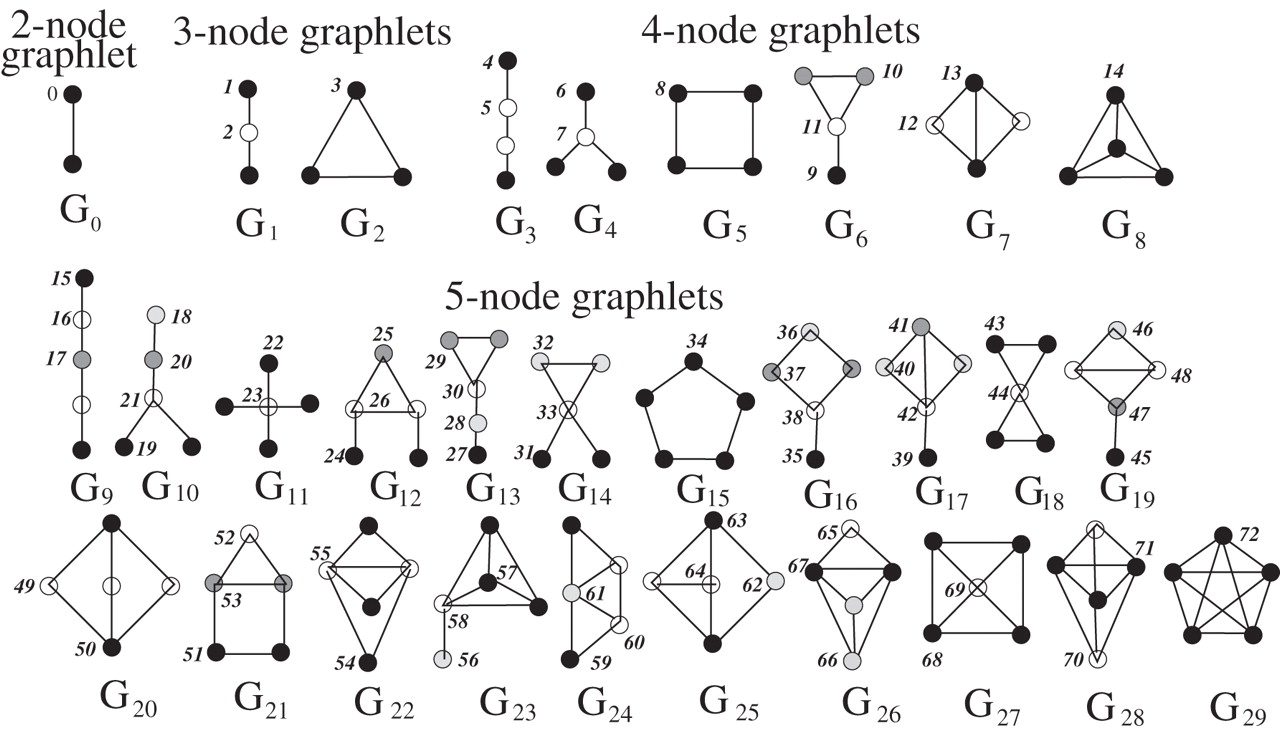
\includegraphics[width=\textwidth]{graphlets_figure.png}
\caption{The 73 automorphism orbits for the 30 possible graphlets with 2-5 nodes. In each graphlet, vertices belonging to the same automorphism orbit are the same shade. Figure reproduced from \cite{Przulj_2007}.}
\label{fig:graphlets}
\end{figure}

First, we recall that the degree distribution measures, for each value of $k$, the number of vertices of degree $k$. In other words, for each value of $k$, it gives the number of vertices touching $k$ edges. We note that a single edge is the only graphlet with two nodes and call it $G_0$. The degree distribution can therefore be thought of as measuring how many vertices touch one $G_0$ graphlet, how many vertices touch two $G_0$ graphlets, and so on.

We can generalize this idea to larger graphlets and count how many vertices touch a certain number of each graphlet $G_0, \dots, G_{29}$, where $G_0,\dots, G_{29}$ are defined as in Figure \ref{fig:graphlets}. For example, the $G_2$ distribution measures how many vertices touch one triangle, two triangles, and so on. However, we notice that for most graphlets larger than two vertices, \textit{which} vertex of the graphlet we touch is topologically relevant; for example, touching the middle node of $G_1$ is different from touching an end node. This is because the end and middle vertices are in different \textbf{automorphism orbits}\index{automorphism orbits}. Two vertices are in the same automorphism orbit if they can be mapped to each other in an automorphism (i.e., an isomorphism from the graph to itself). Intuitively, this means that we have no way of telling them apart without labeling the graph. If two vertices are in different automorphism orbits, we can tell them apart using their degree, the neighbors of their neighbors, and so on, as we did in our demonstration of the Ullmann subgraph isomorphism algorithm.

The \textbf{graphlet degree}\index{graphlet degree} therefore measures how many of a certain graphlet \textit{in a specific automorphism orbit} each vertex touches. There are 73 different automorphism orbits for the thirty graphlets with 2-5 nodes, and we therefore obtain 73 \textbf{graphlet degree distributions (GDDs)}\index{graphlet degree distribution} analagous to (and including) the degree distribution. Since these are based on the neighborhoods of each vertex, they measure the local structure of a graph. 

An example of the $G_0$ and $G_2$ distributions for the protein-protein interaction (PPI) networks of \textit{Mycoplasma genitalium} (an STD) and \textit{Schizosaccharomyces pombe} (yeast) is shown in Figure \ref{fig:GDD_demo}, with corresponding statistics in Table \ref{tab:ppi_networks}. We obtained both networks from the STRING database \cite{szklarczyk2014string} and included links with an interaction confidence score above 950, i.e., those representing 95\% probability of an interaction between two proteins. 

\begin{table}[t]
\centering
{\setlength\extrarowheight{3pt}\setstretch{1}\fontsize{11}{13}\selectfont
\begin{tabular}{L{0.31\linewidth}C{0.085\linewidth}C{0.08\linewidth}C{0.11\linewidth}C{0.11\linewidth}C{0.11\linewidth}}
\hline
 & Vertices & Edges & Clustering & Maximum $G_0$ degree & Maximum $G_2$ degree \\ \hline

\textit{Mycoplasma genitalium} & 444 & 1860 &  0.758 & 66 & 1376 \\ 
Random (match degree seq.) & 444 & 1860 & 0.420 & 66 & 774  \\ 
Random (match size) & 444 & 1860 &  0.022 & 17 & 6 \\ \hline
\textit{Schizosaccharomyces pombe} & 5100 & 30118 & 0.757 & 213 & 14592 \\ 
Random (match degree seq.) & 5100 & 30118 &  0.150 & 213 & 3606 \\ 
Random (match size) & 5100 & 30118 & 0.002 & 26 & 3 \\ \hline
\end{tabular}
}
\caption{Statistics for PPI networks of two small organisms and two comparable random graphs for each. The ``clustering" value is the global clustering coefficient\index{global clustering coefficient} \cite{newman2010}, which measures the fraction of connected triplets in the network which are closed.}
\label{tab:ppi_networks}
\end{table}

\begin{figure}[!ph]
\centering
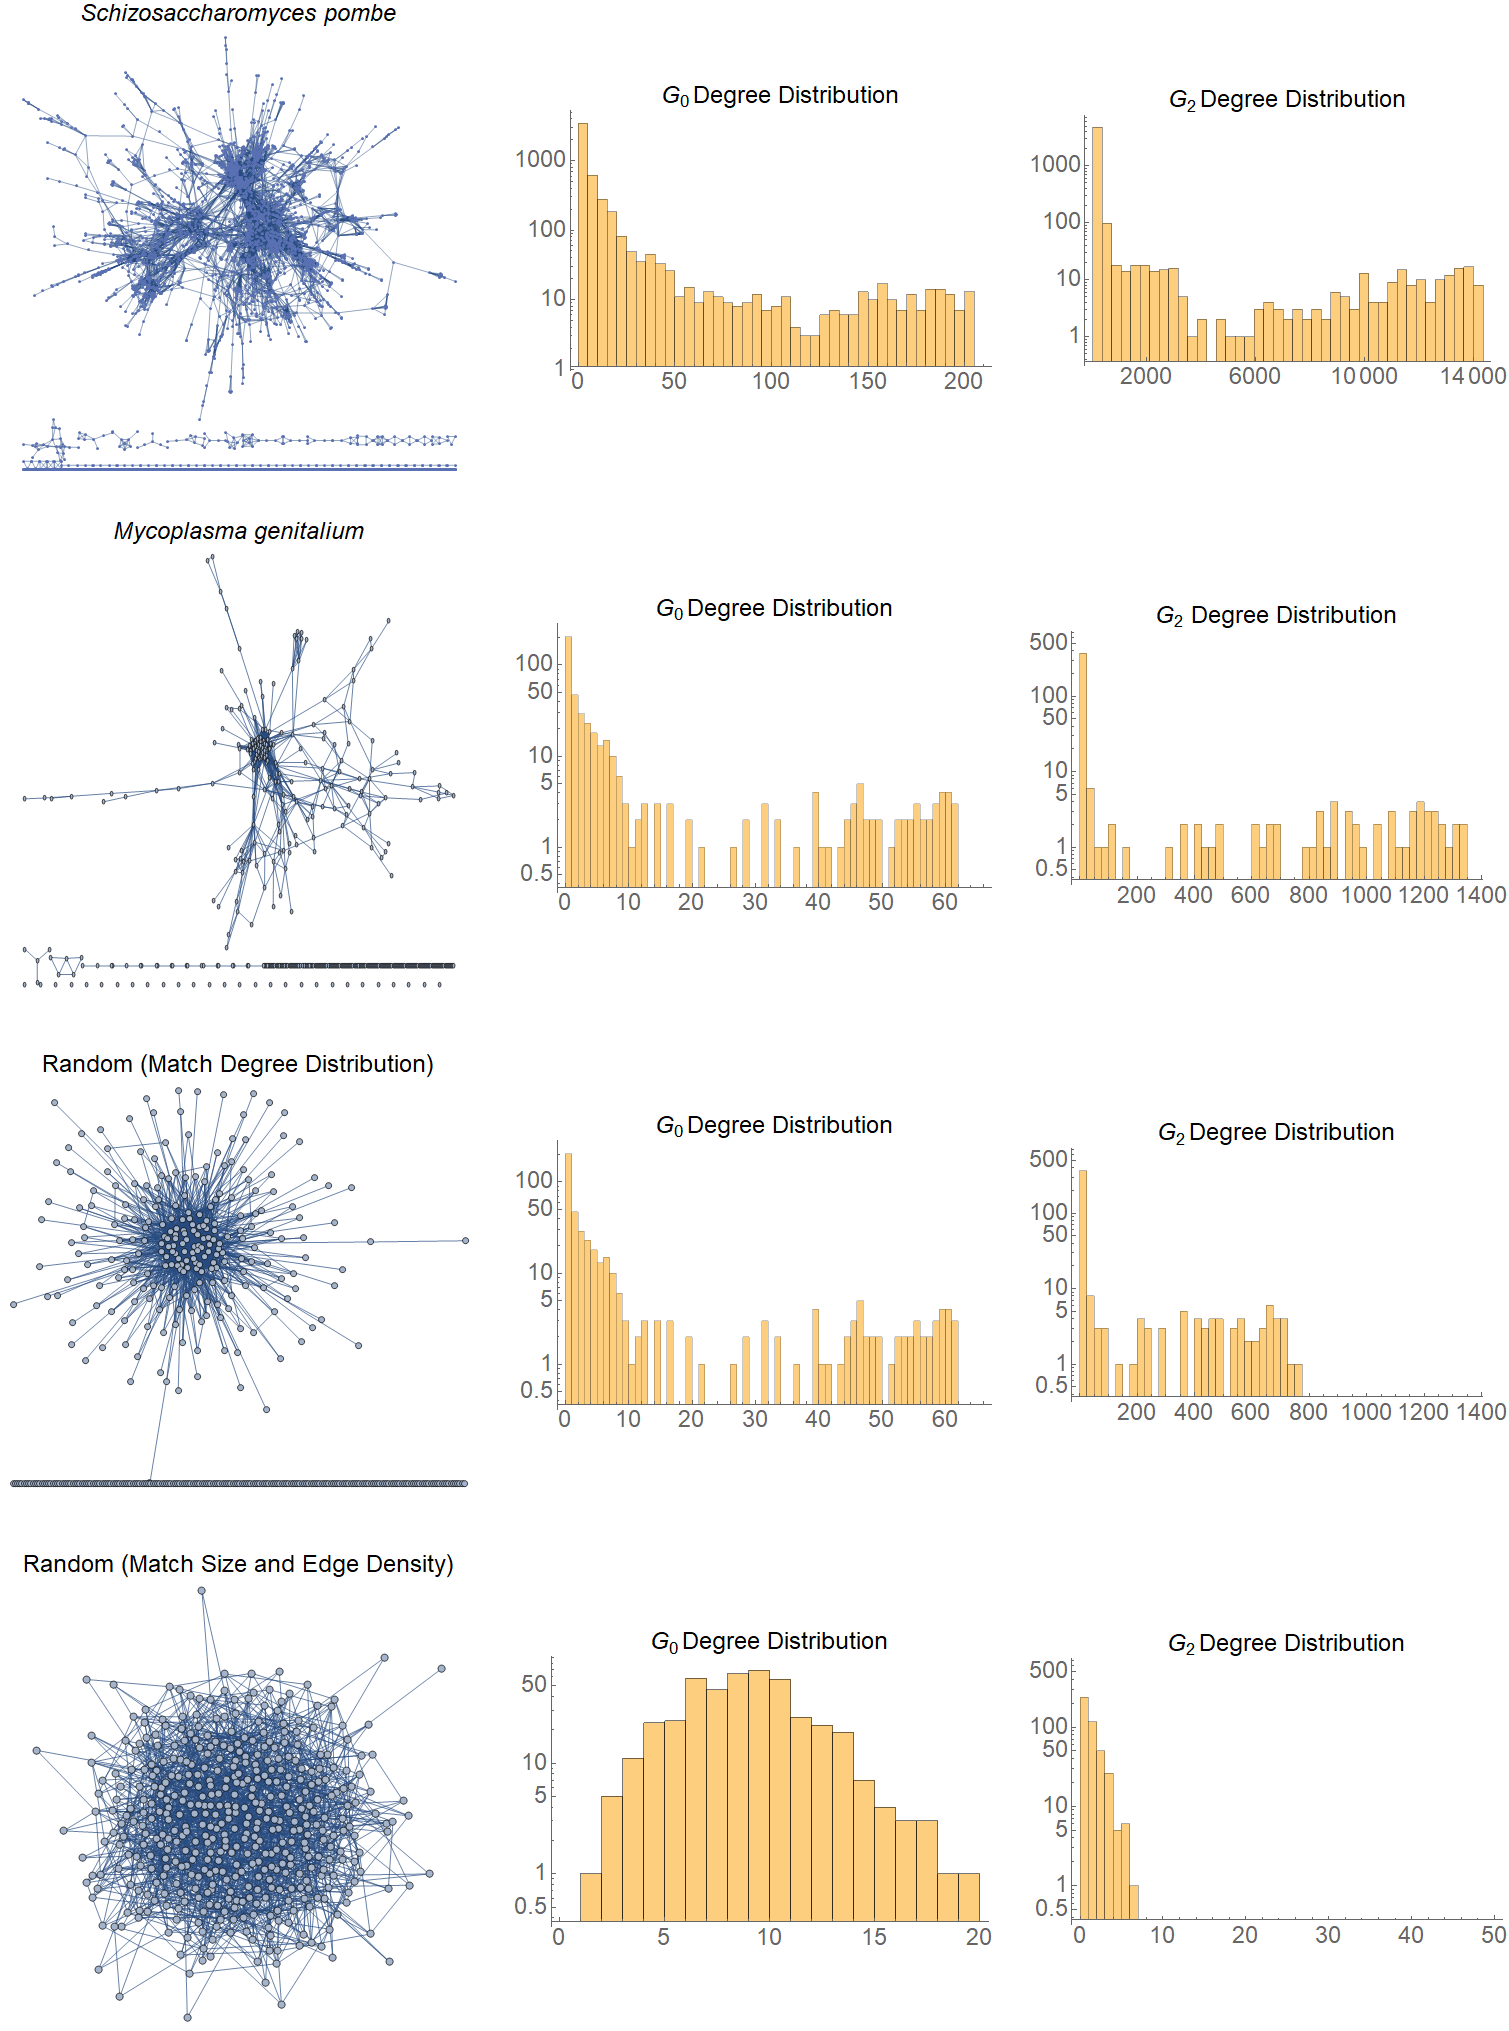
\includegraphics[width=0.95\textwidth]{graphlet_degree_distributions.png}
\caption{Visualizations and $G_0$ and $G_2$ distributions for the PPI networks of \textit{S. pombe}, \textit{Mycoplasma genitalium}, and two randomly generated networks comparable to the latter.}
\label{fig:GDD_demo}
\end{figure}

When we look at the maximum $G_2$ degree, we can easily distinguish between a real network and a random network with the same degree sequence; we can also see different patterns in the shape of the $G_2$ distributions for the PPI networks of our two model organisms. We can guess that the varying shapes of all 73 GDDs would help us distinguish between different graphs in a meaningful way. In order to use these distributions for computational network comparison, however, we must somehow reduce this large quantity of information to a single measure. Pr\u{z}ulj introduces one possible method in \cite{Przulj_2007} by considering the Euclidean distance between each GDD for two networks, after appropriate scaling and normalization, and then taking the arithmetic or geometric mean over this distance for all 73 graphlet automorphism orbits. Other methods are of course possible and potentially better, depending on the application in question.

\subsection{Graphlets vs. Motifs}

Network \textbf{motifs}\index{motif} are similar to graphlets in that they are both small induced subgraphs of large networks. Unlike graphlets, however, the definition of motifs requires these subgraphs to be \textit{statistically overrepresented} in the network \cite{Milo_2002}; that is, they are patterns of interactions which occur more frequently than you would reasonably expect due to random chance. In a random graph with the same degree sequence(s) as a real network, we are not likely to see connected triangles, for example--but as we can see in Table \ref{tab:ppi_networks} and Figure \ref{fig:GDD_demo}, connected triangles appear frequently in real biological networks, associated with feedback or feed-forward loops in transcription and neural networks, clusters in protein interaction networks, and so on \cite{Berg_2004}. We can generalize further to seek \textbf{topological motifs}, which are statistically overrepresented ``similar" network sub-patterns. 

Such patterns can be used as a first step towards understanding the basic structural elements particular to certain classes of networks \cite{Milo_2002}; different types of networks contain different types of elementary structures which reflect the underlying processes that generated them, and as discussed in \cite{Berg_2004}, motifs are in fact indicative of biological functions. These methods are a useful way to distinguish patterns of biological function in the topology of molecular interaction networks from random background, but they are not well-suited for full-scale comparison of multiple networks \cite{Przulj_2007}. They are sensitive to the choice of random network model used to determine statistical significance, and they ignore subgraphs with low or average frequency. These low-frequency subgraphs may still be functionally important, especially if such subgraphs are consistently seen across multiple real networks despite occurring rarely within any individual one. Graphlets are one way to address this issue; alignment strategies are another. We also note that \cite{Przulj_2007} defines graphlets for undirected graphs only, while the motifs discussed in \cite{Milo_2002} and \cite{Berg_2004} are primarily directed. In both cases, however, the definition does not include multiedges or self-loops.


\subsubsection{Computational complexity}

We already know that subgraph isomorphism is a computationally expensive problem. Exhaustively finding all occurrences of small isomorphic or near-isomorphic subgraphs in a network is infeasible for the gene and PPI networks of all but small organisms such as \textit{E. coli} \cite{Emmert_Streib_2016}. As a result, motif search in large networks (which requires an exhaustive search over an entire ensemble of random graphs in order to determine statistical significance) is generally limited to subgraphs of at most five nodes. Graphlet statistics are similarly expensive to compute. In order to process the interaction networks of higher organisms, search heuristics and estimation procedures must be used.

\subsection{Netdis}

Netdis \cite{Ali_2014}, introduced by Ali et al.\ in 2014, is another method for network comparison which is primarily based on counting the occurrences of small subgraphs in a larger network. For each vertex, we count the number of occurrences of each possible graphlet of 3-5 nodes in a neighborhood of radius two around it. Each vertex is thereby associated with a vector of graphlet counts, which is normalized with respect to the same counts for a gold standard PPI network, as a proxy for the counts we would expect to see in a suitable random model for a typical PPI network. These centered counts are then combined into an overall statistic. 

This statistic is used in \cite{Ali_2014} to correctly separate random graph model types and to build the correct phylogenetic tree of species based on their protein interaction networks, showing that Netdis is a relevant comparison method for large networks. The method is also highly tractable; since we only search for subgraphs in a given neighborhood, computational complexity grows about linearly with the number of vertices in a network if neighborhood sizes stay relatively small, and Netdis is therefore well-suited for full-scale comparison of many large networks.

We note that while Netdis uses graphlet counts, it is not a generalization or special case of graphlet degrees. When counting graphlets in the two-step neighborhood of a vertex, we only need to consider the 29 possible graphlets of 3-5 nodes, rather than their 72 possible automorphism orbits.
Not all the graphlets a vertex touches will necessarily be present in its two-step neighborhood, and we can also have graphlets in the two-step neighborhood of a vertex which do not directly touch the vertex itself. 








\section{Local and global network alignment}

In graph matching applications and in subgraph counting, any mappings found by an algorithm have not been the primary result of interest in network comparison. When calculating graphlet statistics and network motifs, we do perform graph matching, but the subgraphs involved are so small that whether the matching algorithm is mapping-seeking is not a particularly relevant question; the computational difficulty is a result of the difficulty in enumerating these subgraphs, not a result of matching them to each other. In pattern recognition, we use inexact matching methods in order to allow for error in the comparison of slightly larger\footnote{Typically up to a hundred nodes at most, based on the experimental results reported by our references.} graphs that should represent the same or similar objects. There are enough nodes to make an exhaustive search difficult, so the matching method we use matters, but the mapping between two networks does not typically give us relevant real-world insights about the structures they represent.

When comparing large biological networks, however, this is not the case, and we therefore frequently seek regions of similarity and dissimilarity in two or more large networks (thousands of nodes and tens of thousands of edges). Just as longer DNA sequences which are conserved across species indicate functional significance and can help classify evolutionary relationships, larger subnetworks of biomolecular interactions which are conserved across species are likely to represent true functional modules\footnote{Throughout the rest of this work, we will use \textit{module}\index{module} to refer to a subgraph of a biological network which is larger than a motif, but still relatively small compared to a full-size network, and which is known to have functional significance.}  \cite{Sharan_2006} and give insight into evolutionary processes \cite{Ali_2014}. To find these conserved regions, we seek an \textbf{alignment}\index{alignment}, or a mapping between vertices in two or more networks which approximates the true structure they have in common. Alignment algorithms may or may not be able to find an isomorphism, if one exists, but this is not important when the networks being aligned are essentially guaranteed to not be isomorphic anyway.

\subsection{Local vs. global alignment}

\renewcommand{\topfraction}{0.65}
\begin{figure}[!t]
\centering
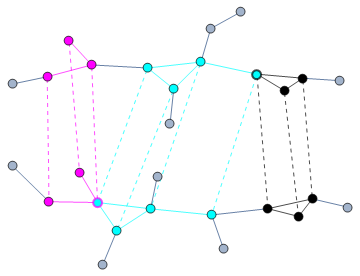
\includegraphics[width=0.5\textwidth]{local_alignment.png}
\vspace{5pt}
\caption{Local alignment of a network. Vertices may be used for multiple ``pieces" of the overall mapping, i.e., the mapping is not required to be one-to-one.}
\label{fig:local_alignment}
\vspace{15pt}
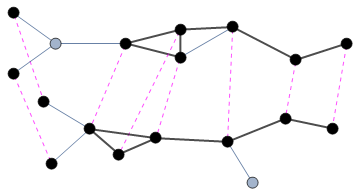
\includegraphics[width=0.5\textwidth]{global_alignment.png}
\vspace{5pt}
\caption{Global alignment of a network. Not all vertices must be mapped to a vertex in the other network, but the mapping must be one-to-one in both directions when they are.}
\label{fig:global_alignment}
\end{figure}

Alignment strategies for biological applications fall into two categories: local alignment, and global alignment. In both cases, we seek to find regions of similarity between networks, and mappings do not need to be defined for every vertex in each network. 

In \textbf{local alignment}\index{local alignment}, the goal is to find local regions of isomorphism between the two networks, where each region implies a mapping which is independent of the others. These mappings do not need to be mutually consistent; that is, a vertex can be mapped differently under different regions of the mapping, as illustrated in Figure \ref{fig:local_alignment}. We can choose a locally optimal mapping for each region of similarity, even if this results in overlap. In \textbf{global alignment}\index{global alignment}, by contrast, we must define a single mapping across all parts of the input, even if it is locally suboptimal in some regions of the networks \cite{Singh_2007}. 

To understand the distinctions between these two alignment strategies, we must understand the motivations behind their development, and the biological implications of their results\footnote{The first few paragraphs of \cite{flannick2006graemlin} are a concise and effective overview of the origins and goals of biological network alignment and its relationship to sequence alignment.}. The study of biological \textit{networks} has been guided first and foremost by the study of biological \textit{sequences}, primarily DNA sequences, and the development of biological network alignment closely parallels that of sequence alignment\index{sequence alignment}\footnote{A timeline comparing these developments as of 2006 can be found in \cite{Sharan_2006}.}. 
\newpage
{\flushleft Sequence alignment is based on the assumptions that:}

\begin{enumerate}
\item Patterns which occur frequently (motifs) are likely to have functional significance. 
\item Sequence regions which are conserved across multiple species are likely to have

 functional significance.
\item The degree to which sequences differ is related to their evolutionary distance.
\end{enumerate}

The study of (i) is roughly the domain of local sequence alignment, while the study of (ii) and (iii) is roughly the domain of global sequence alignment. Local network alignment, by analogy, searches for highly similar network regions that likely represent conserved functional structures (i.e., evolutionarily conserved building blocks of cellular machinery), which often results in relatively small mapped subnetworks and in some network regions not being a part of the alignment. Global network alignment, on the other hand, looks for the best superimposition of the entire input networks  (i.e., a single comprehensive mapping between the sets of protein interactions from different species), which typically results in large but suboptimally conserved mapped subnetworks \cite{guzzi2017survey}.

Sequence alignment cannot be perfectly generalized to network alignment; sequence complexity is linear, while network complexity is combinatorial. An alignment of two sequences of length $m$ and $n$ can be done in $O(mn)$ time using the Needleman-Wunsch algorithm \cite{Wunsch_time_is_over}\index{Needleman-Wunsch algorithm}, but the closest analogue of sequence alignment for networks is the maximum common induced subgraph problem, which we know to be NP-hard (see Table \ref{NP_classifications}). As a result, the analogy to sequence alignment must be compromised for the sake of tractability.

This is least necessary in the case of very small subgraphs; searching exhaustively for very small subgraphs in a network is computationally expensive, but tractable. As a result, network motifs are a fairly straightforward generalization of the idea of sequence motifs\footnote{Graphlets can be thought of as a generalization of motifs; instead of counting all occurrences of a pattern and asking whether that number is abnormally high, we look at the \textit{distribution} of all occurrences of a small pattern, and take it as it is.}.

For slightly larger subgraphs, a common compromise is to search for a predetermined pattern, rather than for \textit{all} frequently occurring patterns. The number of possible patterns on 2-5 vertices is small enough to make searching for all of them feasible, as in graphlets and motifs, but we can also search a less well-known network or the network of another species for a certain pathway or module already known to be significant. Another compromise is to construct an alignment based on a deterministic notion of which nodes are similar and which edges are conserved; since we have significant amounts of external information about the vertices (sequence similarity of proteins, etc.), this can yield useful results. Not all local alignment algorithms in our references make the compromise of searching only for predetermined patterns--although this is a common strategy--but they \textit{do} all define alignments deterministically through external information; the more general definition of local alignment compared to global alignment makes it too broad a question for network topology to answer on its own.

Global alignment, on the other hand, makes the compromise of investigating the assignment problem rather than the maximum common induced subgraph problem. The assignment problem has the advantage of being fully solvable in low polynomial time via the Hungarian algorithm (and we can get good results with even cheaper methods), which allows us to handle much larger networks. The tradeoffs are that our ability to find conserved networks is highly dependent on the definition of our cost function for mapping pairs of nodes onto each other, and we introduce a need for heuristic measures of quality for the resulting assignment. The cost function is generally based on a combination of external (i.e., sequential and/or functional) and topological information about the vertices in a network. Unlike local alignment, the use of external information is frequently optional, and it is never the primary driver of the results.

At the time IsoRank\index{IsoRank} \cite{Singh_2007} was introduced in 2007, the global network alignment problem had received little attention in the literature; no papers referencing ``global alignment" or ``global network alignment" which address the topic as we have defined it were published any earlier than 2007. After IsoRank was introduced, however, global alignment began to receive significant attention, and most of the papers in our dataset which address biological network alignment address global alignment. The transition from local to global alignment seems to have occurred as biological network comparison strategies began to increasingly seek to learn from topological network structure rather than deterministically attempting to generalize sequence alignment, and as increasingly accurate PPI network data and increased computational resources for network analysis became available.

\subsection{Local alignment algorithms}

\subsubsection{PathBLAST and NetworkBLAST} The PathBLAST algorithm\index{PathBLAST} introduced by Kelley et al.\ in 2004 \cite{kelley2004pathblast, Sharan_2005, Sharan_2006} and its successor NetworkBLAST \cite{kalaev2008networkblast} both search for query pathways or query networks in a larger target network (or in the case of NetworkBLAST, multiple target networks). PathBLAST, as the name implies, is primarily designed to search for conserved pathways, and it handles query networks by searching for conservation of the pathways in the query network. NetworkBLAST\index{NetworkBLAST} extends the algorithm to multiple networks by searching in an alignment network of multiple species, which it constructs deterministically by matching vertices according to the sequence similarity of their corresponding proteins and defining fixed conditions under which an edge is considered to be conserved rather than searching over the space of possible alignments.

\subsubsection{Graemlin} While PathBLAST can search within multiple networks, it cannot effectively find conserved modules of arbitary topology (i.e., not just pathways) within an arbitrary number of networks. Graemlin (General and Robust Alignment of Multiple Large Interaction Networks) \cite{flannick2006graemlin}\index{Graemlin} was published in 2006 wiith the goal of addressing this problem. Like all other local alignment algorithms, it defines an alignment between networks deterministically. In order to effectively search for an alignment across multiple networks, it uses a progressive strategy of successively aligning the closest pairs of networks using a phylogenetic tree\index{phylogenetic tree}. At each level of the tree, it pairwise aligns the most closely related species and uses the alignment results as the ``parent" of each pair until it reaches the root of the tree. 

This is an effective and scalable method of searching for conserved structures across multiple networks, which the authors illustrate in their results; we note, however, that it depends on prior knowledge of the relationships between species. It cannot \textit{infer} a phylogenetic tree solely from topological data as Netdis does.

A successor to the Graemlin algorithm, Graemlin 2.0 \cite{flannick2009automatic}, was published in 2009.

\subsubsection{M$_\text{A}$WIS$_\text{H}$} 2006 also saw the introduction of an evolutionarily-inspired framework for the local alignment problem \cite{Koyuturk_2006}, introduced by Koyuturk et al.\ with the goal of extending the concepts of matches, mismatches and gaps in sequence alignment to networks. They construct an alignment graph between two networks, where each node represents a pair of ortholog\index{ortholog} proteins\footnote{Proteins in different species derived from a common ancestor gene.}, and edges between two pairs of orthologs are deterministically assigned weights which encode evolutionary information about the proteins in each pair. Instead of searching for small known patterns, however, the goal in this approach is to solve the \textit{maximum weight induced subgraph problem}\index{maximum weight induced subgraph problem}:

\begin{definition}\textbf{Maximum weight induced subgraph problem (M$_\text{A}$WIS$_\text{H}$).}
Given a weighted graph $G(V,E)$ with edge weights $w(v,v')$ for vertices $v,v'\in V$ and a constant $\epsilon>0$, find a subset of vertices $V^*\subset V$ such that the sum of the weights of the edges in the subgraph induced by $V^*$ is at least $\epsilon$; that is, $\sum_{v,v'\in V^*} w(v,v') \geq \epsilon$.
\end{definition}

Note that in order for this to be a nontrivial problem, we must have both positive and negative edge weights in $G$; else the obvious solution is to simply choose all nodes in $G$. In the case of the alignment graph constructed in \cite{Koyuturk_2006}, negative edge weights are the result of evolutionarily-inspired matching penalties. This is also technically a decision problem, not an optimization problem; we aim to reach a certain goal sum of edge weights, not the absolute maximum.

If we add the requirement that no edges in the result share a common vertex, this becomes the problem of finding a high-scoring matching within a graph, which is closely related to the bipartite graph matching problem and therefore the assignment problem. As stated, however, M$_\text{A}$WIS$_\text{H}$ is NP-complete, which can be shown by reduction from the maximum clique problem for the alignment graph defined by \cite{Koyuturk_2006} (for a non-complete graph, a maximum clique will not necessarily be a solution). Similarly to the assignment problem strategies we will discuss shortly, a reasonable solution can be found by seeding an alignment at high scoring nodes and growing it in a greedy manner.








\section{Global alignment algorithms}

In this section, we present alignment algorithms in the field of pattern recognition as well as biology in order to facilitate comparison of their methods and highlight the distinctions between the two fields. This is not meant to be a comprehensive overview; we include all algorithms directly introduced in the high centrality vertices of our dataset, and we have attempted to select the most important or influential of those which those papers discuss. 

We previously introduced the idea of the assignment problem, in which we seek to find an overall assignment with a minimum total cost given a matrix whose entries represent the cost of assigning vertices in one network to vertices in another. In Chapter 4, this strategy was used to approximate the graph edit distance, but some formulation of the assignment problem is used in all global alignment algorithms. In order to find an alignment using the assignment problem, we must:

\begin{enumerate}
\item Construct a cost matrix\footnote{We can obviously trivially reformulate the problem to accomodate notions of either cost or similarity, and we use the terms interchangeably for the remainder of this chapter.}.
\item Use that cost matrix to construct a mapping.
\end{enumerate}

The canonical example of (ii) is the Hungarian method, while strategies for (i) vary significantly but are usually based on some combination of topological and external information about the vertices in a network. We give a summary of the cost matrix and mapping construction strategies for several global alignment algorithms in Table \ref{tab:alignment_algorithms}.



\begin{table}[!hp]
\centering
{\setlength\extrarowheight{3pt}\setstretch{1}\fontsize{11}{13}\selectfont
\begin{tabular}{|L{0.2\textwidth}|L{0.055\textwidth}|L{0.33\textwidth}|L{0.31\textwidth}|}
\hline
\textbf{Biology} & \textbf{Year} & \textbf{Similarity Scoring} & \textbf{Alignment Construction} \\ \hline
IsoRank \cite{Singh_2007} & 2007 & Convex combination of external information and eigenvalue problem-based topological node similarities  & Maximum-weight bipartite matching OR Repeated greedy pairing of highest scores \\ \hline

Natalie \cite{Klau_2009} & 2009 & Convex combination of external info-based node mapping scores and topology-based edge mapping scores & Cast as an integer linear programming problem and use Lagrangian relaxation \\ \hline

GRAAL \cite{Kuchaiev_2010} & 2010 & Convex combination of graphlet signatures and local density & Greedy neighborhood alignment around highest-scoring pairs \\ \hline

PINALOG \cite{phan2012pinalog} & 2012 & Only sequence and functional similarity of proteins initially, but includes topological similarity for extension mapping & Detect communities, pair similar proteins from communities, extend the mapping to their neighbors  \\ \hline

GHOST \cite{Patro_2012} & 2012 & Eigenvalue distributions of appropriately normalized neighborhood Laplacians & Seed-and-extend with approximate solutions to the QAP, then local search step \\ \hline

SPINAL \cite{aladaug2013spinal} & 2013 & Convex combination of sequence similarity and neighbor matching-based topological similarity  & Seed-and-extend with local swaps \\ \hline

NETAL \cite{Neyshabur_2013} & 2013 & Update an initial scoring based on the fraction of common neighbors between matched pairs in its corresponding greedy alignment & Repeated greedy pairing of highest scores, while updating expected number of conserved interactions \\ \hline

MAGNA \cite{Saraph_2014} & 2014 & Any & Improve a population of existing alignments with crossover and a fitness function \\ \hline

Node fingerprinting \cite{radu2014node} & 2014 & Minimize degree differences and reward adjacency to already-matched pairs & Progressively add high-scoring pairings to an alignment and update scores\\ \hline\hline
\textbf{Non-biology}  & \textbf{Year} & \textbf{Similarity Scoring} & \textbf{Alignment Construction} \\ \hline

Node signatures \cite{Jouili_2009} & 2009 & Vertex degree and incident edge weights & Hungarian method \\ \hline

Graph edit distance approximation \cite{Riesen_2009} & 2009 & Edit costs (vertex insertions, substitutions, deletions) & Generalized (non-square) Munkres' algorithm \\ \hline
Modified GED approximation \cite{Serratosa_2014} & 2014 & Modification of edit costs when edit distance is a proper distance function & Generalized (non-square) Munkres' algorithm \\ \hline 
\end{tabular}
}
\caption{A broad summary of alignment algorithms discussed in this section. The distinctions between the various topological similarity scores used are discussed in each algorithm's individual section.}
\label{tab:alignment_algorithms}
\end{table}

\subsection{Non-biology methods}

In our initial introduction of the assignment problem, we discussed how an approximation of the graph edit distance can be found by searching for an optimal matching within a matrix of the costs of specific edit operations, using a modified version of the Hungarian method \cite{Riesen_2009} which accomodates graphs with different vertex counts. An improved variant of Riesen and Bunke's 2009 algorithm was introduced by Serratosa in 2014, which uses the same modified Hungarian method, but defines a different and smaller matrix cost in the case where edit costs result in an edit distance which is an actual distance function; that is, costs are nonnegative, substitution of identical-attribute nodes has zero cost, insertion and deletion have the same cost, and substitution costs no more than performing both an insertion and a deletion.

In the pattern recognition portion of our reading list, we saw one other assignment-problem style method, from Jouili and Tabbone in 2009 \cite{Jouili_2009}. It uses a basic notion of node similarity and the Hungarian method, with decent though not impressive results. More notable is the fact that it was published in 2009, two years after the introduction of IsoRank; it does not seem that the insights gained from the study of global alignment methods in biology were widely known by computer scientists at that time. This was less the case as of 2014, when Kollias et al.\ \cite{Kollias_2014} introduced an adapted, parallelized version of IsoRank itself, which they used to perform global alignment of networks two orders of magnitude larger than previously possible--up to about a million nodes--but the influence of biological strategies in computer science overall still seems to be limited.

\subsection{IsoRank}

IsoRank\index{IsoRank} was the pioneering global network alignment method. Introduced by Singh et al.\ in 2007 for the alignment of two networks \cite{Singh_2007}, and extended to the alignment of multiple networks in 2008 \cite{Singh_2008}, it has remained a common benchmark for the performance of subsquent algorithms, with all other (biological) global alignment strategies discussed here using it for comparison. 

The authors calculate a similarity score between nodes by linearly interpolating between sequence similarity scores of proteins and topological similarity scores. The topological similarity score between vertex $i$ in the source network $V_1$ and vertex $j$ in the target network $V_2$ is defined to be the sum of the similarity scores for their neighbors, proportional to the total number of possible neighbor pairings. That is, we solve the eigenvalue problem \[R_{ij} = \sum_{u\in N(i)} \sum_{v\in N(j)} \frac{R_{uv}}{|N(u)||N(v)|}, \text{    } i\in V_1, j\in V_2, \] where $N(u)$ is the number of neighbors of vertex $u$. The overall similarity score between vertices $i$ and $j$ is then the solution of the eigenvalue problem \[R = \alpha AR + (1-\alpha) E, \text{    }\alpha \in [0,1], \] where $E$ is a normalized vector of pairwise sequence similarity scores and $A$ is a doubly indexed $|V_1||V_2|\times |V_1||V_2|$ matrix where $A[i,j][u,v] = 1/[N(u)N(v)]$ if there is an edge from vertex $i$ to $u$ in $V_1$ and from vertex $j$ to $v$ in $V_2$, and zero otherwise; $A[i,j][u,v]$ refers to the entry at row $(i,j)$ and column $(u,v)$. The parameter $\alpha$ controls the weight of the topological data compared to the sequence data in the overall similarity scores.

This eigenvalue problem is solved via the power method, and Singh et al.\ discuss two methods to construct an alignment; either construction of the maximum-weight bipartite matching, or a greedy method which repeatedly removes the highest-scoring pairs from consideration until the alignment is finished, and which the authors found to sometimes perform even better than the more principled algorithm. Once all nodes are aligned, the conserved edges are simply those whose endpoints in each network are both paired to each other in the mapping.

IsoRankN \cite{liao2009isorankn}, a successor to IsoRank which allows for global alignment of multiple PPI networks, was introduced in 2009.

\subsection{Natalie}

In 2009, Gunnar Klau introduced the maximum structural matching formulation for pairwise global network alignment \cite{Klau_2009}, combined with a Lagrangian relaxation-based algorithm for solving it which was made available as the software tool Natalie. Given two networks $G_1(V_1,E_1)$ and $G_2(V_2,E_2)$, a scoring function $\sigma:V_2\times V_2\rightarrow \R_{\geq 0}$ for mapping individual nodes onto each other, and a scoring function $\tau:(V_1\times V_2)\times (V_1\times V_2)\rightarrow\R_{\geq 0}$ for mapping pairs of nodes (i.e., edges) onto each other, a \textbf{maximum structural matching} of $G_1$ and $G_2$ is a mapping $M=\{M_i\}_{i=1}^n$ between the nodes (where each $M_i$, $i\in \{1,\dots,n\}$ and $n\leq \min\{|V_1|,|V_2|\}$ is a unique pair of nodes, one from each graph) which maximizes

\[s(M) = \sum_{i=1}^n \sigma(M_i) + \sum_{i=1}^n \sum_{j=i+1}^n \tau(M_i,M_j). \]

The maximization of $s(M)$ is then cast as a non-linear integer programming problem, which is then reformulated as an integer linear program using Lagrangian decomposition, and solved via Lagrangian relaxation. Like IsoRank, this initial paper is primarily a proof of concept. The $\sigma$ and $\tau$ functions used for the  Natalie algorithm are simplistic; we define $\sigma$ to be $-\infty$ for proteins which are not potential orthologs according to an arbitrary sequence similarity threshold and zero otherwise, while $\tau$ is 1 for vertex pairs that correspond to an edge in both $V_1$ and $V_2$ and zero otherwise. An improved algorithm using the same integer linear programming framework was published in 2011 and made available as Natalie 2.0 \cite{el2011lagrangian}.

\subsection{GRAAL}

Introduced by Kuchaiev et al.\ in 2010 \cite{Kuchaiev_2010}, GRAAL (GRAph ALigner) is unique in that it incorporates \textit{only} topological information into its node similarity scores. These similarity scores are based on the \textbf{graphlet degree signature} of each node, which is simply a vector of the number of each type of graphlet that the node touches. As with a graphlet degree distribution, we distinguish between different automorphism orbits of each graphlet. Each of these 73 orbits is assigned a weight $w_i$ that accounts for dependencies between orbits\footnote{For example, differences in counts of orbit 3 will imply differences in counts of all orbits that contain a triangle, and it is therefore assigned a higher weight.}, and the \textit{signature similarity} between nodes $u\in G$ and $v\in H$ is then

\[D(u,v) = \frac{1}{\sum_{i=0}^{72} w_i} \left[ w_i \times \frac{|\log(u_i + 1) - \log(v_i+1) |}{\log (\max\{u_i, v_i\} + 2)} \right], \]
where $u_i$ is the number of times a node $u$ is touched by orbit $i$ in a graph $G$. The overall similarity between two nodes is then their signature similarity, scaled according to their relative degrees in order to favor aligning the densest parts of the networks first.

To construct an alignment using this similarity score matrix, GRAAL chooses an initial high-scoring pair and then builds neighborhoods of all possible radii around each member of the pair. These are aligned using a greedy strategy. If this does not result in a match for all the vertices in the smaller network, the same strategy is repeated for the graph $G^2$ (whose edges run between nodes connected by a path of length up to 2 in $G$), $G^3$, and so on until all the nodes in the smaller network are aligned.

This has the advantage of being well suited for networks of very different size, for which a typical greedy alignment such as that used in IsoRank is not likely to produce a connected component in the larger graph. Most global alignment strategies published after GRAAL use some variation on a seed-and-extend-neighborhoods strategy like this one in order to favor connected components in the alignment result. The authors compare GRAAL to IsoRank and show greatly improved results for edge conservation and connected component size in the alignment of the PPI networks for yeast and fly.

Many variants within the GRAAL family have been introduced, including H-GRAAL (Hungarian-based GRAAL) in 2010 \cite{milenkovic2010optimal}, MI-GRAAL (Matching-based Integrative GRAAL) in 2011 \cite{kuchaiev2011integrative}, C-GRAAL (Common neighbor-based GRAAL) in 2012 \cite{memivsevic2012c}, and L-GRAAL (Lagrangian GRAphlet-based network ALigner) in 2015 \cite{malod2015graal}.

\subsection{PINALOG}

Introduced by Phan and Sternberg in 2012 \cite{phan2012pinalog}, PINALOG (Protein Interaction Network ALignment through Ontology of Genes) computes a global alignment between protein interaction networks by detecting communities within each network by merging adjacent cliques, mapping highly similar proteins from these communities onto each other using the Hungarian method, and finally extending the mapping to these highly similar proteins' neighbors to obtain the remainder of the alignment. The initial similarity definition of proteins is based solely on sequence and functional similarity, but the extension of the mapping to the neighbors of similar communities incorporates topological similarity as well in order to get a matrix of similarity scores, from which optimal pairings are selected using the Hungarian method.

The authors compare their method to IsoRank, Graemlin 2.0, and MI-GRAAL with respect to various metrics and for various tasks. PINALOG was able to conserve more interactions than IsoRank, but fewer than MI-GRAAL, and shows a much higher conservation of interactions with functional similarity than either, which is unsurprising given its incorporation of functional similarity scores into the algorithm. 

\subsection{GHOST}

Introduced by Patro and Kingsford in 2012 \cite{Patro_2012}, GHOST\footnote{According to the author, this is wordplay based on ``spectral" rather than an abbreviation or acronym, and is intended to allow colloquial usage of the name as a verb as is common with the BLAST algorithm.}  is a pairwise network alignment strategy which interpolates between topological and sequence distance information to get its overall node distance scores. Its topological distance scores are based on the density functions of the spectra for the normalized Laplacian of various-radius neighborhoods of a given vertex. We use density and not the spectra themselves because the length of each spectrum varies with the size of the neighborhood that produces it. The distances between spectral densities for two vertices are then averaged over several neighborhood radii to produce the final topological distance between them.

To align two networks, GHOST seeds regions of an alignment with close pairs of nodes from the two networks and then extends the alignment around their respective neighborhoods. Neighborhoods are matched according to an approximate solution to the quadratic assignment problem\footnote{The quadratic assignment problem is just like the assignment problem, except that the cost function is expressed in terms of quadratic inequalities instead of being linear.}. This process continues until all nodes in the smaller network have been aligned to a node in the larger network. Finally, GHOST explores regions of the solution space around the initial result in hopes of a better solution.

The authors evaluate the performance of GHOST against IsoRank, GRAAL, MI-GRAAL, H-GRAAL, and  Natalie 2.0. They find that GHOST computes alignments of good topological and biological quality between different species; IsoRank and MI-GRAAL generally achieve only one or the other, and while Natalie 2.0 improves on both IsoRank and MI-GRAAL in this regard, GHOST dominates it in topological quality when biological quality levels are the same. The most distinct advantage of GHOST is its robustness to noise; it effectively maintains high node and edge correctness in its alignments of an increasingly noisy yeast PPI network to the original version, while the correctness of the other algorithms deteriorates. 

\subsection{SPINAL}

In SPINAL (Scalable Protein Interaction Network ALignment), introduced by Alada\u{g} and Erten in 2013 \cite{aladaug2013spinal}, as in IsoRank and GHOST, similarity scores are a convex combination of a topological similarity score and sequence similarity score between a pair of proteins. Topological similarity scores are computed based on maximum potential conserved edges between neighbors of a potential matching pair rather than simply being scaled by the product of their degrees as in IsoRank. The score matrix is calculated iteratively using a gradient-based method.

The alignment is then constructed with a seed-and-extend method; we seed the alignment at the highest-scoring unaligned pairs and then grow connected components of the alignment around them by constructing a maximum weight matching for their neighbors (i.e., a local solution to the bipartite graph matching problem). Finally, we check if any improvements can be made via local swaps.

The authors extensively compare SPINAL to IsoRank and MI-GRAAL, showing improved accuracy performance on the PPI networks for various organisms and noting SPINAL's reasonable running times compared to IsoRank and MI-GRAAL.

\subsection{NETAL}

NETAL (NETwork ALigner) \cite{Neyshabur_2013}, published in 2013, uses a fairly typical strategy for defining similarity scores, iteratively updating an initial scoring based on the fraction of common neighbors between matched pairs in its corresponding greedy alignment. The scoring schema is defined for both topological and external biological information, but the authors do not use the biological score matrix in the calculation of their results. In the example given, the topological score between a vertex in one network and a vertex in the other appears to simply be the smaller degree of the two divided by the larger, but it is unclear from the paper's description of the algorithm whether this is always the case. The alignment construction is also typical; high-scoring node pairs are iteratively added to the alignment while their corresponding rows and columns are removed from the similarity scoring matrix. 

The novel feature of NETAL is the concept of an interaction score matrix, which approximates the expected number of conserved edges obtained from aligning a certain vertex pair and which is updated as we add node pairs to the alignment. The overall similarity matrix at each stage is then a convex combination $A = \lambda T + (1-\lambda) I$ of the topological similarity matrix $T$ and the interaction score matrix $I$. 

The authors compare NETAL to IsoRank, GRAAL, and MI-GRAAL, using $\lambda=0.0001$ (about the inverse of the number of nodes in the larger network). They show improved results with respect to edge correctness and with respect to the largest common connected (not necessarily induced) subgraph in the result as well as improved robustness to noise compared to MI-GRAAL. The noise experiments are conducted on the same yeast dataset as GHOST's, and GHOST has much better noise robustness, but it is unclear if the results are truly comparable, as NETAL's noisiness results for MI-GRAAL are significantly worse than GHOST's. The main advantage of NETAL is its speed. Its time complexity\footnote{This complexity result assumes $m \simeq n\log n$, which in the case of biological networks is an acceptable assumption.} is $O(n^2\log^2n)$\, compared to $O(n^5)$ for the GRAAL family; as a result, NETAL's runtime was hundreds of times lower than that of MI-GRAAL and GRAAL for the experiments performed.

\subsection{MAGNA}

Introduced by Saraph and Milenkovi\`{c} in 2014 \cite{Saraph_2014}, MAGNA (Maximizing Accuracy in Global Network Alignment) is unique among the alignment strategies we observed in that it is not a specific alignment method, but rather a technique for improving upon existing alignments which can be generated using any method. The key idea is the observation that existing alignment methods align similar nodes in hopes of maximizing the number of edges in a final alignment, since directly maximizing the number of conserved edges is intractable. 

The authors use a genetic algorithm to improve upon a population of existing alignments, where the most ``fit" alignments are those which maximizes the edge conservation in both the source and target networks being aligned. Their (novel) fitness function achieves this by penalizing both the mapping of sparse regions to dense regions and the mapping of dense regions to sparse regions, unlike previous alignment quality scoring methods. They also introduce a novel crossover method which takes the midpoint of the shortest path of transpositions between two parent alignments. Parent alignments are sampled from a probability distribution of the fitness of all alignments in the population.

MAGNA is shown by the authors to improve the results of initial populations of alignments generated randomly and by IsoRank, MI-GRAAL, and GHOST. Overall, it is able to outperform all these methods with respect to both node and edge conservation, and topological and biological alignment quality.

A successor to MAGNA, MAGNA++ \cite{vijayan2015magna}, was published in 2015.

\subsection{Node Fingerprinting}

Node fingerprinting (NF) was introduced by Radu and Charleston in 2014 \cite{radu2014node}. It aims to quickly compute accurate alignments between two networks in a parallelizable manner without the need to rely on external information or on tunable network alignment parameters which can introduce an increased computational overhead. Their approach allows for the inclusion of external information, but the authors choose to run experiments without it in order to avoid the circularity of using sequence information to both carry out and validate an alignment.

Like SPINAL and NETAL, the similarity scores used in NF are updated throughout the process of constructing an alignment. These \textit{pairing scores} are based on the relative differences in the in and out degrees (or simply the degree for an undirected network) of the neighbors of a potential pair to be matched; this difference is meant to be minimized. The scoring function adds a bonus for node pairings that are adjacent to already mapped node pairs and a penalty for nodes with differing in or out degrees. The algorithm then repeatedly adds the node pairings with above average scores to the alignment and recalculates pairing scores until a complete alignment has been reached.

Like MAGNA, the authors compare their algorithm to IsoRank, MI-GRAAL, and GHOST. They run experiments on both real and synthetic data and show equal or improved accuracy, especially for large networks, as these contain more structural information than smaller ones. In some experiments using smaller \textit{Human Herpesvirus} networks, GHOST or MI-GRAAL is able to outperform NF, but at a greatly increased runtime and memory cost. The advantage of this method is thus primarily in the analysis of very large networks, where it is able to take advantage of increased structural information at a low overall computational cost.

\subsection{Other algorithms}

We have attempted to introduce the most important global alignment algorithms in the literature, but the reader may also want to investigate some of the following:

\begin{itemize}
\item HopeMap (2009) \cite{tian2009pairwise}
\item Topac (2012) \cite{guelsoy2012topac}
\item GEDEVO (2013) \cite{ibragimov2013gedevo}
\item NetCoffee (2013) \cite{hu2013netcoffee}
\item PI-SWAP (2013) \cite{chindelevitch2013optimizing}
\item SMETANA (2013) \cite{sahraeian2013smetana}
\item HubAlign (2014) \cite{hashemifar2014hubalign}
\item CytoGEDEVO (2015) \cite{malek2015cytogedevo}
\item Great (2015) \cite{crawford2015great}
\item OptNetAlign (2015) \cite{clark2015multiobjective}
\item WAVE (2015) \cite{sun2015simultaneous}
\item SANA (2017) \cite{mamano2017SANA}
\item INDEX (2017) \cite{mir2017index}
\end{itemize}
as our method for determining importance favors earlier algorithms which have had more time to accrue citations. We also note that a benchmark comparison of IsoRank, Natalie 2.0, GRAAL, C-GRAAL, MI-GRAAL, PINALOG, GHOST, SPINAL, and NETAL was published by Clark and Kalita \cite{clark2014comparison} in 2014, who also collaborated with Elmsallati to publish a survey of global PPI network alignment techniques as of 2016 \cite{elmsallati2016global}.



%%%%%%%%%%%%%%%%%%%%%%%%%%%%%%%% CHAPTER 6 %%%%%%%%%%%%%%%%%%%%%%%%%%%%%%%%%%%%%%%


\chapter{Conclusion}

In this work, we set out to present an integrative overview of network comparison in pattern recognition and in systems biology, and we conclude here by discussing the high-level distinctions between the two fields and potential cross-applications for further study. We also reiterate the value of our citation-network based approach in the writing of this survey.

In pattern recognition, we followed methods from the strictest possible definition of similarity between two graphs--subgraph isomorphism, which we determine by way of exact matching--through edit distances to approximate formulations and the assignment problem. We then introduced the differences in problem types between pattern recognition and biology, and followed biological network comparison strategies from univariate statistics to graphlets and motifs to local and global alignment.

A clear theme in both fields is the extent to which the graphs and networks being investigated inform the approaches used. In the context of large, highly meaningful real-world networks, it makes sense to investigate basic statistics and measure the occurrences of small patterns, but this might not help us much in finding a small target graph in a large database. Alignment strategies in pattern recognition do not even consider the idea of incorporating external information into their definition of node similarity, while in biological applications, it is indispensable--in constructing a notion of similarity or evaluating the quality of the result or both. In graph matching, the only measure of quality we have seen for a mapping is how well it tells us whether two graphs are isomorphic; if we can find an isomorphism, it is the only ``right answer" we need. In biology, however, alignments seek regions of similarity to find functional significance; even if we could easily find subgraph isomorphisms between two networks, they would be useless if they failed to reflect the conserved structures in the two species those networks represent.

How can we connect the ideas in these fields, despite their disparate problem types and methods, and how might they learn from each other? 

The concept of graphlets could potentially be highly applicable to pattern recognition applications and particularly towards the task of searching for a close match in a large database. In Figure \ref{fig:GDD_demo}, we saw how different two networks can be in one graphlet degree distribution despite being completely identical in another, and it would be quite difficult for two graphs, no matter how large or small, to match each other precisely in all 73 without being isomorphic. Enumerating the graphlet counts in a small graph and storing even a few relevant statistics from each distribution could give us a quick way to narrow down isomorphism candidates in a large database. At the time of this writing, this question does not appear to have been addressed in the pattern recognition literature; the term ``graphlets" is used, but not in the same sense. Similar ideas have likely been explored, but the specific details, theory, and available algorithms for graphlets as we have presented them could be a useful resource.

In larger networks, graphlet degree distributions could inspire random network models as the original degree distribution inspired the idea of ``scale-free" networks and corresponding generation models for them. When properties such as scale-free, small-world, and clustering appear in real-world networks across disparate applications \cite{jackson2005economics}, we can gain better insights into how those properties arise, improve our random network models, and gain a better sense of what \textit{does} distinguish different categories of networks.

The use of the assignment problem in pattern recognition seems fairly niche, even though it is a dominant and well-explored strategy in biology, and computer scientists could likely find inspiration in global alignment techniques. They could also explore the idea of favoring connectivity in a mapping result; the seed-and-extend strategies used to construct well-connected alignments might be an effective strategy for quickly ruling out or narrowing down search areas for a potential subgraph isomorphism between a small graph and a much larger one.

Analysis strategies for biological networks could also be useful for the analysis of social networks; the two types have similar properties, and they are therefore likely to respond well to similar techniques. Both types of networks tend to be scale-free with low average diameter and high levels of clustering \cite{jackson2005economics}, and both have real-world meaning and are associated with significant amounts of external information. This real-world meaning makes alignment strategies an obvious choice; local alignment could be applied to community detection problems, and global alignment could be used to superimpose a user network from one source onto another in order to link user identities. 

The connections we have drawn and our organization of the ideas in this work would not have been possible without the context and guidance of the citation network we used to facilitate our reading. The citation network made it immediately clear that there were two main fields of interest, and the exhaustive search of its construction process gave us confidence that we were considering the field as a whole without missing any key ideas. Having relationship and importance data for our references allowed us to make our own judgments on various author's claims about which methods and concepts in the field are most important and how they should be classified, and we believe this presentation has benefited greatly as a result.




%%%%%%%%%%%%%%%%%%%%%%%%% GLOSSARY, APPENDIX AND END MATTER %%%%%%%%%%%%%%%%%%%%%%%%%%%%%%%%

\newpage
\appendix
\chapter{Additional Figures and Tables}\label{chapter:appendices}

\begin{figure}[H]
\centering
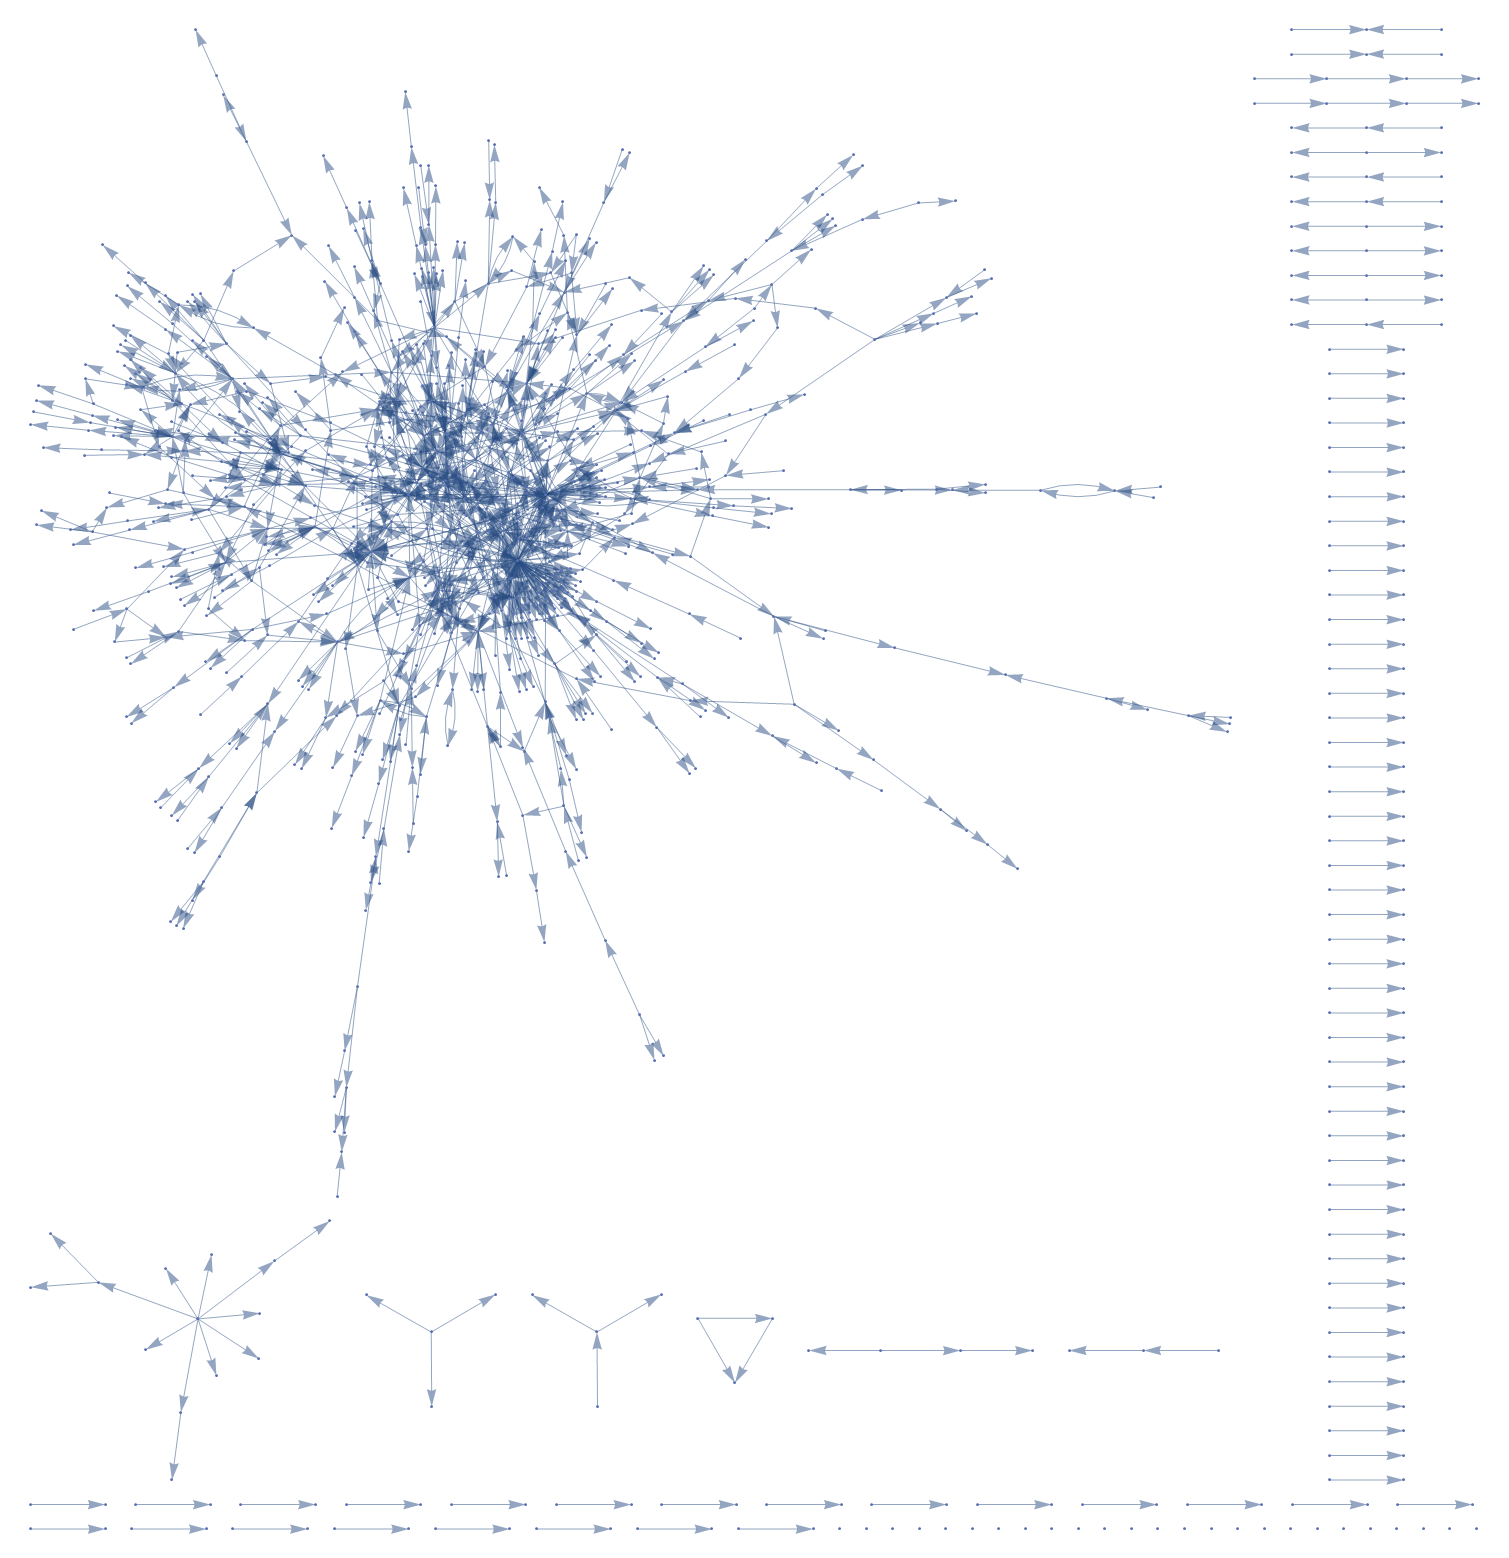
\includegraphics[width=\textwidth]{display_sciMet.png}
\caption{The SciMet network dataset used in our Table \ref{tab:network_table} comparison to $G$. Note the high number of connected components, and low number of children per parent, in contrast to the ``blooming" behavior in $G$ created by the inclusion of ALL child references from each parent paper.}
\label{fig:sciMet}
\end{figure}

\begin{figure}[H]
\centering
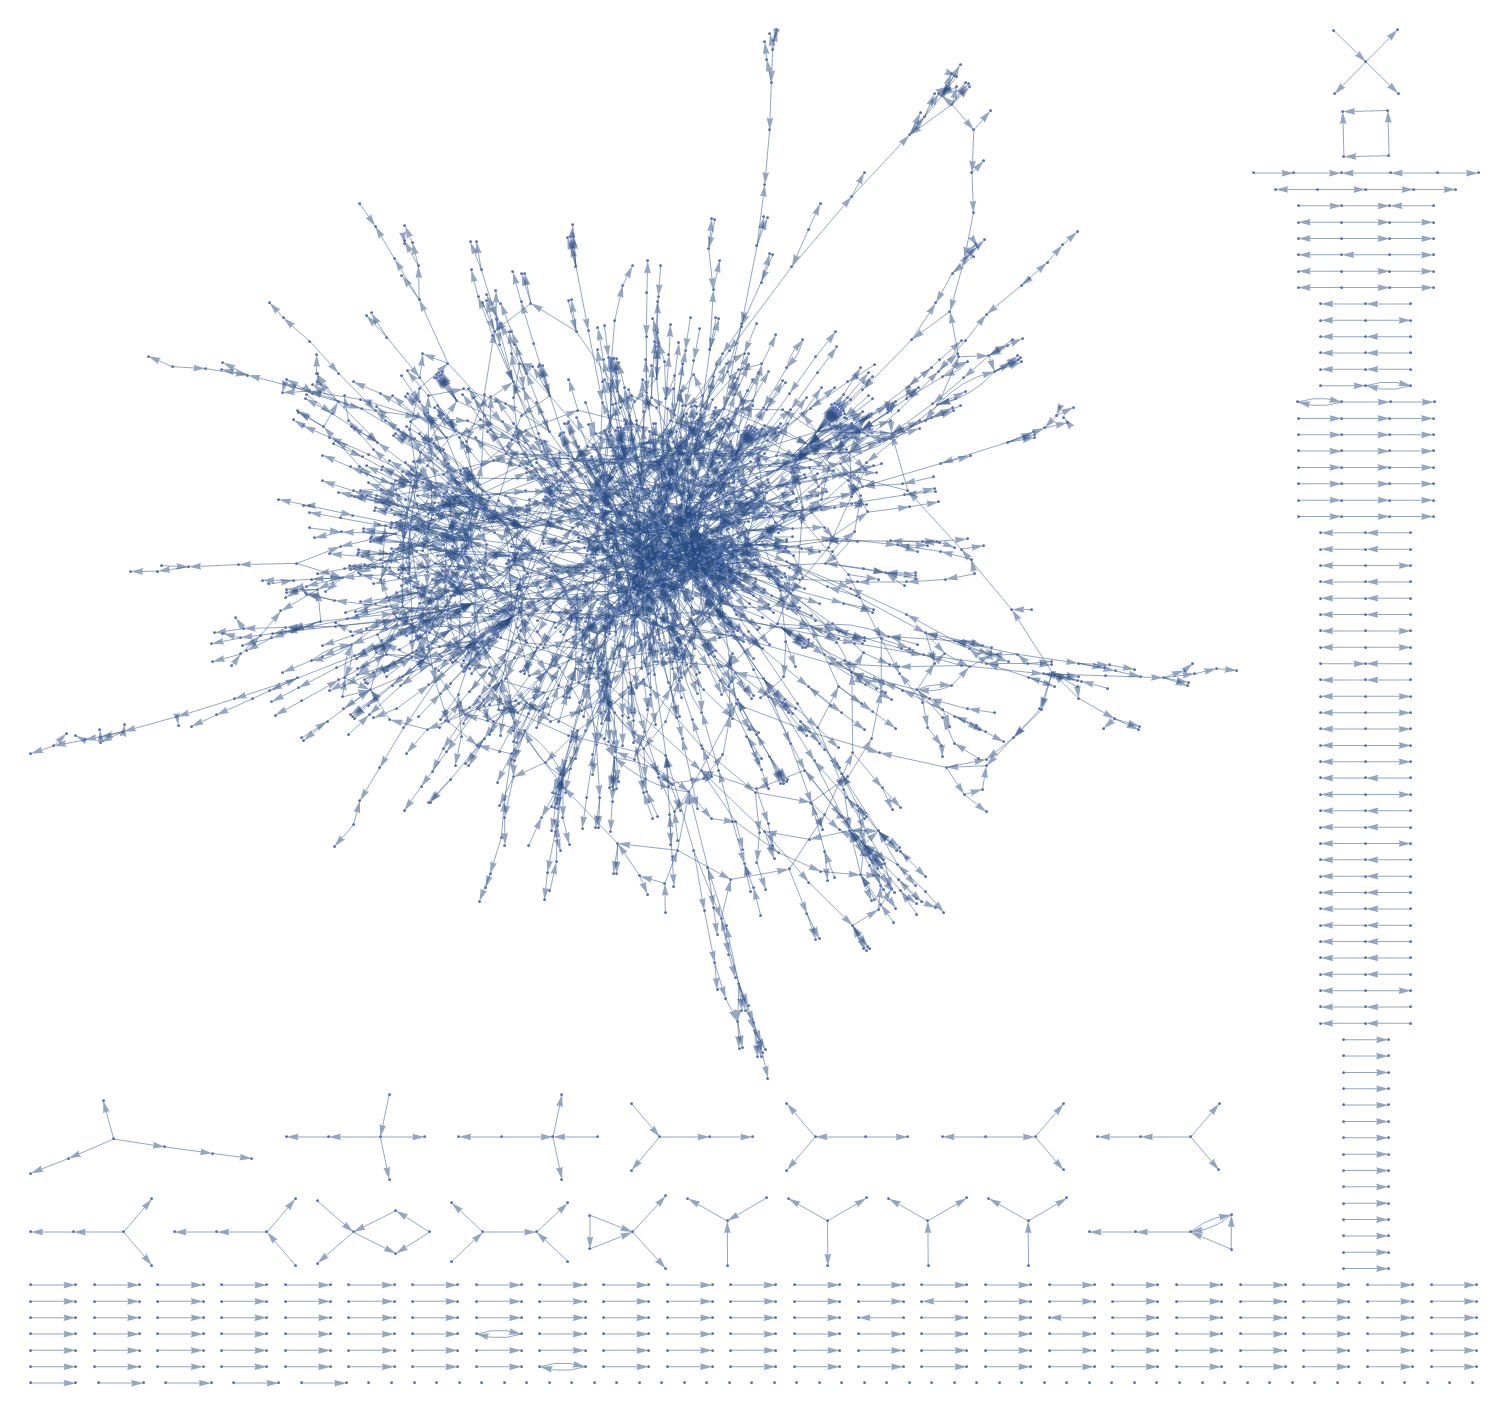
\includegraphics[width=\textwidth]{display_zewail.png}
\caption{The Zewail citation network dataset used in our Table \ref{tab:network_table} comparison to $G$. Note the high number of connected components, and low number of children per parent, in contrast to the ``blooming" behavior in $G$ created by the inclusion of ALL child references from each parent paper.}
\label{fig:zewail}
\end{figure}

\begin{figure}[H]
\centering
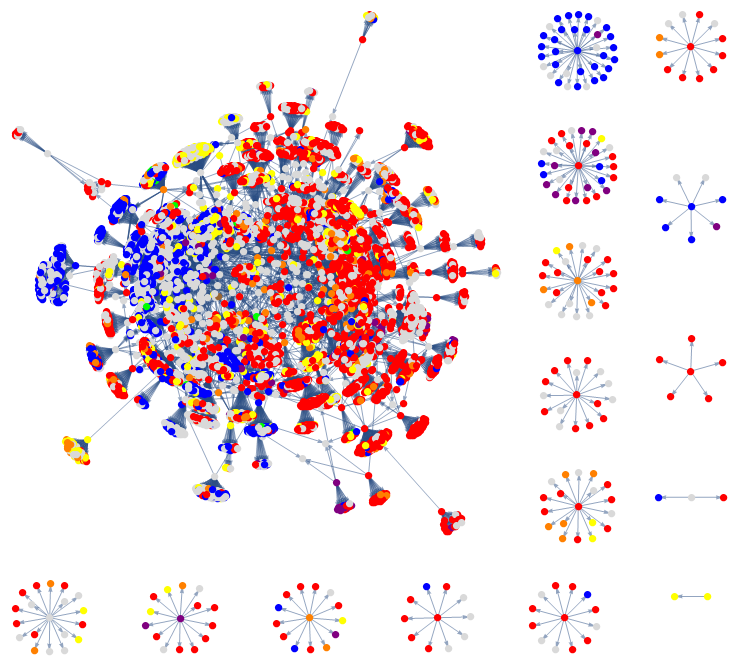
\includegraphics[width=\textwidth]{full_network_color_coded.png}
\caption{The full network $G_p$, with vertices colored according to their subject label as in Figure \ref{fig:subject_color_coded}.}
\label{fig:full_subject_color_coded}
\end{figure}

\begin{sidewaysfigure}
\centering
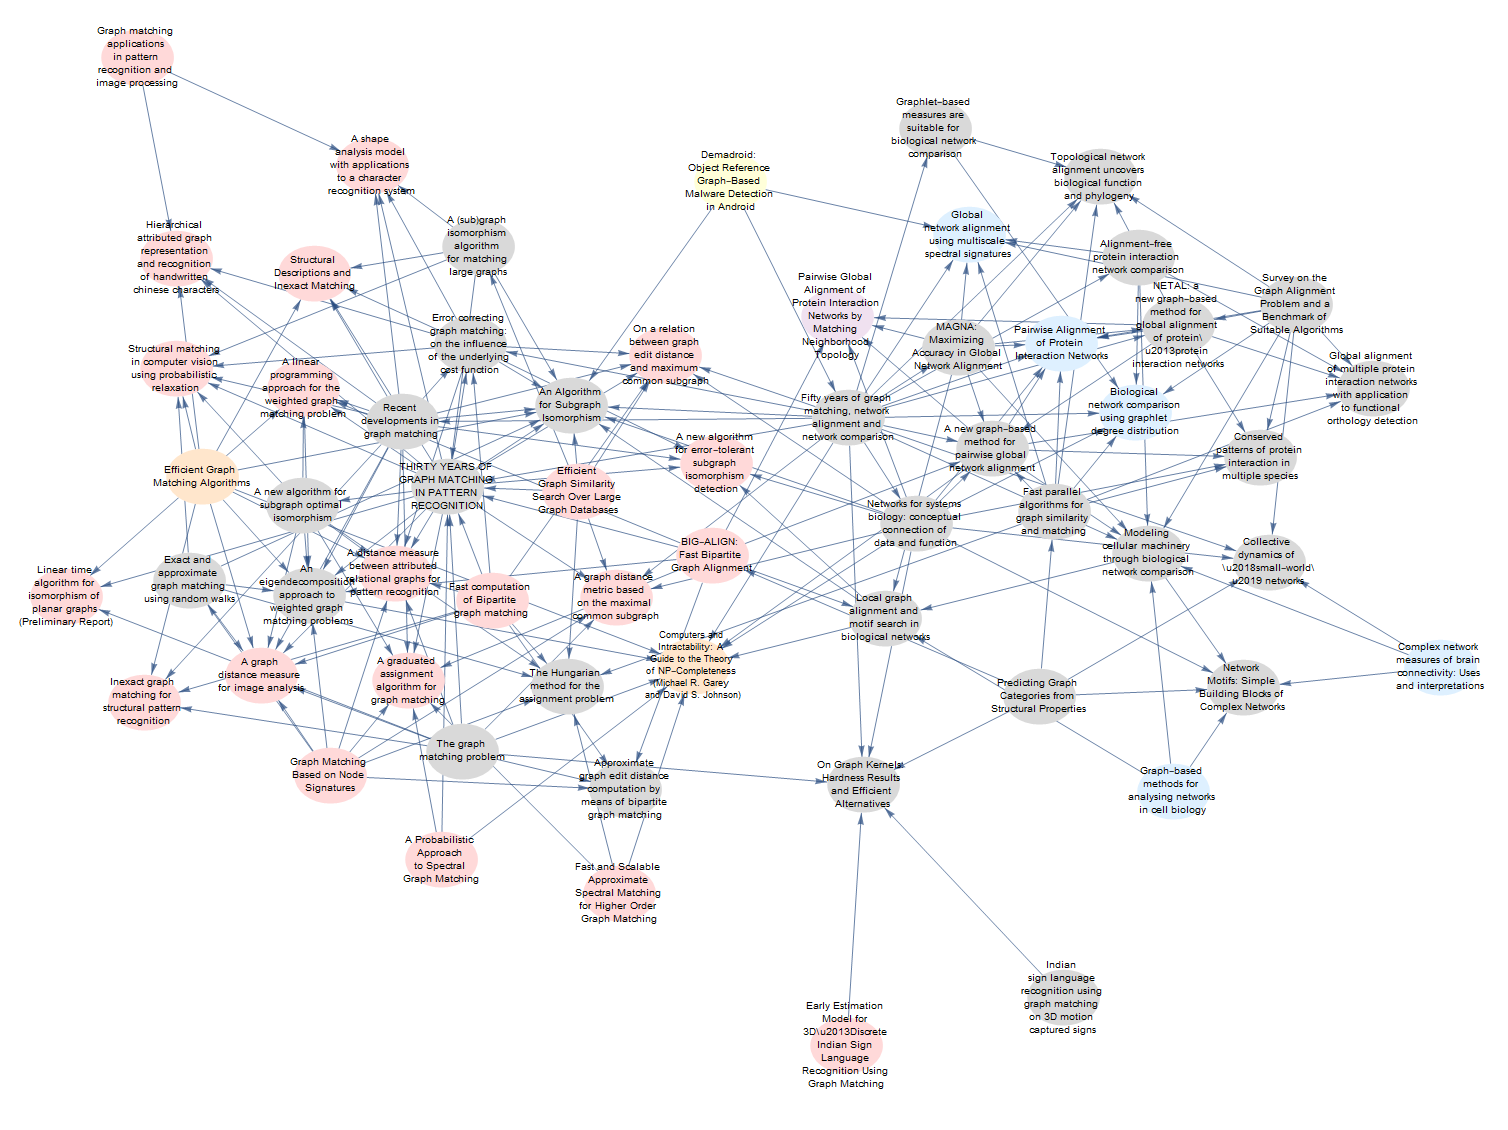
\includegraphics[width=0.85\textwidth]{reading_list_subject_colored_CROPPED.png}
\caption{The subnetwork $S$ of high centrality papers, as listed in Tables \ref{tab:toppapers_all}, \ref{tab:toppapers_bio}, and \ref{tab:toppapers_CS}, with vertices colored by subject label. Grey vertices are unlabeled, pink is computer science, blue is biology, yellow is math, orange is both math and computer science, and purple is both computer science and biology.}
\vspace{-12pt}\flushleft\scriptsize Note: ``Unsupervised Domain Adaptation Using Regularized Hyper-Graph Matching" is not in the connected component and is not displayed.
\label{fig:reading_list_subject_colored}
\end{sidewaysfigure}


\begin{table}[t]
\centering
\setlength\extrarowheight{3pt}
\begin{tabular}{|l|r|r|r|}
\hline & $G_R$ & $G_R^{(1)}$ & $G_R^{(2)}$ \\ \hline\hline
Total vertices & 61 & 27 & 34 \\ \hline
Untagged & 30 & 8 & 22 \\ \hline
Tagged & 31 & 19 & 12 \\ \hline
CS & 24 & 2 & 22 \\ \hline
Biology & 6 & 6 & 0 \\ \hline
Math & 3 & 1 & 2 \\ \hline
Both CS and biology & 1 & 1 & 0 \\ \hline
Both CS and math & 2 & 0 & 2 \\ \hline
Both biology and math & 0 & 0 & 0 \\ \hline
All three & 0 & 0 & 0 \\ \hline
\end{tabular}
\caption{Number of vertices tagged as computer science, biology, math, or some combination of these in the reading list subnetwork $G_R$, and its intersections $G_R^{(1)}$ and $G_R^{(2)}$ with the two halves of the partition $G_p^{(1)}$ and $G_p^{(2)}$. See Table \ref{tab:subject_counts}.}
\label{tab:reading_list_subject_counts}
\end{table}

%\begin{singlespace}
%\begin{longtable}{|L{0.095\textwidth}|C{0.04\textwidth}|C{0.045\textwidth}|C{0.045\textwidth}|L{0.7\textwidth}|}
%\hline
%Subject & $N$ & $G_R^{(1)}$ & $G_R^{(2)}$ & Title \\ \hline
%\hline
%\endhead
%None & 22 & 15 & 7 & Fifty years of graph matching, network alignment and network comparison \\ \hline
%None & 15 & 10 & 5 & Networks for systems biology: conceptual connection of data and function \\ \hline
%Biology & 7 & 7 & 0 & Global network alignment using multiscale spectral signatures \\ \hline
%None & 13 & 1 & 12 & Error correcting graph matching: on the influence of the underlying cost function \\ \hline
%None & 10 & 10 & 0 & MAGNA: Maximizing Accuracy in Global Network Alignment \\ \hline
%None & 4 & 4 & 0 & Graphlet-based measures are suitable for biological network comparison \\ \hline
%None & 7 & 6 & 1 & On Graph Kernels: Hardness Results and Efficient Alternatives \\ \hline
%Biology & 8 & 8 & 0 & Pairwise Alignment of Protein Interaction Networks \\ \hline
%None & 6 & 6 & 0 & Alignment-free protein interaction network comparison \\ \hline
%Biology & 7 & 7 & 0 & Biological network comparison using graphlet degree distribution \\ \hline
%None & 10 & 10 & 0 & NETAL: a new graph-based method for global alignment of protein-protein interaction networks \\ \hline
%CS/Math & 10 & 4 & 6 & Computers and Intractability: A Guide to the Theory of NP-Completeness \\ \hline
%None & 16 & 1 & 15 & Recent developments in graph matching \\ \hline
%None & 10 & 10 & 0 & Modeling cellular machinery through biological network comparison \\ \hline
%CS & 7 & 2 & 5 & A graph distance metric based on the maximal common subgraph \\ \hline
%None & 24 & 1 & 23 & Thirty years of graph matching in pattern recognition \\ \hline
%None & 6 & 6 & 0 & Collective dynamics of ``small-world" networks \\ \hline
%None & 13 & 11 & 2 & A new graph-based method for pairwise global network alignment \\ \hline
%None & 12 & 4 & 8 & An Algorithm for Subgraph Isomorphism \\ \hline
%CS & 8 & 2 & 6 & On a relation between graph edit distance and maximum common subgraph \\ \hline
%None & 7 & 7 & 0 & Topological network alignment uncovers biological function and phylogeny \\ \hline
%CS & 7 & 0 & 7 & A linear programming approach for the weighted graph matching problem \\ \hline
%None & 10 & 0 & 10 & An eigendecomposition approach to weighted graph matching problems \\ \hline
%CS & 8 & 0 & 8 & A graduated assignment algorithm for graph matching \\ \hline
%None & 9 & 0 & 9 & A new algorithm for subgraph optimal isomorphism \\ \hline
%CS & 9 & 0 & 9 & A distance measure between attributed relational graphs for pattern recognition \\ \hline
%CS & 5 & 0 & 5 & Inexact graph matching for structural pattern recognition \\ \hline
%CS & 6 & 2 & 4 & A new algorithm for error-tolerant subgraph isomorphism detection \\ \hline
%CS & 6 & 0 & 6 & Structural Descriptions and Inexact Matching \\ \hline
%CS & 6 & 0 & 6 & A shape analysis model with applications to a character recognition system \\ \hline
%CS & 9 & 0 & 9 & A graph distance measure for image analysis \\ \hline
%CS & 8 & 0 & 8 & Structural matching in computer vision using probabilistic relaxation \\ \hline
%CS & 6 & 0 & 6 & Hierarchical attributed graph representation and recognition of handwritten chinese characters \\ \hline
%CS & 4 & 0 & 4 & Linear time algorithm for isomorphism of planar graphs (Preliminary Report) \\ \hline
%CS/Bio & 6 & 5 & 1 & Pairwise Global Alignment of Protein Interaction Networks by Matching Neighborhood Topology \\ \hline
%None & 6 & 6 & 0 & Conserved patterns of protein interaction in multiple species \\ \hline
%None & 5 & 0 & 5 & Approximate graph edit distance computation by means of bipartite graph matching \\ \hline
%None & 8 & 4 & 4 & Local graph alignment and motif search in biological networks \\ \hline
%None & 6 & 6 & 0 & Network Motifs: Simple Building Blocks of Complex Networks \\ \hline
%None & 8 & 1 & 7 & The Hungarian method for the assignment problem \\ \hline
%CS & 9 & 0 & 9 & Graph Matching Based on Node Signatures \\ \hline
%None & 7 & 0 & 7 & Exact and approximate graph matching using random walks \\ \hline
%None & 6 & 6 & 0 & Global alignment of multiple protein interaction networks with application to functional orthology detection \\ \hline
%None & 10 & 9 & 1 & Fast parallel algorithms for graph similarity and matching \\ \hline
%CS & 9 & 0 & 9 & Fast computation of Bipartite graph matching \\ \hline
%CS & 4 & 0 & 4 & Fast and Scalable Approximate Spectral Matching for Higher Order Graph Matching \\ \hline
%CS & 4 & 0 & 4 & A Probabilistic Approach to Spectral Graph Matching \\ \hline
%CS & 3 & 0 & 3 & Graph matching applications in pattern recognition and image processing \\ \hline
%None & 10 & 1 & 9 & The graph matching problem \\ \hline
%Biology & 4 & 4 & 0 & Graph-based methods for analysing networks in cell biology \\ \hline
%CS & 10 & 4 & 6 & BIG-ALIGN: Fast Bipartite Graph Alignment \\ \hline
%None & 7 & 0 & 7 & A (sub)graph isomorphism algorithm for matching large graphs \\ \hline
%Biology & 4 & 4 & 0 & Complex network measures of brain connectivity: Uses and interpretations \\ \hline
%CS & 7 & 0 & 7 & Efficient Graph Similarity Search Over Large Graph Databases \\ \hline
%3 & 4 & 3 & 1 & Demadroid: Object Reference Graph-Based Malware Detection in Android \\ \hline
%None & 2 & 2 & 0 & Indian sign language recognition using graph matching on 3D motion captured signs \\ \hline
%None & 6 & 5 & 1 & Predicting Graph Categories from Structural Properties \\ \hline
%None & 10 & 10 & 0 & Survey on the Graph Alignment Problem and a Benchmark of Suitable Algorithms \\ \hline
%CS/Math & 12 & 0 & 12 & Efficient Graph Matching Algorithms \\ \hline
%CS & 2 & 2 & 0 & Early Estimation Model for 3D-Discrete Indian Sign Language Recognition Using Graph Matching \\ \hline
%None & 1 & 0 & 1 & Unsupervised Domain Adaptation Using Regularized Hyper-Graph Matching \\ \hline
%\caption{Number of vertices in the neighborhood of each paper in $G_R$, and how many vertices in it lie on each side of the partition.}
%\label{tab:neighborhood_partition_counts}
%\end{longtable}
%\end{singlespace}

\begin{table}[t]
\centering
\setlength\extrarowheight{1.5pt}
\begin{tabular}{| l | l |}
\hline
\textbf{Usage} & \textbf{Package Name(s)} \\ \hline\hline
Mathematical Computation & NumPy \\
& NetworkX \\
\hline
Figure creation* & Matplotlib \\ 
\hline
File I/O Handling & csv\\ 
& glob \\
& re \\
\hline
API Request Handling  & urllib \\
& Requests \\ 
& time \\
\hline
Interfacing with Google Sheets & gspread$^\Diamond$ \\
& oauth2client$^\Diamond$ \\
\hline
The \verb+defaultdict+ datatype & collections \\
\hline
Interfacing my own modules with Jupyter notebooks & importlib$^\Diamond$ \\ 
\hline
\end{tabular}
\caption{Python packages used for the project. All but those marked with a $\Diamond$ are found in either the standard library or available in Anaconda for Python 3.6 on 64-bit Windows in mid-2018, and the remainder can be installed via pip.}
\footnotesize *Only Figure \ref{fig:year_distributions} was created in Python. The remainder were made in Mathematica.
\label{tab:python_packages}
\end{table}

%\begin{figure}[p]
%\textbf{Initial loading of $G$, sciMet, and zewail GML files}
%\begin{verbatim}
%G = Import["citation_network.gml"]
%sciMet = Import["sciMet_dataset.gml"]
%zewail = Import["zewail_dataset.gml"]
%\end{verbatim}
%\textbf{Creating the pruned network $G_p$.}
%\begin{verbatim}
%parents = Position[VertexOutDegree[G], _?(# > 0 &)] // Flatten;
%popular = Position[VertexInDegree[G], _?(# > 1 &)] // Flatten;
%pruned = Subgraph[G, Union[parents, popular], Options[G]];
%Gp = Subgraph[pruned, WeaklyConnectedComponents[pruned][[1]], 
%    Options[pruned]]
%\end{verbatim}
%\textbf{Creating the random network $R$.}
%\begin{verbatim}
%R = RandomGraph[{VertexCount[G], EdgeCount[G]}, DirectedEdges -> True]
%\end{verbatim}
%\textbf{Creating the random network $R_d$ with the same degree sequences as $G$.}
%\begin{verbatim}
%outStubs = VertexOutDegree[G];
%inStubs = VertexInDegree[G];
%vertexlist = Range[VertexCount[G]];
%edgelist = {};
%For[i = 1, i <= EdgeCount[g], i++,
% source = RandomSample[outStubs -> vertexlist, 1][[1]];
% target = RandomSample[inStubs -> vertexlist, 1][[1]];
% outStubs[[source]] -= 1;
% inStubs[[target]] -= 1;
% AppendTo[edgelist, source -> target];]
%Rd = Graph[vertexlist, edgelist];
%\end{verbatim}
%\caption{The Mathematica code used to create the networks analyzed in Table \ref{tab:network_table}.}
%\label{fig:network_creation_source_code}
%\end{figure}

\begin{table}[p]
\centering
\begin{tabular}{| l | l | l |}
\hline
\textbf{Computer Science} & \textbf{Biology} & \textbf{Mathematics} \\ \hline\hline
ACM & Biochem- & Algebra \\
Algorithm & Biocomputing & Algorithm \\
Artificial Intelligence & Bioengineering & Chaos \\
CIVR & Bioinformatic & Combinatori- \\
Computational Intelligence & Biological & Fixed Point \\
Computational Linguistics & Biology & Fractal \\
Computer & Biomedic- & Functional Analysis \\
Computer Graphics & Biosystem & Geometr- \\
Computer Science & Biotechnology & Graph \\
Computer Vision & Brain & Kernel \\
Data & Cancer & Linear Regression \\
Data Mining & Cardiology & Markov \\
Document Analysis & Cell & Mathemati- \\
Electrical Engineering & Disease & Multivariate \\
Graphics & DNA & Network \\
IEEE & Drug & Optimization \\
Image Analysis & Endocrinology & Permutation Group \\
Image Processing & Epidemiology & Probability \\
Intelligent System & Genetic & Riemann Surface \\
Internet & Genome & SIAM \\
ITiCSE & Genomic & Statistic- \\
Language Processing & Medical & Topology \\ 
Learning & Medicinal & Wavelet \\
Machine Learning & Medicine & \\
Machine Vision & Metabolic & \\
Malware & Microbiology & \\
Neural Network & Molecular & \\
Pattern Recognition & Neuro- & \\ 
Robotic & Neurobiological & \\
Scientific Computing & Pathology & \\
SIAM & Pathogen & \\
Signal Processing & Pharma- & \\
Software & Plant & \\
World Wide Web & Protein & \\
 & Proteom- & \\
 & Psych- & \\
 & Psychology & \\
 & Virology & \\
 & Virus & \\
\hline
\end{tabular}
\caption{Keywords used to tag journal names as various subjects.}
\vspace{-6pt}\flushleft\footnotesize *Note: Both a term and its plural are considered a match, and hyphens indicate a word with several ending variations which were all considered to be associated with the tag. While the search process was case sensitive in order to avoid false positives for short words like ``ACM", case-insensitive duplicate words have been excluded from the table. The words ``algorithm" and ``SIAM" are considered to be both computer science and mathematics.
\label{tab:tagging_keywords}
\end{table}


\bibliographystyle{plain}
\bibliography{thesis_bibliography}

% If you want to include an index, this prints the index at this location. You must have \makeindex uncommented in the preamble
\printindex

\end{document}